\chapter{Poincare map}
\newcommand{\dpmap}{\mathcal{D}\mathcal{P}}
\newcommand{\pmap}{\mathcal{P}}
\newcommand{\nfp}{n_\text{fp}}
\newcommand{\shear}{\alpha_s}
\newcommand{\qaxis}{q_a}
\newcommand{\z}{x}

In the study of continuous dynamical systems, it is often convenient to consider a discrete map defined by the intersection of the trajectories with a lower-dimensional subspace and which captures some properties of the continuous case. For particles following the magnetic field of a toroidal apparatus, the intersection of their trajectories with a constant $\phi$ cross-section reveals the distinct region of different field line behaviour~: closed surfaces, islands, chaotic regions, and is known as a \textit{Poincare} section.

\begin{figure}[H]
    \centering
    \begin{subfigure}[c]{0.32\textwidth}
        \centering
        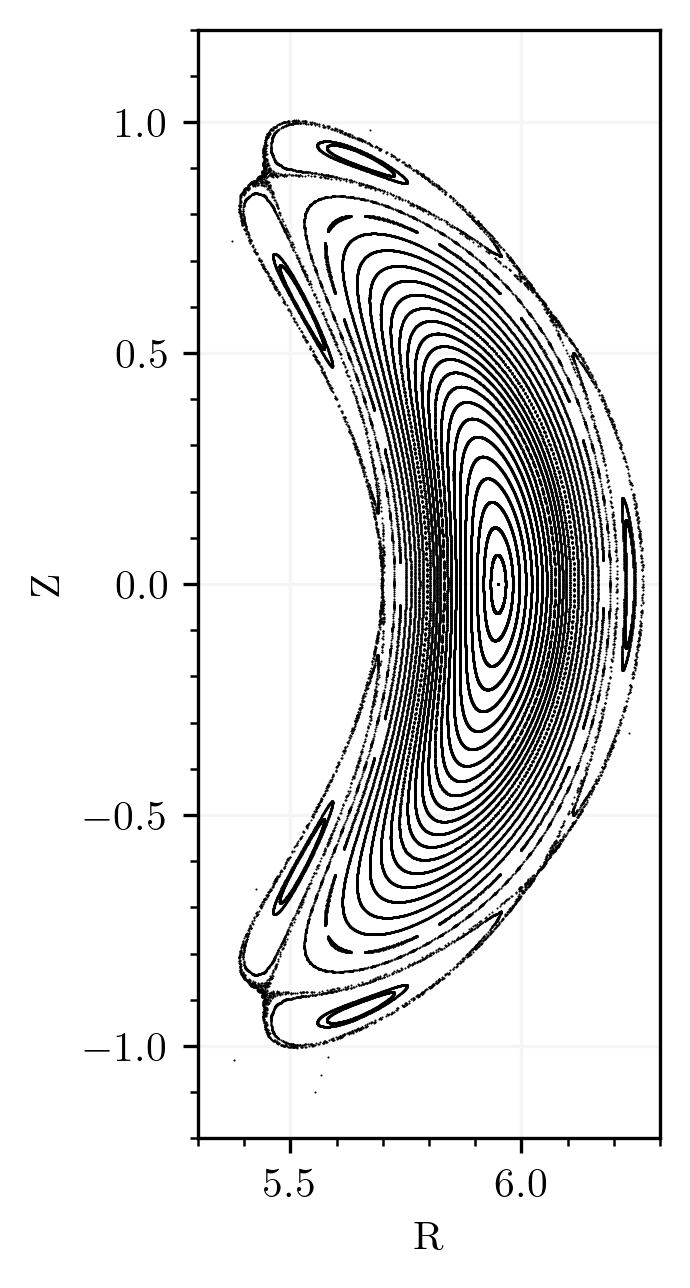
\includegraphics[width=\textwidth]{images/theory/w7x.png}
        \caption{W7-X, $\nfp = 5$}
        \label{fig:w7x-default}
    \end{subfigure}
    \hfill
    \begin{subfigure}[c]{0.32\textwidth}
        \centering
        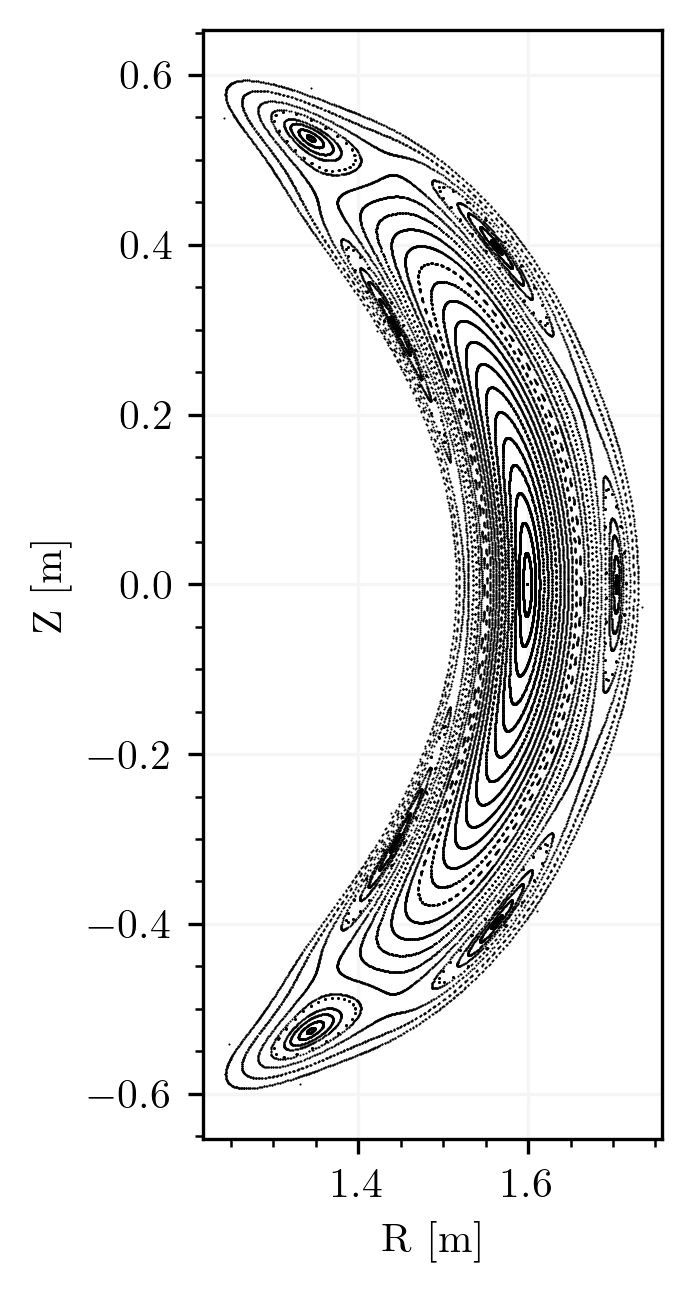
\includegraphics[width=\textwidth]{images/theory/ncsx.png}
        \caption{NCSX, $\nfp = 3$}
        \label{fig:ncsx-default}
    \end{subfigure}
    \hfill
    \begin{subfigure}[c]{0.32\textwidth}
        \centering
        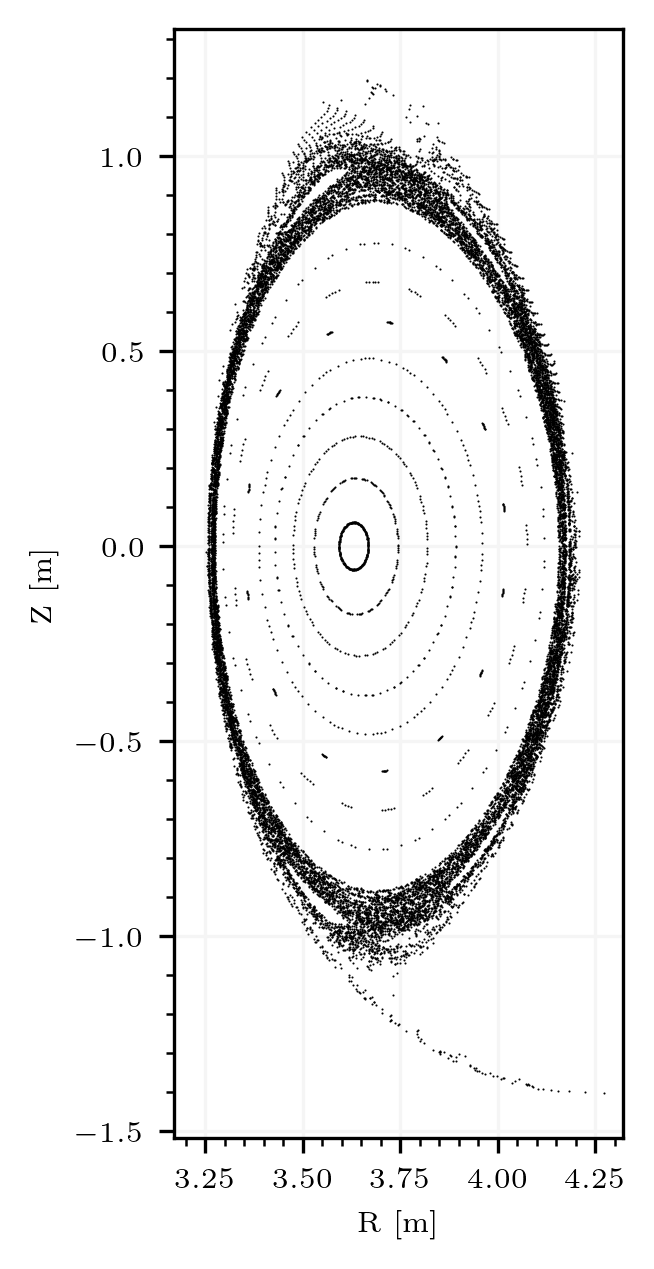
\includegraphics[width=0.94\textwidth]{images/theory/lhd.png}
        \caption{LHD, $\nfp = 10$}
        \label{fig:lhd-default}
    \end{subfigure}
    \caption{Poincare section at $\phi = 0$ for (a) Wendelstein-7X, (b) the (aborted) National Compact Stellarator Experiment and (c) the Large Helical Device stellarator. The field lines are trace using Runge Kutta Dopri5.}
    \label{fig:poincare-example}
\end{figure}

Using Biot-Savart law to get the field generated from the known currents and coil geometry and by neglecting the gyro-motion around the field lines, the crossings can be numerically recorded. In \figref{fig:poincare-example} the Poincaré sections for three well known devices are computed using Runge-Kutta integration scheme. The closed flux surfaces appear from the magnetic axis up to the edge region. For W7-X and NCSX configuration, one island is predominant. For LHD on the contrary, the edge region is chaotic and multiple small islands are present in the chaotic edge region. Such a figure can be produced experimentally in stellarators by firing an electron beam, sweeping a fluorescent rod and using a long camera exposure \cite{pedersen_confirmation_2016}. To define a map that gives the evolution of the position of the crossings in the $\phi$ semi-plane, first note that for each initial point $\textbf{x}_0$ there is an associated curve $\gamma(t)$ depending on time which is link to the flow $\gamma(t) = \Phi(\textbf{x}_0, t)$ of the magnetic vector field. The cylindrical coordinates are a natural choice here.

\noindent
\makebox[\textwidth]{%
  \begin{tcolorbox}[colback=lightgray!10, colframe=black, width=0.85\textwidth, boxrule=0.5mm, sharp corners]
    \textbf{Geometric consideration} : Throughout this document, the convention adpoted is that of the contravariant component for vectors. That is, for example, $\textbf{B}$ in cylindrical coordinates has the form $B^R = \textbf{B}\cdot\nabla R$, $B^\phi = \textbf{B}\cdot\nabla\phi$ and $B^Z = \textbf{B}\cdot\nabla Z$. In the formalism of differential geometry, one writes $B=B^i\partial_i$. The basis $\{\partial_i\}_i$ is orthogonal and holonomic but the element may not be unitary, as for $\partial_\phi$. On the other hand, the component in the common orthonormal basis $e_i$ will be written with subscript as $\tilde{B}^i$. [SEE APP]
  \end{tcolorbox}
}

The trajectory curve $\gamma : \mathbb{R}^+ \rightarrow \mathbb{R}^+\times[0,2\pi[\times\mathbb{R} \eqqcolon \mathcal{M}$, $t \mapsto \gamma(t) = (R(t),\,\phi(t),\,Z(t))$ we are interested in is such that the tangent vector at each point is given by $\dot{\gamma}(t)= \textbf{B} = B^i\partial_i \in T_{\gamma(t)}\mathcal{M}$. Specifying the initial point $\gamma(0) = \textbf{x}_0$ identifies a specific curve~:
\begin{align*}
    \gamma(t) = \int_0^t\dot{\gamma}(s)ds + \textbf{x}_0 \quad \text{with} \quad   \dot{\gamma}^i(t)= (\frac{dR}{dt},\,\frac{d\phi}{dt},\,\frac{dZ}{dt}) = (B^R, B^\phi, B^Z).
\end{align*}
Provided that the sign of $B^\phi(R, \phi, Z)$ is either positive or negative on $\gamma$, $B^\phi$ is never zero, the map~:
\begin{equation*}
    t(\phi) = \int \frac{dt}{d\phi}d\phi = \int_0^\phi \frac{1}{B^\phi}d\phi
\end{equation*}

defines a handy change of variable for which the $\phi$ evolution is linear. Indeed $\gamma$ can be re-parameterized as $\phi \mapsto \gamma(\phi) = (R(\phi),\,\phi,\,Z(\phi))$ with~$\dot{\gamma}$~:
\begin{equation*}
    \dot{\gamma}^i(\phi) = (\frac{dR}{d\phi},\,1,\,\frac{dZ}{d\phi}) = (\frac{dR}{dt}\frac{dt}{d\phi},\,1,\,\frac{dZ}{dt}\frac{dt}{d\phi}) = (B^R/B^\phi,\, 1,\,B^Z/B^\phi).
\end{equation*}
Due to the choice of coordinates the field will have at most a $\phi$ periodicity of $2\pi$, yet in stellarator configurations have azymuthal redundancy. Their period is $T = 2\pi/n_\text{fp}$ where $n_\text{fp}\in\mathbb{N}^\star$ is the number of field period in a complete toroidal rotation. For example, W7X and LHD have 5 and 10 field periods respectively. If the field is not periodic then $n_\text{fp} = 1$ and, in contrast, for an axisymmetric device $n_\text{fp} = +\infty$, the case of ideal Tokamaks.

The Poincare section is identical for $\phi_i$ and $\phi_i+kT$, $k\in\mathbb{Z}$. Writing $\Omega$ the set of initial points in the $\phi_i$ plane for which $\gamma$ is effectively re-parametrizable between $\phi_i$ and $\phi_i + T$, allows to define the map $\pmap : \Omega \rightarrow \mathbb{R}_+\times\mathbb{R}$ as~:
\begin{equation}\label{eq:pmap}
    (\tilde{R},\tilde{Z}) \mapsto \pmap(\tilde{R},\tilde{Z}) = \int_{\phi_i}^{\phi_i+T}(
        \dot{\gamma}^R(s),\,
        \dot{\gamma}^Z(s)
    )\,ds + (\tilde{R},\tilde{Z})
\end{equation}
with $\textbf{x}_0 = (\tilde{R},\,\phi_i,\,\tilde{Z})$. 
The point $(R,Z) \in \Omega$ are point in the initial section and should not be confused with the $\gamma^R$ and $\gamma^Z$ components.


\figref{fig:th-poincare-map} represent an hypothetical $\nfp = 3$ configuration where an initial starting point $z_0\coloneqq (\tilde{R}_i,\tilde{Z}_i)$ gets map to the $\phi_i + T$ cross section. The evolution of the intersection for $z_0$ is then simply $z_{i+1} = \pmap(z_i)$ and $z_n = \pmap^n(z_0)$. 

\begin{figure}[H]
    \centering
    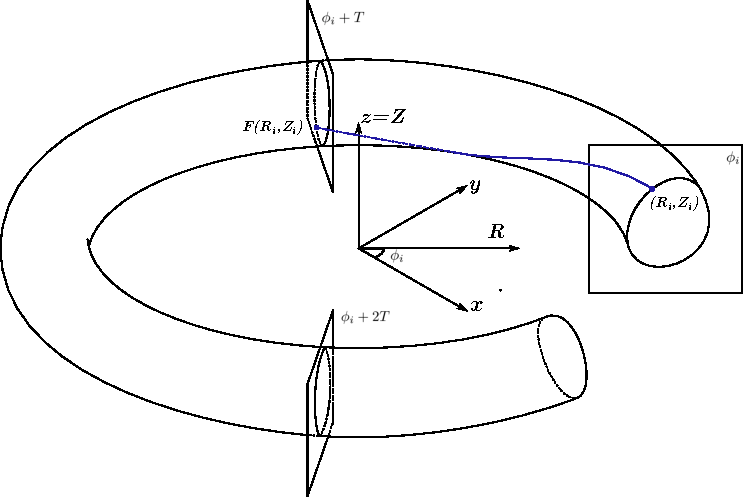
\includegraphics{images/theory/poincare-torus.pdf}
    \caption{Trajectory of a particle in a toroidal device (Tokamak/Stellarator) from a starting point $(\tilde{R}, \tilde{Z})$ in a $\phi = \phi_i$ section to a point in the $\phi = \phi_i + T$ plane with $T$ the azymuthal periodicity of the magnetic field.}
    \label{fig:th-poincare-map}
\end{figure}

As the evolution is performed by following $\mathbf{B}$ and due to the magnetic field been divergence free $\nabla\cdot\textbf{B} = 0$, the flux through any surface obtained by mapping a simple path in $\phi_i$ to $\phi_i + T$ will be zero. This result in the key property of $\pmap$ being flux-conserving ; the flux through any closed surface $\Sigma \subset \Omega$ is equal to the one through $\pmap(\Sigma)$~:
\begin{equation*}
    \iint\limits_{\Sigma}\textbf{B}\cdot\textbf{dS} = \iint\limits_{\pmap(\Sigma)}\textbf{B}\cdot\textbf{dS}.
\end{equation*}
The determinant of the Jacobian matrix for a general flow $\Phi(\textbf{x}_0, t)$ of a vector field $v$, which does not depend on time, is related to the divergence of $v$ \cite[p.408]{hirsch_differential_2013} by~:
\begin{equation}\label{eq:det-div-flow}
    \text{det}(\mathcal{D}\Phi(\textbf{x}_0, t)) = \text{det}(\mathcal{D}\Phi(\textbf{x}_0, 0))\exp\left(\int_0^t\text{Tr}(\nabla v(s)) ds\right) = \exp\left(\int_0^t \nabla\cdot v(s) ds\right)
\end{equation}
with $v(\Phi(\textbf{x}_0, s))$ written implicitly as $v(s)$. In the case of the flow in cylindrical coordinates, \citeauthor{wei_invariant_2023} use \equref{eq:det-div-flow} to derive the relation~(Eq.8):
\begin{equation*}\label{eq:det-div-pmap}
    \text{det}(\mathcal{D}\Phi(\textbf{x}_0, \phi_i, \phi_e)) = \exp\left(\int_{\phi_i}^{\phi_e} \frac{R\,(\nabla\cdot v)}{\tilde{v}^\phi} ds\right)\frac{\tilde{v}^\phi(\phi_i)}{\tilde{v}^\phi(\phi_e)}.
\end{equation*}
It gives for the determinant of $\dpmap \in \mathbb{R}^{2\times2}$ that~:
\begin{equation}\label{eq:pmap-det}
    \text{det}(\dpmap(\tilde{R}, \tilde{Z})) = B^\phi(\tilde{R},\phi_i, \tilde{Z})/B^\phi(\pmap^{\tilde{R}}(\tilde{R},\tilde{Z}), \phi_i+T,\pmap^{\tilde{Z}}(\tilde{R},\tilde{Z})).
\end{equation}
The last identity may also be recovered more directly using differential forms as in \cite{meiss_thirty_2015}, the derivation is given in \appref{forms}.

\section{Fixed points}

The map $\nmap$ \equref{eq:pmap} defines a map from $\Omega$ to $\Omega$. Such a map has interesting properties. Take for example Brouwers' fixed point theorem, e.g. \cite{michel_chipot_handbook_2008}, which states that any map from the disk to the disk has at least one fixed point. This means that there must be at least one point, which through the field line map, ends up exactly where it started! In fusion this point, and the field line through it has a special name, it is called the `magnetic axis' (and is often used as the `axis' of a coordinate system constructed on the basis of a magnetic field). More generally, a point $\x^\star\in\Omega$ that is mapped to itself after $k$ iteration of the field line map is part of a periodic orbits, representing the crossing of a closed field line.

The magnetic field twist around the magnetic axis in order to average out the $\nabla\textbf{B}$ drift. The twisting is quantify by the rotational transform $\iotaslash$ which indicates the fraction of poloidal turns performed after one toroidal turn. When $\iotaslash = n/m$ is rational, each field line rotates an angle $2\pi\iotaslash$. That means that each field line comes back to where it started after at most $m$ complete transits around the torus. For such a surface, it can be energetically more favorable to break up into an 'island chain'; instead of every field line returning to the same surface, there remains one closed field line around which the other field lines wind around, called the o-point of the island, and another field line with winding number m/n of that surface called the x-point. 

In Tokamaks, islands break the axisymmetry of the field and reduce confinement and they are unwanted. The action by which they are created is called a 'tearing mode', as the unbroken surfaces are 'torn open'. In Stellarators, there is no underlying symmetry and the islands can be a present, static feature of the equilibrium. Sometimes, like in W7X they are even desired and optimized for, as they generate a divertor-like structure [CITE]. Due to its relation with magneto-hydrodynamic stability limit, it is also more common to use the safety factor $q=1/\iotaslash$.

X/O-points of a $\iotaslash = n/m$ magnetic island close after $m$ toroidal turns. As there is $\nfp$ symmetry planes in one turn, there are a fixed point of $\pmap^{m\cdot\nfp}$. But the minimum number of iterations to close the orbit $k\in\mathbb{N}^\star$ is called the order of the orbit and is not in general equal to $m\cdot\nfp$. After $k$ application of the field line map the winding around the axis is $\Delta\theta(k) = 2\pi\iotaslash\,k/\nfp = 2\pi\cdot n/m \cdot k/\nfp$. To make one full rotation $k$ must be $k = m\,\nfp/n$, which is the correct order for of the orbit. The number of island is the greatest common divider between $m$ and $n$.

The NCSX stellarator is with 3 field periods and an island in the edge with $\iotaslash = 3/7$, shown in \figref{fig:ncsx-default}. There is only $1 = \gcd(3,7)$ island that rotates around the axis and the number of application of $\pmap$ for one of its fixed point to loop around is $k = 7\cdot3/3 = 7$.

To distinguish between O and X points, the behaviour of nearby field lines can be described using the Taylor expansion~:
\begin{equation*}
    \pmap^k(\z^\star+\delta \z) = \z^\star + \langle\dpmap^k\vert_{\z^\star},\, \delta\z\rangle + \smallO(\Vert\delta\z\Vert^2).
\end{equation*}
Especially by looking at the eigenvalues $\lambda_1$ and $\lambda_2$ of the jacobian $\dpmap^k\vert_{\z^\star}$. Using \equref{eq:pmap-det}, the determinant of $\dpmap^k\vert_{\z^\star}$  is equal to 1 or equivalently it is an element of $\text{SL}(2,\mathbb{R})$. Depending on the value of the trace the eigenvalues are either~:
\begin{enumerate}
    \item Complex conjugate and of modulus 1 ; $\lambda_{1,2} = e^{\pm i\theta}$, when $\vert \text{Tr}(\dpmap^k\vert_{\z^\star})\vert < 2$. They indicate rotation around the fixed point. The nearby field lines rotates around this fixed point making it an O-point.
    \item Both real with $\vert\lambda_s\vert < 1$ and $\vert\lambda_u\vert > 1$, when $\vert \text{Tr}(\dpmap^k\vert_{\z^\star})\vert > 2$ and $\mathcal{R}$.
    \item $\lambda_1 = \lambda_2 = \pm 1$
\end{enumerate}

To find the fixed point of the field line map the Newton method will be used. The O-points are relatively simple to find when using an initial guess in the right region. For many X-points, the strong exponential behaviour around them make the jacobian matrix ill conditioned. The region of convergence is then very small. This might be show stopper for some higher order island where the initial starting guess need to be made in a too precise region. Around the xpoint of ncsx and of the toybox presented in next section.

\begin{figure}
    \centering
    \begin{subfigure}[t]{0.49\textwidth}
        \centering
        \includegraphics[width=\textwidth]{}
        \caption{\label{fig:fp-ncsx}}
    \end{subfigure}
    \hfill
    \begin{subfigure}[t]{0.49\textwidth}
        \centering
        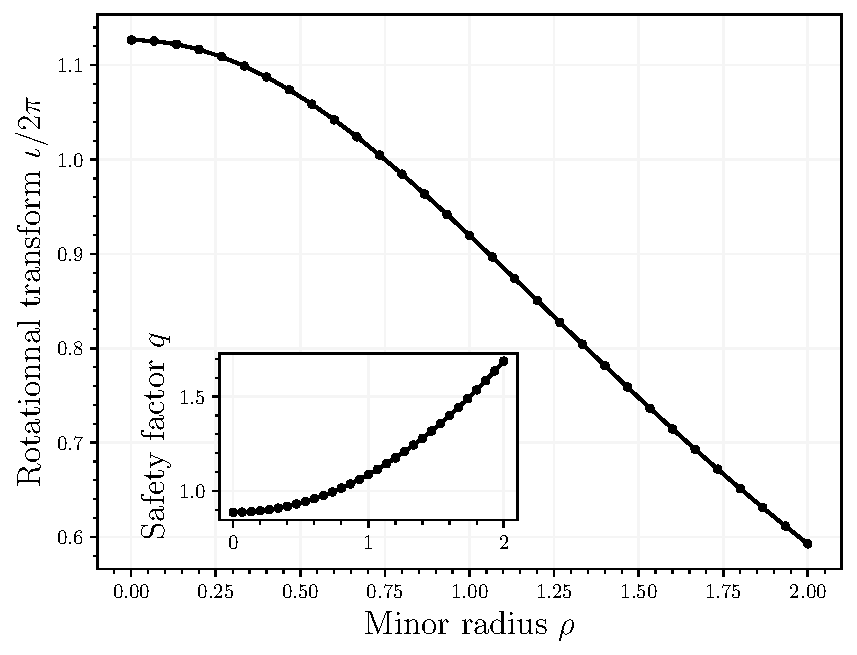
\includegraphics[width=\textwidth]{images/high-aspect-ratio/iota_q.pdf}
        \caption{\label{fig:fp-toybox}}
    \end{subfigure}
    \caption{}
    \label{fig:fp-search}
\end{figure}


%%% -- CHAPTER --- %%%
\chapter{Toybox}\label{ch:toybox}

An analytical magnetic geometry is introduced to provide a simpler and more flexible approach to the field line tracing analysis. This \textit{Toybox} is designed in cylindrical coordinates. Its baseline is the field of a high aspect ratio Tokamak equilibrium with quadratic q-profile, that can be tuned. On top of which the field generated by a circular current loop and perturbation can be added/removed and modified. It will be simpler than treating the geometry of a complex toroidal device and be handy to validate the numerical calculation of further algorithms. From the linearity of the curl operator, a sum of vector potentials $\textbf{A}_i$ has a one-to-one correspondence with the element of the resulting magnetic fields $\textbf{B}_i$. Defining the model in this way has the advantage of making it possible to use automatic differentiation from the 
\href{https://jax.readthedocs.io/en/latest/index.html}{\textcolor{blue}{\textit{JAX}}}
package \cite{bradbury_jax_2018}. The vector potential is the only quantity that needs to be defined analytically. The resulting $\textbf{B}$ or, in fact, any derivative of any reasonable order of $A$ can then be computed. The creation of a tokamak-like single null equilibrium is then the main focus.

More specifically in axisymmetric equilibria (i.e. perfect Tokamaks), following e.g \cite[p.108]{wesson_tokamaks_2011}, the shape of the magnetic surfaces are well defined by the flux function  $\psi$. Indeed, for cylindrical coordinates, all components/functions are constant along $\phi$, which yields~:
\begin{align*}
    \textbf{B} = B^i\partial_i = -\frac{1}{R}\frac{\partial\psi}{\partial Z}\partial_R +\frac{1}{R}\frac{\partial\psi}{\partial R}\partial_Z + \left(\frac{\partial A^R}{\partial Z} - \frac{\partial A^Z}{\partial R}\right)\partial_\phi.
\end{align*}
with $\psi = R^2 A^\phi$. The choice of Gauge can be exploited to assume $A^Z = 0$. For completeness, note that in the formulation of the Grad-Sharfranov equation, the last term, giving the $\phi$ component of the field, is related to a function $F(\psi)$ as $(\mu_0) F/R^2$.

A convenient geometry to study for the flux surfaces is nested toroids centered on the magnetic axis of RZ-coordinates $(R_0, Z_0)$. Introducing toroidal coordinates $(\rho, \phi, \theta)$, with $\rho$ the distance from the axis, the poloidal flux is thus $\psi(R, Z) \propto (R - R_0)^2 + (Z - Z_0)^2 = \rho^2$. In fact, due to the freedom in the dimension of the implementation, the equality can be choosen. For large aspect ratio tokamaks $R_0/\rho >> 1$ the safety factor profile can be approximated by~:
\begin{align*}
    q \approx \frac{\Delta\phi}{\Delta\theta} = \frac{\rho \tilde{B}^\phi}{R_0 \tilde{B}^\theta} = \frac{2\pi}{\mu_0\tilde{I}^\phi R_0} \rho^2
\end{align*}
calculating the multipole expansion of $\tilde{B}^\theta$ only up to first order. The $\tilde{B}^\phi$ component and the plasma current $\tilde{I}^\phi$ are imposed by the toroidal field coils and the central solenoid respectively. It would be desirable to achieve this quadratic behaviour of $q$ in the tokamak model as well. In more details, the $q$-profile can be calculated in a single $\phi$ section by integrating over the poloidal closed curve defined by $\psi = \text{const}$ \cite[pp.111-112]{wesson_tokamaks_2011}. In this specific case, as $\psi = \rho^2$, this path simply reduce to an integration over $\theta$ as~:
\begin{align}\label{eq:q-profile-th}
    q(\rho) = \frac{1}{2\pi}\int\limits_0^{2\pi} \frac{d\phi}{d\theta}d\theta = \frac{1}{2\pi}\int\limits_0^{2\pi} \frac{B^\phi}{B^\theta}d\theta.
\end{align}
The $\theta$ component can be derived directly from coordinate transformation, as follows~:
\begin{align*}
    B^\theta = \frac{\cos{\theta}}{\rho}B^Z - \frac{\sin{\theta}}{\rho}B^R = \frac{2}{R} = \frac{2}{R_0+\rho\cos{\theta}}.
\end{align*}
The $\phi$ component of $\textbf{B}$\footnote{In the implementation used in this document, the $B^\phi$ has been oriented along the -$\partial_\phi$ direction, which has no direct effect on the calculation themselves, but may occasionally cause some sign reversal, e.g. the latter value of the current in the circular loop coil. It also flips the way the field line rotate around the axis.} is introduced heuristically as~:
\begin{align*}
    B^\phi = 2\sqrt{R^2-\rho^2}\,(\qaxis+\frac{\shear}{2}\rho^2)/R^2
\end{align*}
with its corresponding $A^R$ provided in \appref{sec:jaxpot}. Inserting $B^\theta$ and $B^\phi$ in \eqref{eq:q-profile-th} gives~:
\begin{align*}
     q(\rho) = (\qaxis+\frac{\shear}{2}\rho^2)\frac{\sqrt{R^2-\rho^2}}{2\pi}\int\limits_{0}^{2\pi}\frac{1}{R_0 + \rho\cos{\theta}}d\theta = \qaxis+\frac{\shear}{2}\rho^2
\end{align*}
where the last two term cancel for $\rho < R$. At this point, we can make sense of the sf and shear constants as the on axis safety factor and the actual shear $dq/d\rho$. \figref{fig:toyha-basis-p} shows the cross section obtained by tracing the field line over a full toroidal revolution for the equilibrium with $R_0 = 6$, $Z_0 = 0$, $\qaxis = 0.8875$ and $\shear = 0.4$. While the effective number of field periods is $\nfp = \infty$, calculating the Poincare section by integrating over $2\pi$ remains correct even when perturbations are added and the axisymmetry breaks. The density of intersections is higher on the inside than on the outside. Since $B^\rho = 0$ and $\Tilde{B}^\phi/\tilde{B}^\theta \propto \sqrt{(\rho/R)^2-1}$ for constant $\rho$, a field line revolves faster in $\phi$ when $\theta \sim \pi$ then when $\theta \sim 0$ and thus make more crossings.

\begin{figure}
    \centering
    \begin{subfigure}[t]{0.43\textwidth}
        \centering
        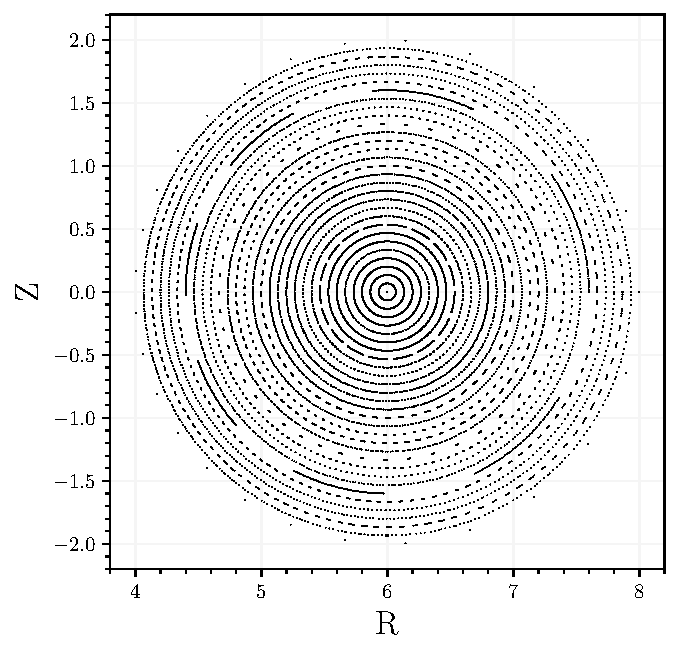
\includegraphics[width=\textwidth]{images/high-aspect-ratio/unperturbed.pdf}
        \caption{\label{fig:toyha-basis-p}}
    \end{subfigure}
    \hfill
    \begin{subfigure}[t]{0.54\textwidth}
        \centering
        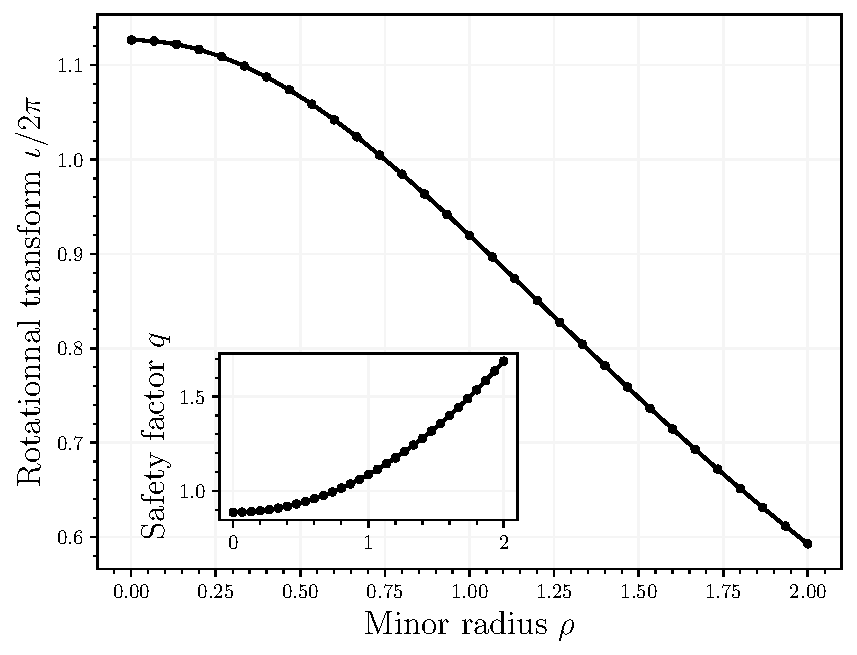
\includegraphics[width=\textwidth]{images/high-aspect-ratio/iota_q.pdf}
        \caption{\label{fig:toyha-basis-iotaq}}
    \end{subfigure}
    \caption{High aspect ratio Toy-Tokamak equilibrium with $R_0 = 6$, $Z_0 = 0$, $\qaxis = 0.8875$ and $\shear = 0.4$. (a) Poincar\'e section computed with Runge-Kutta algorithm. (b) Rotational transform $\iota/2\pi$ and $q$ profile with respect to the distance $\rho$ from the axis.}
    \label{fig:toyha-basis}
\end{figure}

The rotational transform $\iotaslash$ of field lines are computed by integrating both the field line themselves and the magnetic axis, tracking the evolution of the winding. Performing such a calculation for starting points of the form $(R_0+\rho,0)$ with $\rho\in [0, 2]$ gives the $\iotaslash$ profile in \figref{fig:toyha-basis-iotaq}. The calculated $q$-profile is in great agreement with its analytical form, which is reassuring.

An essential feature of the diverted tokamak edge structure is the separatrix. Combining a quadratic $q$ equilibrium with the field generated by a circular current loop at appropriate position and amplitude will result in a single null equilibrium. The vector potential of a curent loop at position $(R_l, 0)$ is given in \cite{simpson_simple_2001} as~:
\begin{align*}
    A^\phi = \frac{\mu_0}{4\pi}\frac{4IR_l}{\beta R}\left(\frac{(2-k^2)K(k^2)-2E(k^2)}{k^2}\right).
\end{align*}
with $K, E$ the complete elliptic integral of the first and second kind and with $\alpha^2 = (R_l-R)^2 + Z^2$, $\beta^2 = (R_l+R)^2+Z^2$ and $k = 1 - \alpha^2/\beta^2$. To get a general position from this expression, $Z$ can be substituted  with $Z-Z_l$.

The superposition of $\psi_{sep}$ with $I = 10\,\pi/\mu_0$, $R_l = 6$ and $Z_l = -5.5$ on the $\psi_{eq}$ for nested toroids with $R_0 = 6, Z_0 = 0, \qaxis = 0.91, \shear = 1.2$ is shown in \figref{fig:toytok-base-psi}. $\psi_{sep}$ produces only a field lying in the poloidal plane, and by taking the current direction in the loop identical to the direction of $B^\phi_{eq}$, the poloidal component of the field cancels out somewhere between the former axis and the position of the loop, producing the desired X-point. The resulting analytical Tokamak equilibrium is shown in \figref{fig:toytok-base-p}. The separatrix appears clearly. It can be appreciated that for small distances with respect to the axis the $q$-profile is still quadratic \figref{fig:toytok-base-p} and tends to infinity as it approaches the separatrix.

\begin{figure}[H]
    \centering
    \begin{minipage}{0.45\textwidth} % Adjust width as needed
        \centering
        \begin{subfigure}[b]{\textwidth}
            \centering
            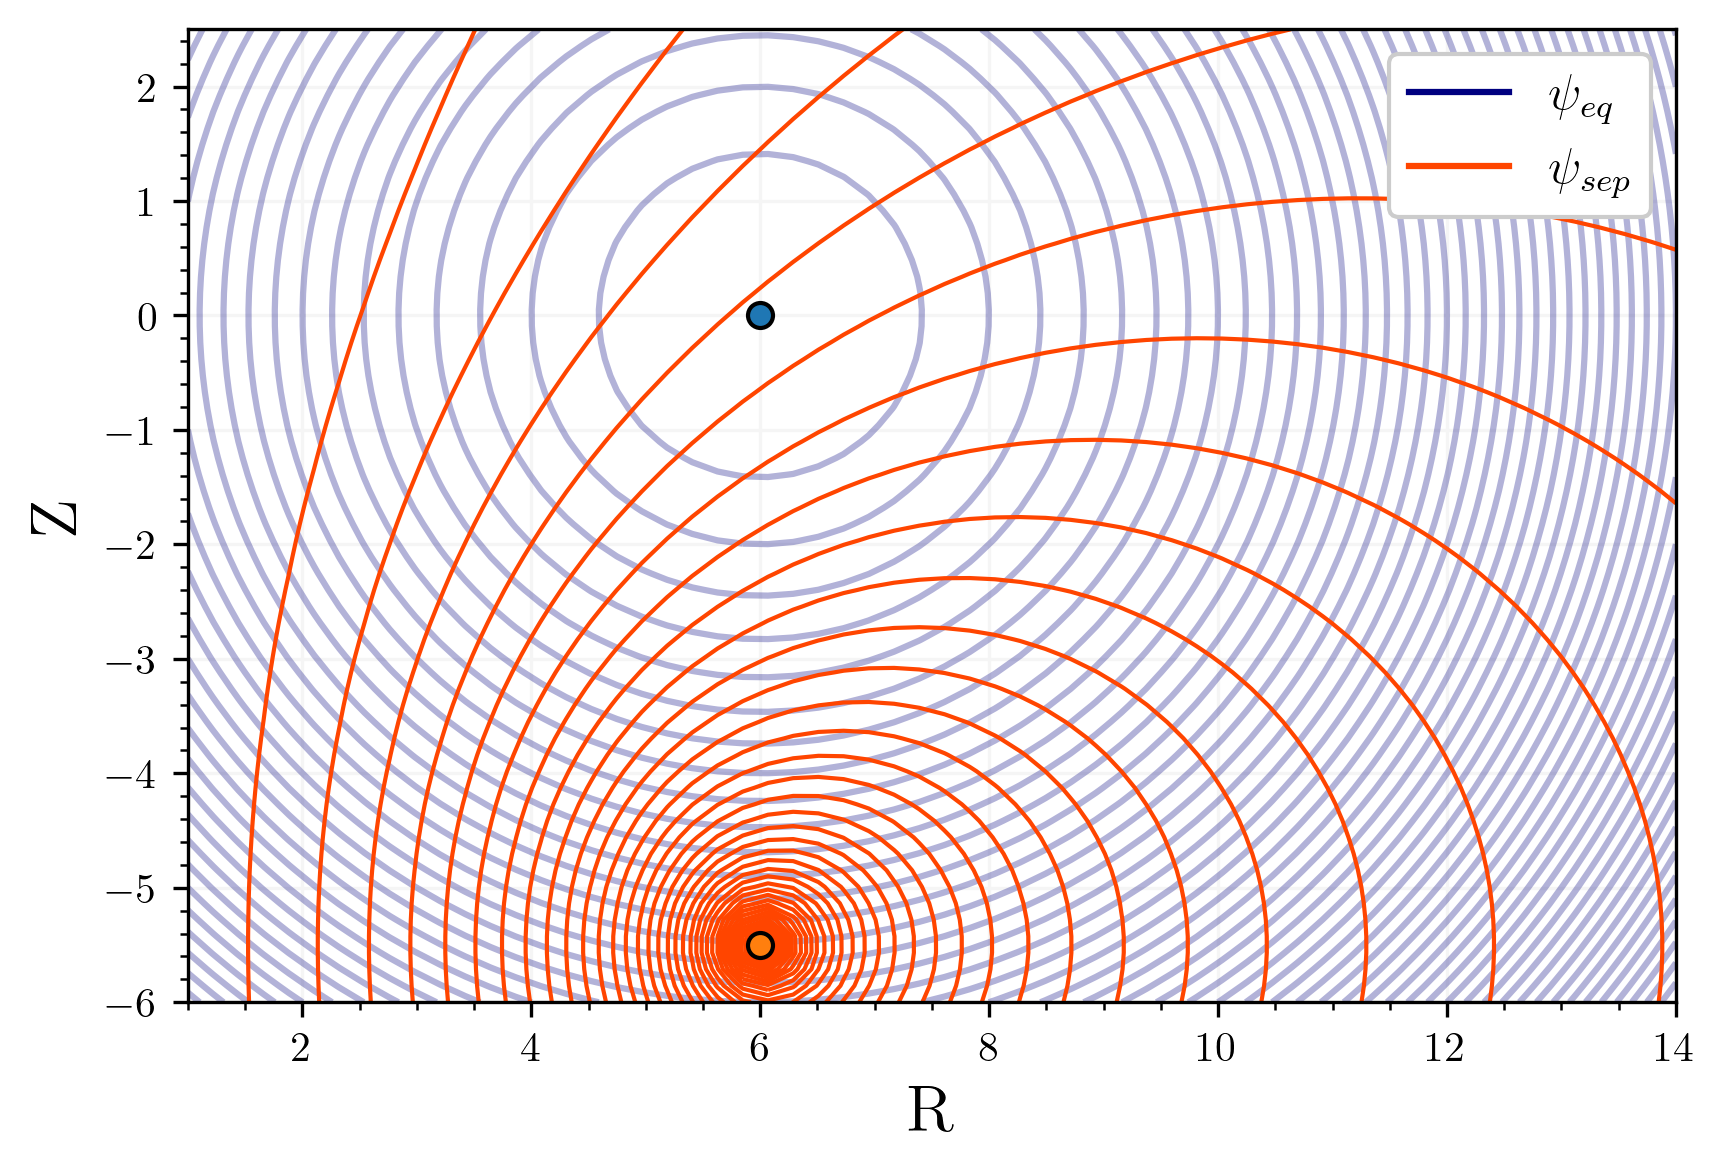
\includegraphics[width=\textwidth]{images/toytok/unperturbed/sepflux.png}
            \caption{}
            \label{fig:toytok-base-psi}
        \end{subfigure}
        \vfill
        \vspace{10px}
        \vfill
        \begin{subfigure}[b]{0.99\textwidth}
            \centering
            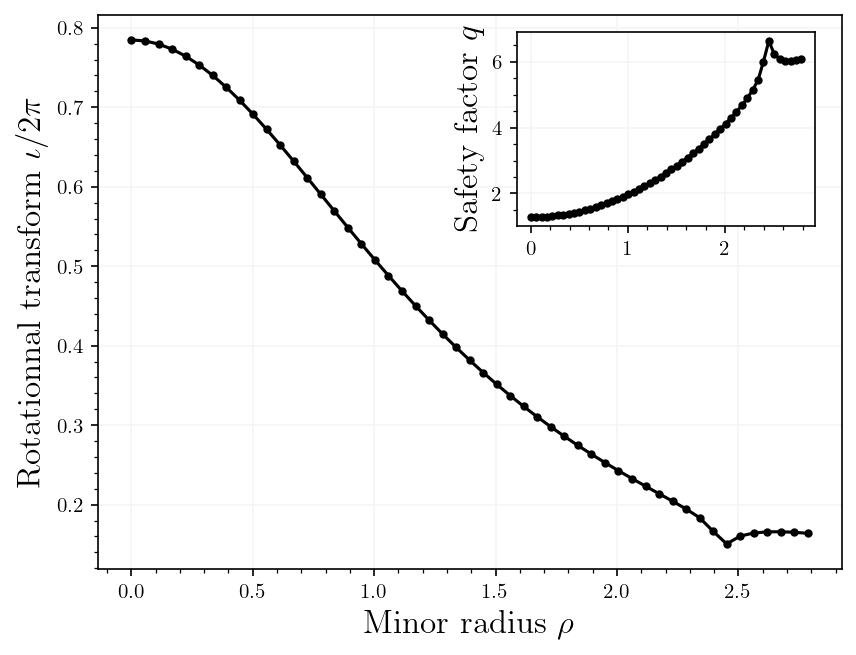
\includegraphics[width=\textwidth]{images/toytok/unperturbed/q-iota-squared.png}
            \caption{}
            \label{fig:toytok-base-iotaq}
        \end{subfigure}
    \end{minipage}%
    \begin{minipage}{0.5\textwidth} % Adjust width as needed
        \centering
        \begin{subfigure}[b]{\textwidth}
            \centering
            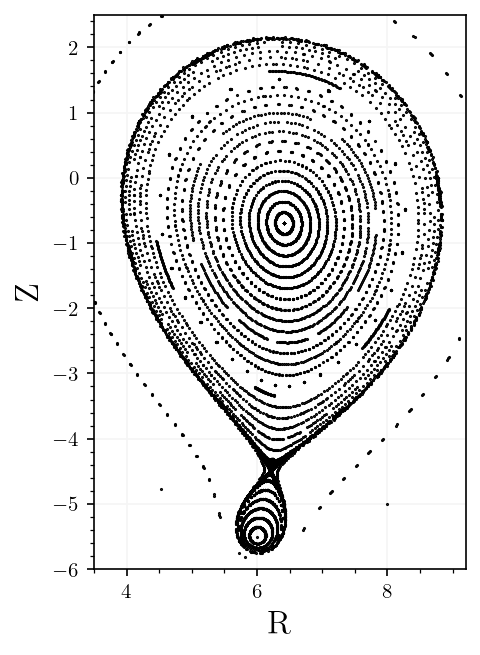
\includegraphics[width=\textwidth]{images/toytok/unperturbed/poincare.png}
            \caption{}
            \label{fig:toytok-base-p}
        \end{subfigure}
    \end{minipage}
    \caption{Analytical Tokamak equilibrium obtained by (a) the addition of the $\psi_{sep}$ function generated by a current loop on top of a high aspect-ratio toroids equilibrium. (b) $\iota/2\pi$ and $q$ profiles and (c) resulting Poincaré section.}
    \label{fig:toytok-base}
\end{figure}

\section{Perturbations}

Since the equilibria generated in the \textit{Toybox} so far are axisymmetric, Noether's theorem implies that there can be only closed flux surfaces and no chaos. To make it appear, perturbations $\delta\textbf{A}$ must be applied. Using simple toroidal coordinates $\phi$, $\theta$ and $0 < \rho < R_\text{max}(\theta)$, makes any function periodic in $\theta$ and $\phi$. Thus one can develop any component of the perturbation into a Fourier series as~:
\begin{align*}
    \delta A^i(\rho,\phi,\theta) = \sum\limits_{n\in\mathbb{N}}\sum\limits_{m\in\mathbb{N}} \delta A^i(\rho)\cos(n\phi + \varphi_n)\cos(m\theta + \varphi_m)
\end{align*}

\cite{escande_description_2024} note that while $\delta\textbf{A}$ generally has 3 components, with a suitable redefinition of the perturbation in straight field line coordinates $\delta\textbf{A}$ can always be of the form $\delta\textbf{A} = -\delta\psi \nabla\phi$ with only a $\phi$ component. Although $\rho$ and $\theta$ are generally not straight field line coordinates, using the same approach, writing $\psi_\text{pert} = R^2\delta A^\phi$ and taking only one Fourier mode pair $(m,n)$ will provide the building block for the toybox perturbations.

The resonant surface has a specific $q$ value and can be targeted, but applying the perturbation to a more widespread region was thought to be more effective and somewhat realistic. For the radial profile of $\psi_{pert}$,  $f(\rho) = R^2\delta A^\phi(\rho)$, the Normal and Maxwell-Boltzmann distribution are implemented~:
\begin{enumerate}
    \item A Normal distribution $f(\rho, \mu, \sigma) = \frac{1}{\sqrt{2\pi\sigma^2}}\exp\left(\frac{-(\rho-\mu)^2}{2\sigma^2}\right)$ with mean  and mode $\mu$ and variance $\sigma^2$.
    \item A Maxwell-Boltzmann distribution $f(\rho, d) = \frac{\sqrt{2}}{\sqrt{\pi}}\frac{\rho^2}{d^3}\exp\left(\frac{-\rho^2}{2d^2}\right)$ with mean $a$, mode, and variance $a$.
\end{enumerate}
\newcommand{\amp}{\varepsilon_\text{amp}}
The last parameter that can be select in this implementation is the amplitude $\amp$ of the linear combination $\textbf{A} + \amp\delta\textbf{A}$. A fair way to compare the perturbations, for example by their magnetic energy, could be investigated, but is currently lacking.

First we apply a Maxwell-Boltzmann distributed perturbation to the high aspect ratio equilibrium with the mode pair $m=3$, $n=2$ and to target the $q = 3/2$ surface we set $d = \rho/\sqrt{2}$ and $\amp = 0.1$. The resulting perturbation flux $\psi_\text{pert}$ is shown in \figref{fig:toyha-32-psi}. The more yellow the more $\psi_{pert}$ is  positive and the more purple the more negative. The perturbed magnetic field at $\rho=1.75$ is shown, it follows the curves of the constant $\psi_{pert}$. For the divergence-free condition to be satisfied, the flux/field intensity must be higher on the inside, which is indeed observed. \figref{fig:toyha-32-p} shows the resulting poincare section obtained. The crossings of the $q = 3/2$ island are clearly visible. There also seems to be one island closer to the axis and one outside.

\begin{figure}[H]
    \centering
    \begin{subfigure}[t]{0.55\textwidth}
        \centering
        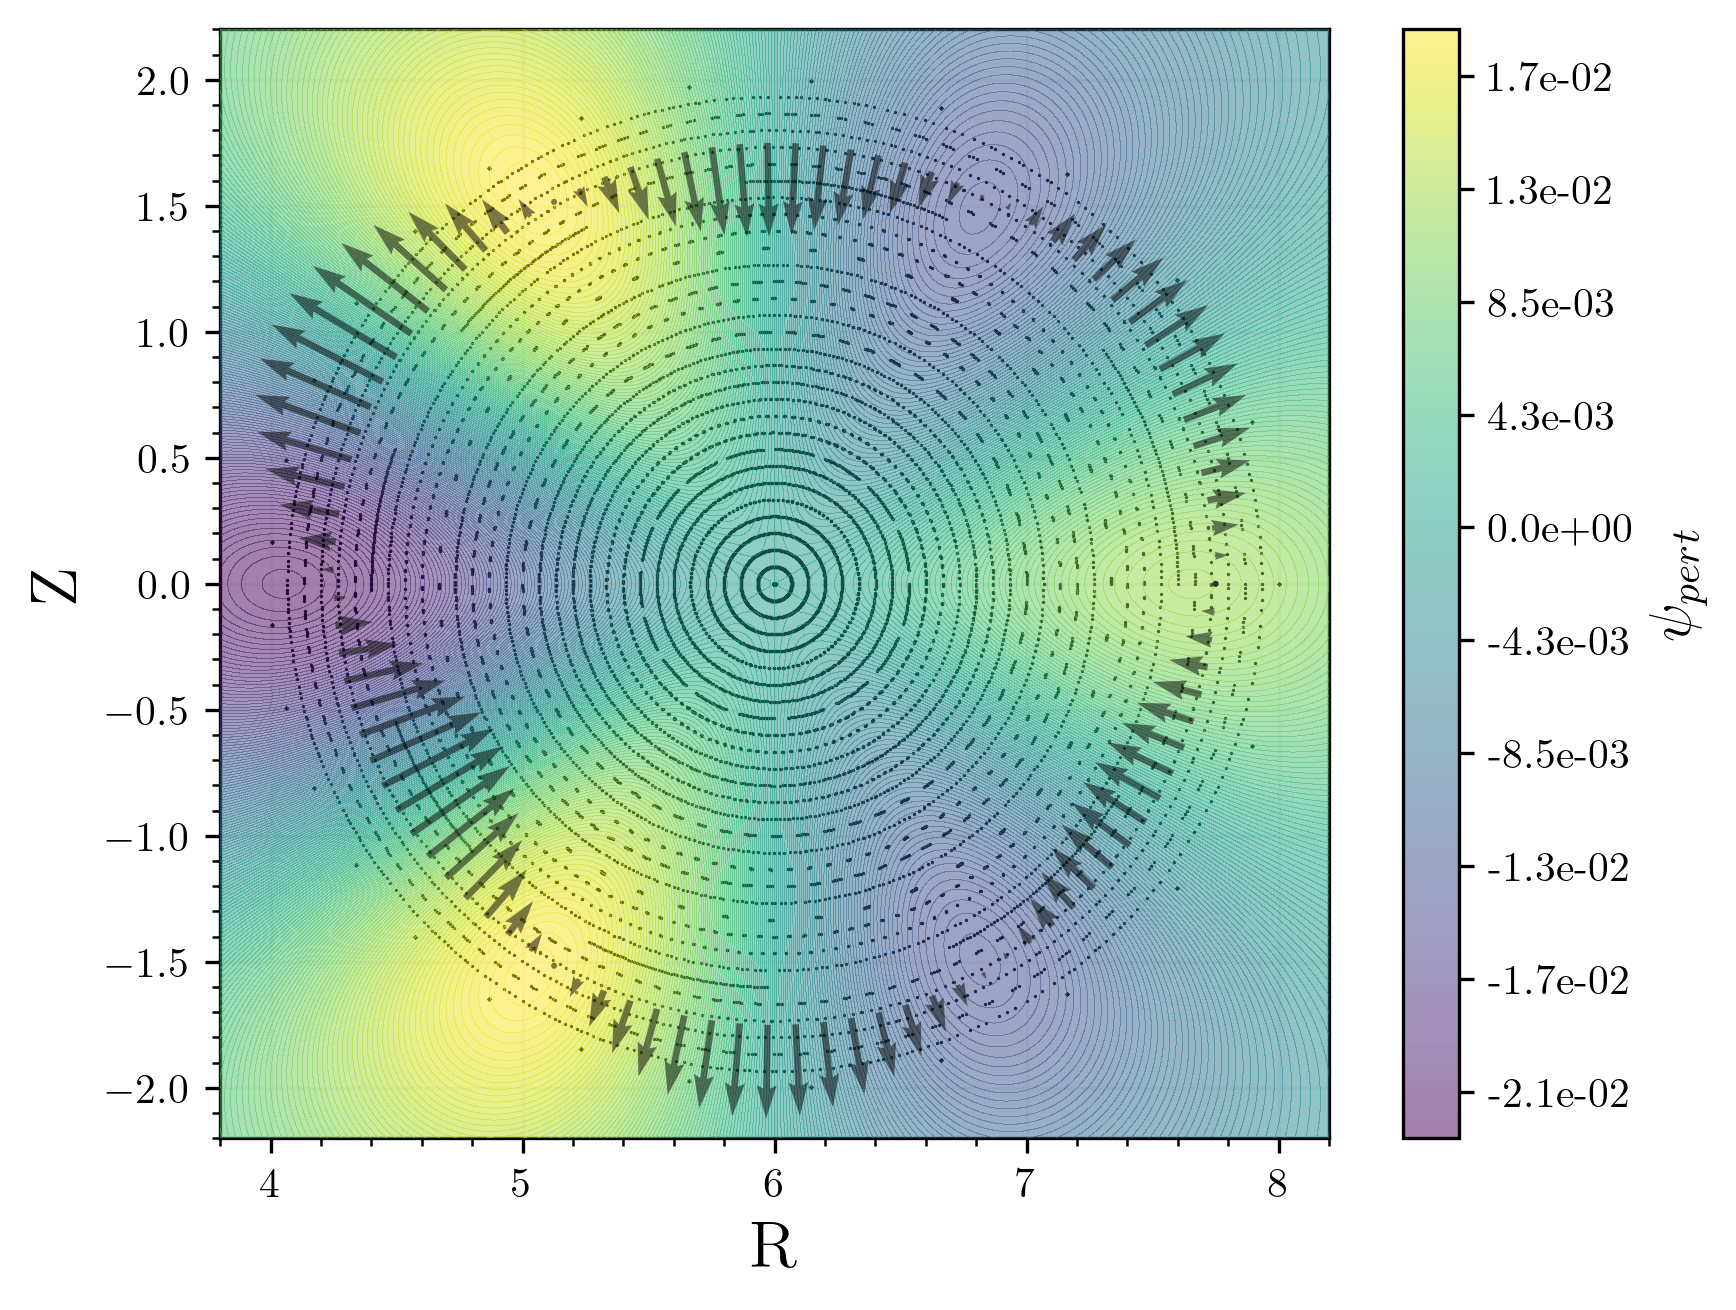
\includegraphics[width=\textwidth]{images/high-aspect-ratio/psi_pert.png}
        \caption{}
        \label{fig:toyha-32-psi}
    \end{subfigure}
    \hfill
    \begin{subfigure}[t]{0.43\textwidth}
        \centering
        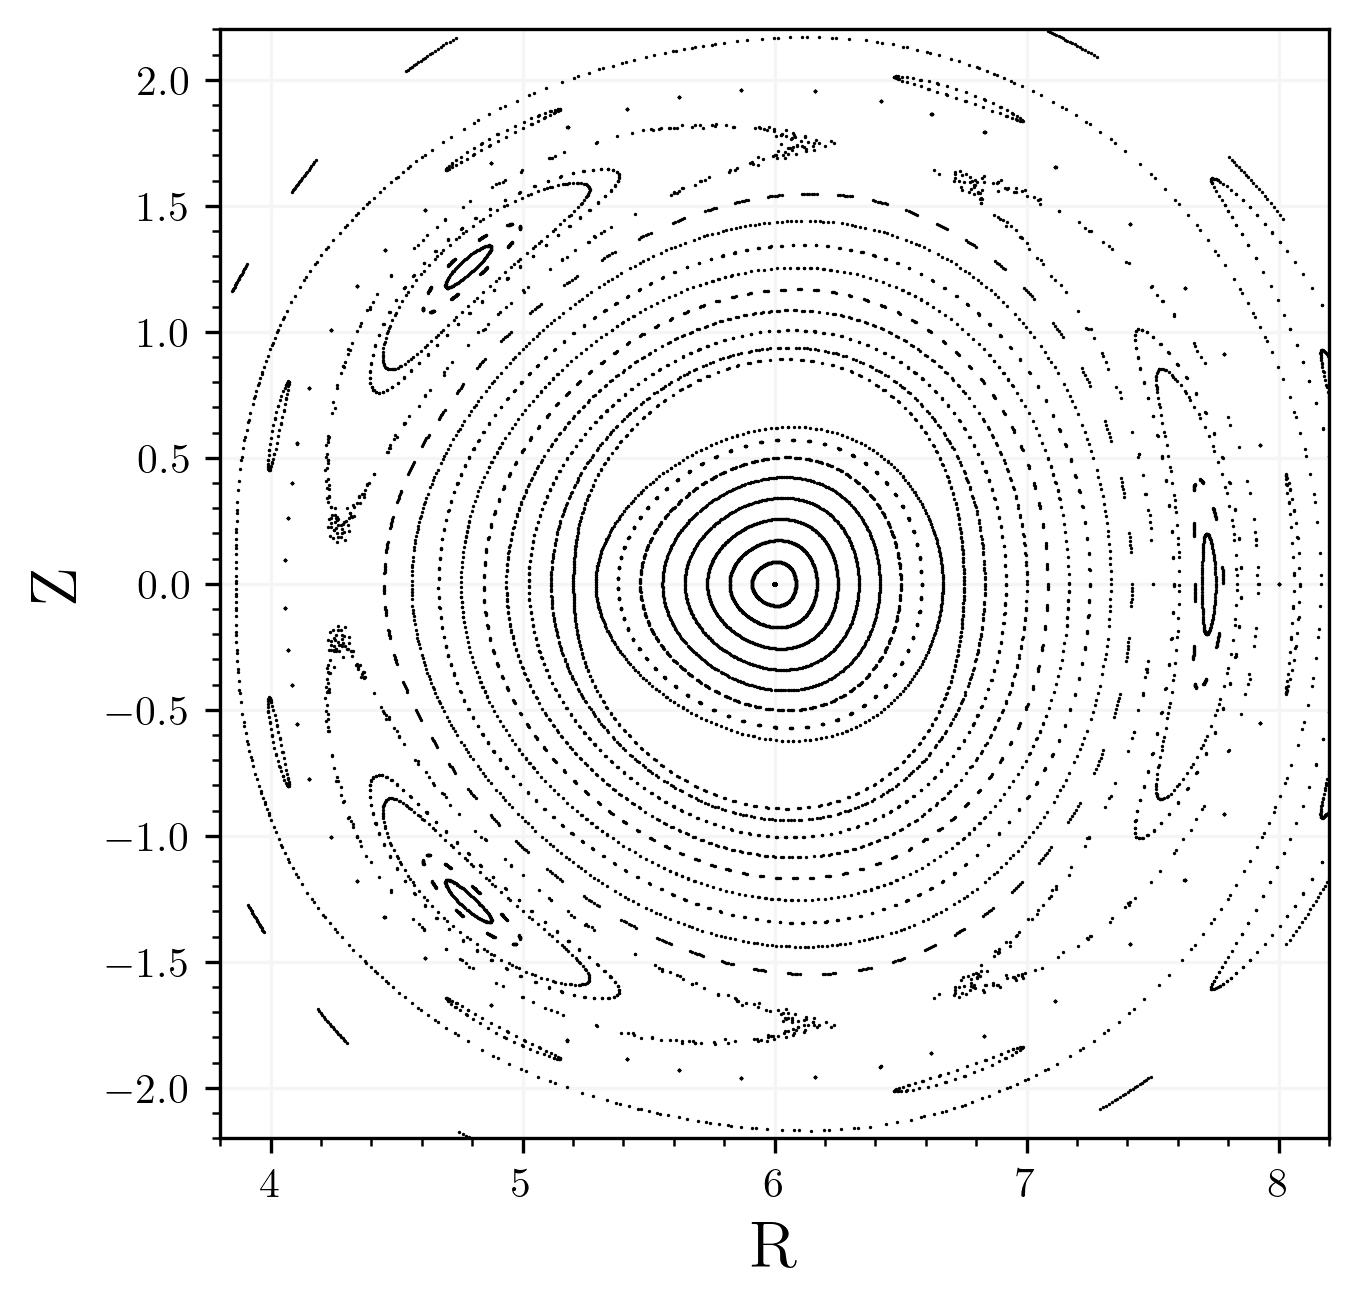
\includegraphics[width=\textwidth]{images/high-aspect-ratio/perturbed_3_2.png}
        \caption{}
        \label{fig:toyha-32-p}
    \end{subfigure}
    \caption{High aspect ratio Tokamak equilibrium perturbed with Maxwell-Boltzmann distributed perturbation $m/n = 3/2$, $d = 1.75/\sqrt{2}$ and $\amp = 0.1$. In (a) the contour of the perturbed flux $\psi_\text{pert}$ and the resulting perturbed field on the $\rho=1.75$ circle. In (b) Poincaré section at $\phi = 0$ for the perturbed magnetic configuration and the 3 crossing of the island.}
    \label{fig:toyha-32}
\end{figure}

While the resulting perturbed high aspect configuration does not appear chaotic at first, we will further see that there is indeed chaos here. In fact the modes of perturbation are not only the $m$ and $n$ which are used in the implementation because the toroidal coordinates are not straight field line coordinates. \figref{fig:mode-mixing} shows the angle between the $B^\phi\partial_\phi$ and $\textbf{B}$ obtained by the $\arctan(B^\theta/B^\phi)$ with respect to the angle position $\theta$, $\phi$ on the $\rho = 1.75$ surface in the case of the unperturbed high aspect ratio equilibrium. The highest values are more red and indicate that the field is more oriented towards $\partial_\phi$. Lower values are shown in blue. The angle changes with $\theta$, which is not the case for straight field line coordinates\footnote{The basis transformation can be found for example in \cite[p.116]{dhaeseleer_flux_1991}.}, where it would be constant and equal to $\iotaslash(\rho) = 2/3$. This distinction introduces mode mixing, the initial delta distribution in Fourier space is broadened and thus chaos appears faster, which is a welcome feature in this case.

\begin{figure}[H]
    \centering
    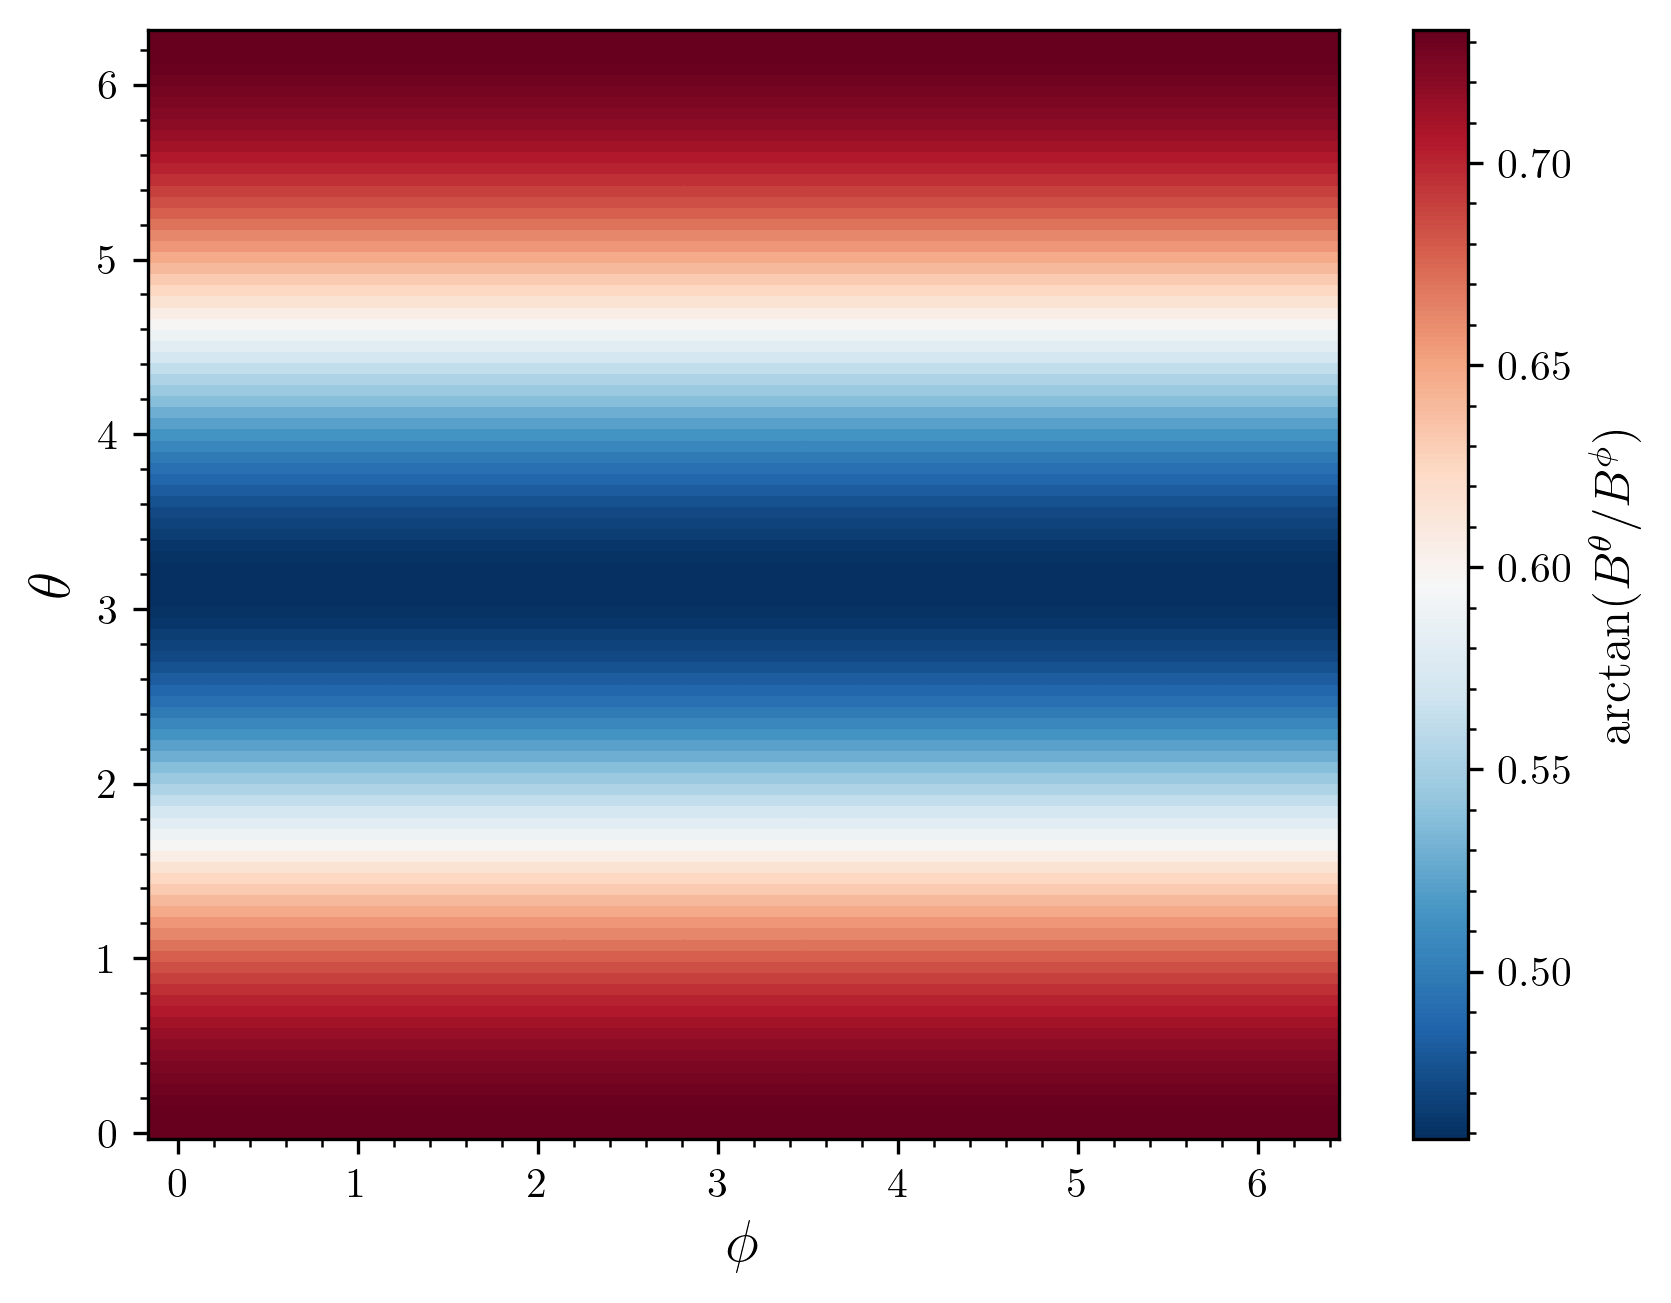
\includegraphics[width=0.7\textwidth]{images/high-aspect-ratio/fieldlines.png}
    \caption{Angle between $B^\phi\partial_\phi$ and $\textbf{B}$ in radian against the poloidal $\theta$ and toroidal $\phi$ angles for the magnetic surface at $\rho = 1.75$ and with $q(\rho) = 3/2$.}
    \label{fig:mode-mixing}
\end{figure}

A Maxwell-Boltzmann distributed perturbation can also be added to the single null Tokamak equilibrium. Checking the safety factor profile \figref{fig:toytok-base-iotaq} suggest picking a pair of modes $m=6$, $n=1$ and $d = \sqrt{2}$ (to target $\rho = 2$) and $\amp = 0.1$. Similar to the high aspect ratio case, the \figref{fig:toytok-61-psi} shows the $\psi_\text{pert}$ over the single null tokamak equilibrium. The orientation changes from pointing inward to outward 12 times. The Poincaré section of the resulting field is shown in figure \figref{fig:toytok-61-p}.

The regime can be here seen to be chaotic and there are many islands/island chains. A set of points starting close to the X-point make a more dense layer on the position of the previous separatrix. The position of the O-point is not affected by the perturbation and the X-point is shifted by a relative change of order $10^{-3}$. A closer look at the field lines around the X-point is shown in \figref{fig:xpoint-chaos} with different colours for each field line and the X-point as a crossed marker. It reveals how the field lines are mix in this region. Some higher order islands are also discovered. 

\begin{figure}
    \centering
    \begin{subfigure}{0.57\textwidth}
        \centering
        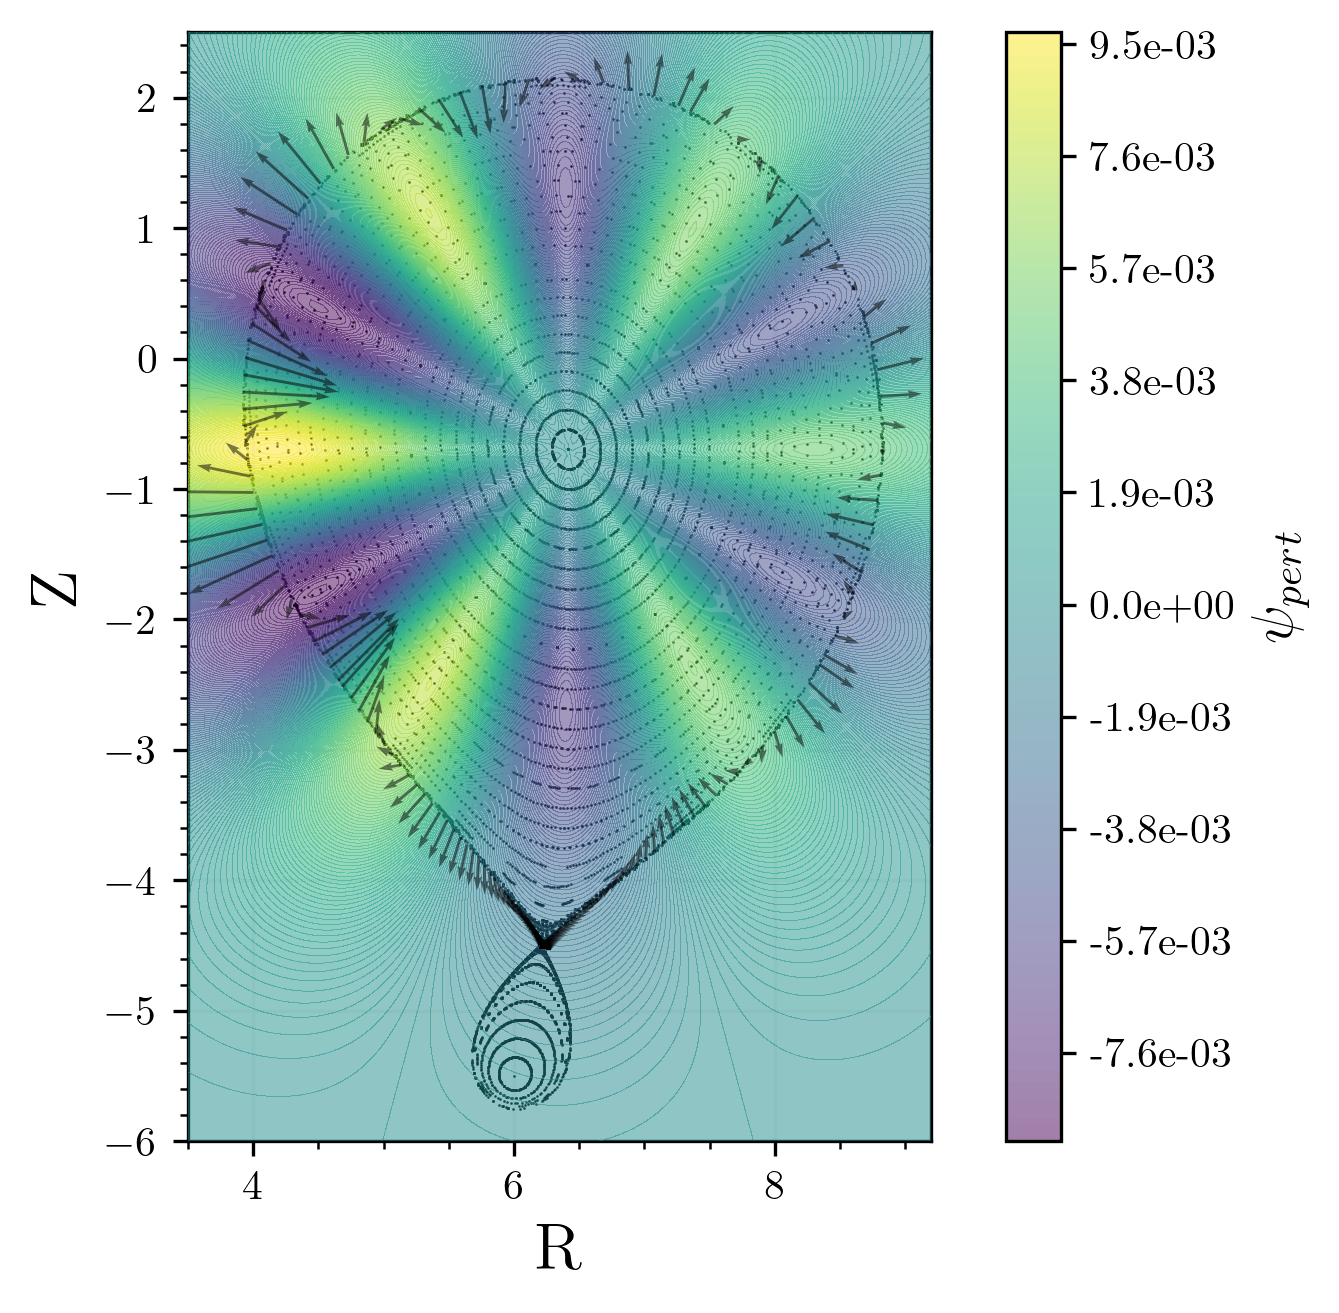
\includegraphics[width=\textwidth]{images/toytok/perturbed-6-1/psi_pert.png}
        \caption{}
        \label{fig:toytok-61-psi}
    \end{subfigure}
    \hfill
    \begin{subfigure}{0.41\textwidth}
        \centering
        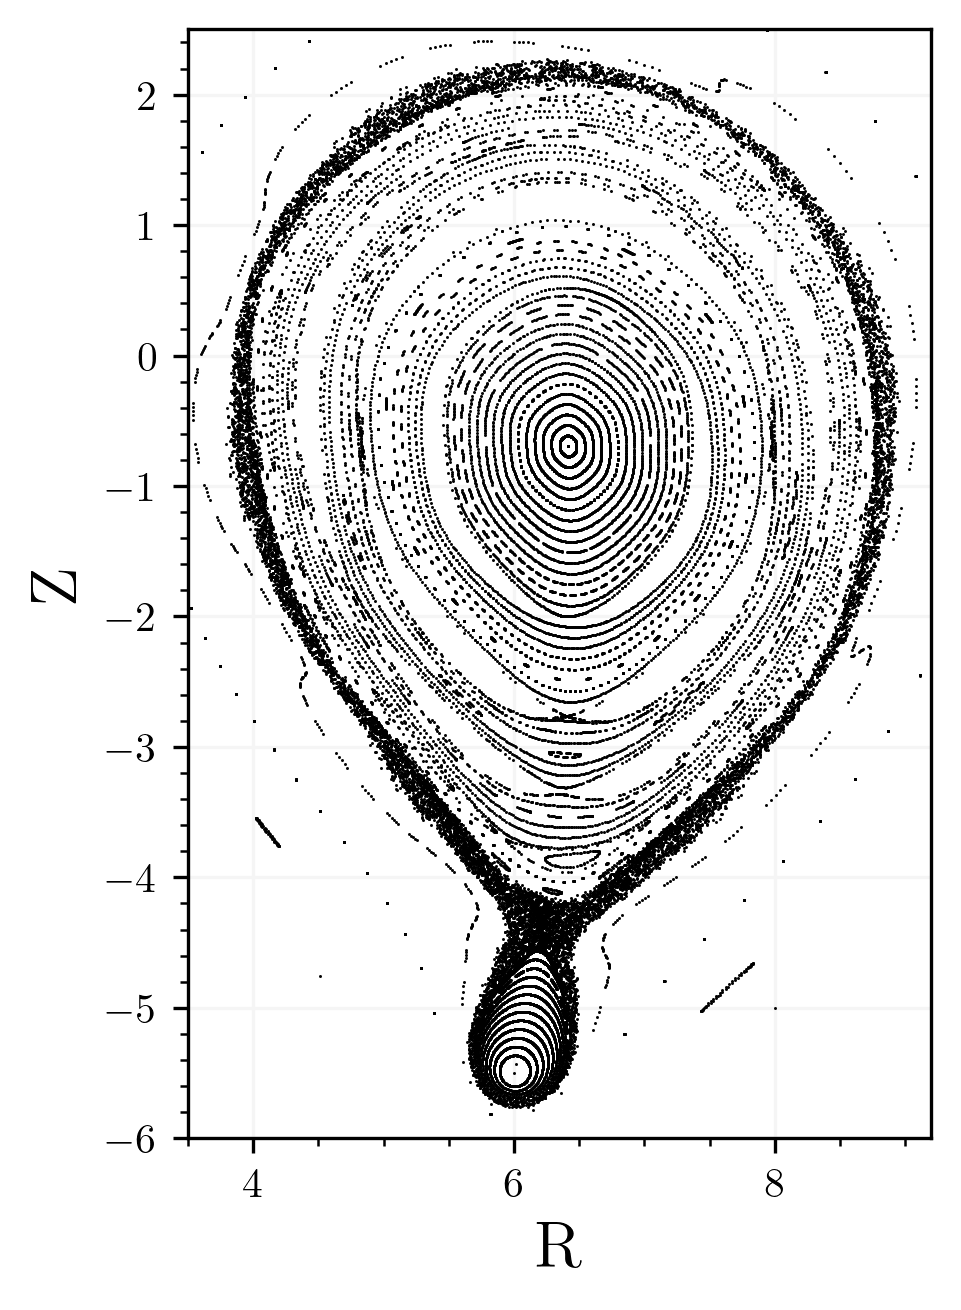
\includegraphics[width=\textwidth]{images/toytok/perturbed-6-1/perturbed_6_1.png}
        \caption{}
        \label{fig:toytok-61-p}
    \end{subfigure}
    \caption{Single null Tokamak equilibrium perturbed with Maxwell-Boltzmann distributed perturbation $m/n = 6/1$, $d = \sqrt{2}$ and $\amp = 0.1$. In (a) the contour of the perturbed flux $\psi_\text{pert}$ and the resulting perturbed field on the unperturbed separatrix. In (b) Poincaré section at $\phi = 0$ for the perturbed magnetic configuration.}
    \label{fig:toytok-61}
\end{figure}

\begin{figure}
    \centering
    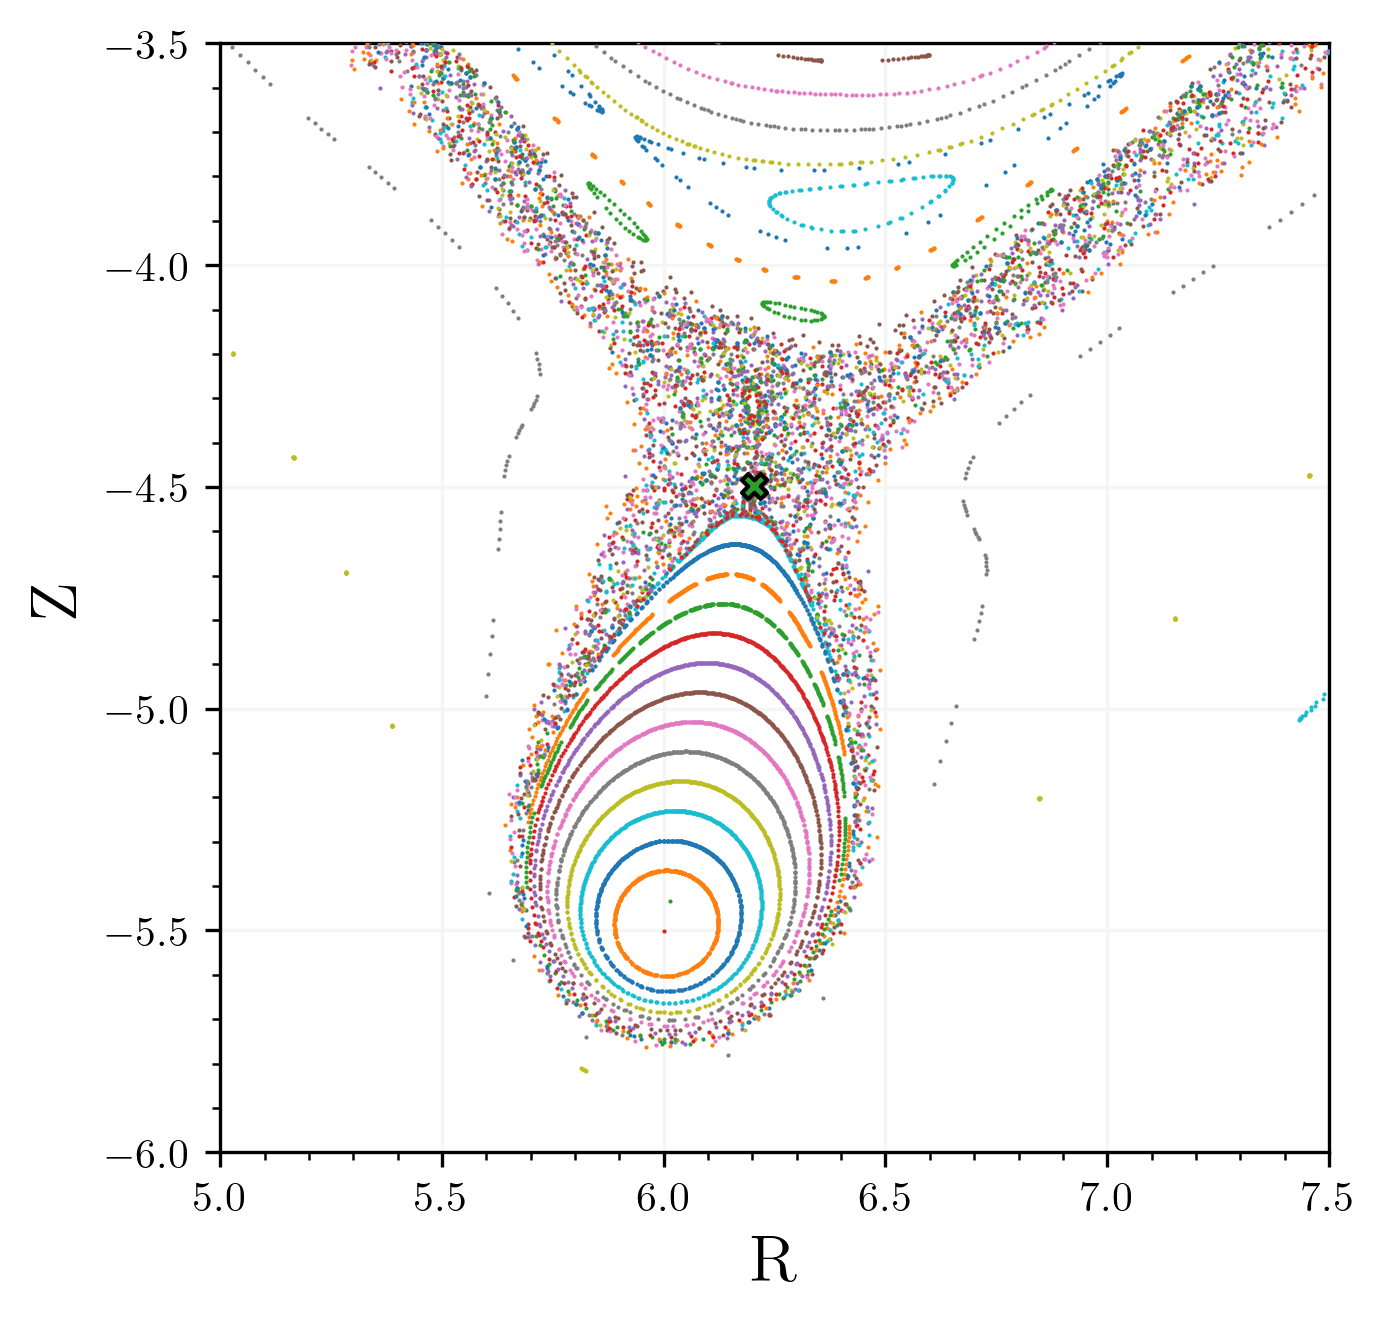
\includegraphics[width=0.5\textwidth]{images/toytok/perturbed-6-1/perturbed_6_1_closer.png}
    \caption{Zoom in view around the X-point of the single null Tokamak equilibrium showing the chaotic behaviour of the nearby field line.}
    \label{fig:xpoint-chaos}
\end{figure}

\chapter{Tangles and Turnstiles}\label{ch:tangleandturns}

Hamiltonian dynamical systems may display some dependency on the initial position. Such that starting point that are indistinguishably close at time $t_0$ give completely different outcome, and while the system is deterministic !

This was often put in word as the butterfly effect, a flap in the winds of a butterfly at the end other end of the world can change the initial state enough so that the end result is a, let's not wish us bad things, a snow storm happening or not.\footnote{A really nice book to read about chaos is James Gleick.}

This seemingly erratic behaviour is however structured with the apparition of ever repeating pattern, zooming and zooming and. Some progress beautiful math is at the core of chaos, KAM theory.

In the fusion research, the fact to follow the field line is such a hamiltonian \cite{escande_description_2024}\cite{abdullaev_magnetic_2014}\cite{viana_hamiltonian_2023} system that often is prone to chaos. This can be a feature or a bug depending on the configuration. 

A measure of transport due to chaos is \cite{meiss_thirty_2015} which works in the more general case of volume-preserving maps. The transport is measured by exit and entry fluxes. For area-preserving maps, transport is impeded by invariant manifolds forming partial barriers. For exact volume-preserving maps, flux computation reduces to finding the difference between the actions of key orbits, such as homoclinic orbits to a saddle or cantorus. More mathy definition about the Floer homology, can be found in well \cite{hohloch_transport_2012}\cite{hohloch_homoclinic_2017}. He make the point that  characterisation of transport in deterministic dynamical systems involves the computation of exit and transition time distributions in phase space. 

The resulting idea is that there are partial barriers formed by two curve and forming a infinite grid structure which, a link to the fractal. This structre now often called tangles were first studied by H. Poincare in the three body problem of celestial mechanics \cite{poincare_methodes_1899}. He used to called them trellis as the interconnection formed resemble such a strange object.

The study of tangle and turnstiles in the case of the field line map will be part of the \href{https://github.com/zhisong/pyoculus}{\textcolor{blue}{\textit{Pyoculus}}} package.

It will hopefully be a strong foundation toolkit to look into the chaos : to strengthen the understanding of the in of chaotic systems.

\section{Stable and Unstable Manifolds}\label{sec:manif}

The exponential behaviour along the stable and unstable directions, given by the stable $\textbf{e}_s$ and unstable $\textbf{e}_u$ eigenvectors, of a saddle fixed point $x^\star$ can be expressed by stating that for small $\varepsilon$ the points $x = x^\star + \varepsilon\,\textbf{e}_s$ will converge to $x^\star$ as we apply $\pmap$ and the points $x = x^\star + \varepsilon\,\textbf{e}_s$ converge to $x^\star$ as we apply $\pmap^{-1}$. More specifically, the stable manifold $W^s(x_s^\star)$ is defined as the set for which $\pmap^k(x)\to x_s^\star$ as $k\to\infty$. Similarly, the unstable manifold $W^u(x_u^\star)$ is the set of points such that $\pmap^k(x)\to x_u^\star$ as $k\to -\infty$. This definition includes not only the points in the linear regime, but also the points forming their trajectory. In the following, the manifolds are just written as $W^s$ and $W^u$ both when $x_s^\star = x_u^\star$ and when it is not.

In the case of a two dimensional map, such as $\pmap$, the stable manifold theorem proves that there exist immersions $\gamma_u$ and $\gamma_s$ mapping $\mathbb{R}$ to $W^s$ and $W^u$ with $\gamma_s(0) = \gamma_u(0) = x^\star$ \cite{easton_trellises_1986}. It implies that the point on the stable and unstable manifold can be ordered by inducing the order of $\mathbb{R}$, yielding the stable and unstable orderings $>_s$ and $>_u$. The four components $W_+^s$, $W_-^s$, $W_+^u$ and $W_-^u$ correspond to the orientations $\pm\textbf{e}_s$, $\pm\textbf{e}_u$ and to the mapping of $\mathbb{R}^+$, $\mathbb{R}^-$ through $\gamma_s$ and $\gamma_u$.

Each of the four components, for example $W^s_+$, can then be described by picking $q \in W^s_+$ and considering the initial segment $S^+ = ]q,\pmap(q)]_s \subset W^s_+$. By applying $\pmap$ and $\pmap^{-1}$ to $S^+$ for a sufficient number of iterations, it is possible to recover any part of the component.

For a single null tokamak equilibrium, the separatrix consists of two components $W^s_+ = W^u_+$. They are in principle 3-dimensional, but again, since their evolution is continuous in $\phi$, their 2-dimensional intersection with a phi-plane is considered. In the chaotic case, $W^s_+$ and $W^u_-$ are no longer equal. A simple algorithm to draw them out then consists to follow the evolution of an initial segment $S^+$ and $U^+$.

\begin{figure}[H]
    \centering
    \begin{minipage}{0.45\textwidth} % Adjust width as needed
        \centering
        \begin{subfigure}[b]{\textwidth}
            \centering
            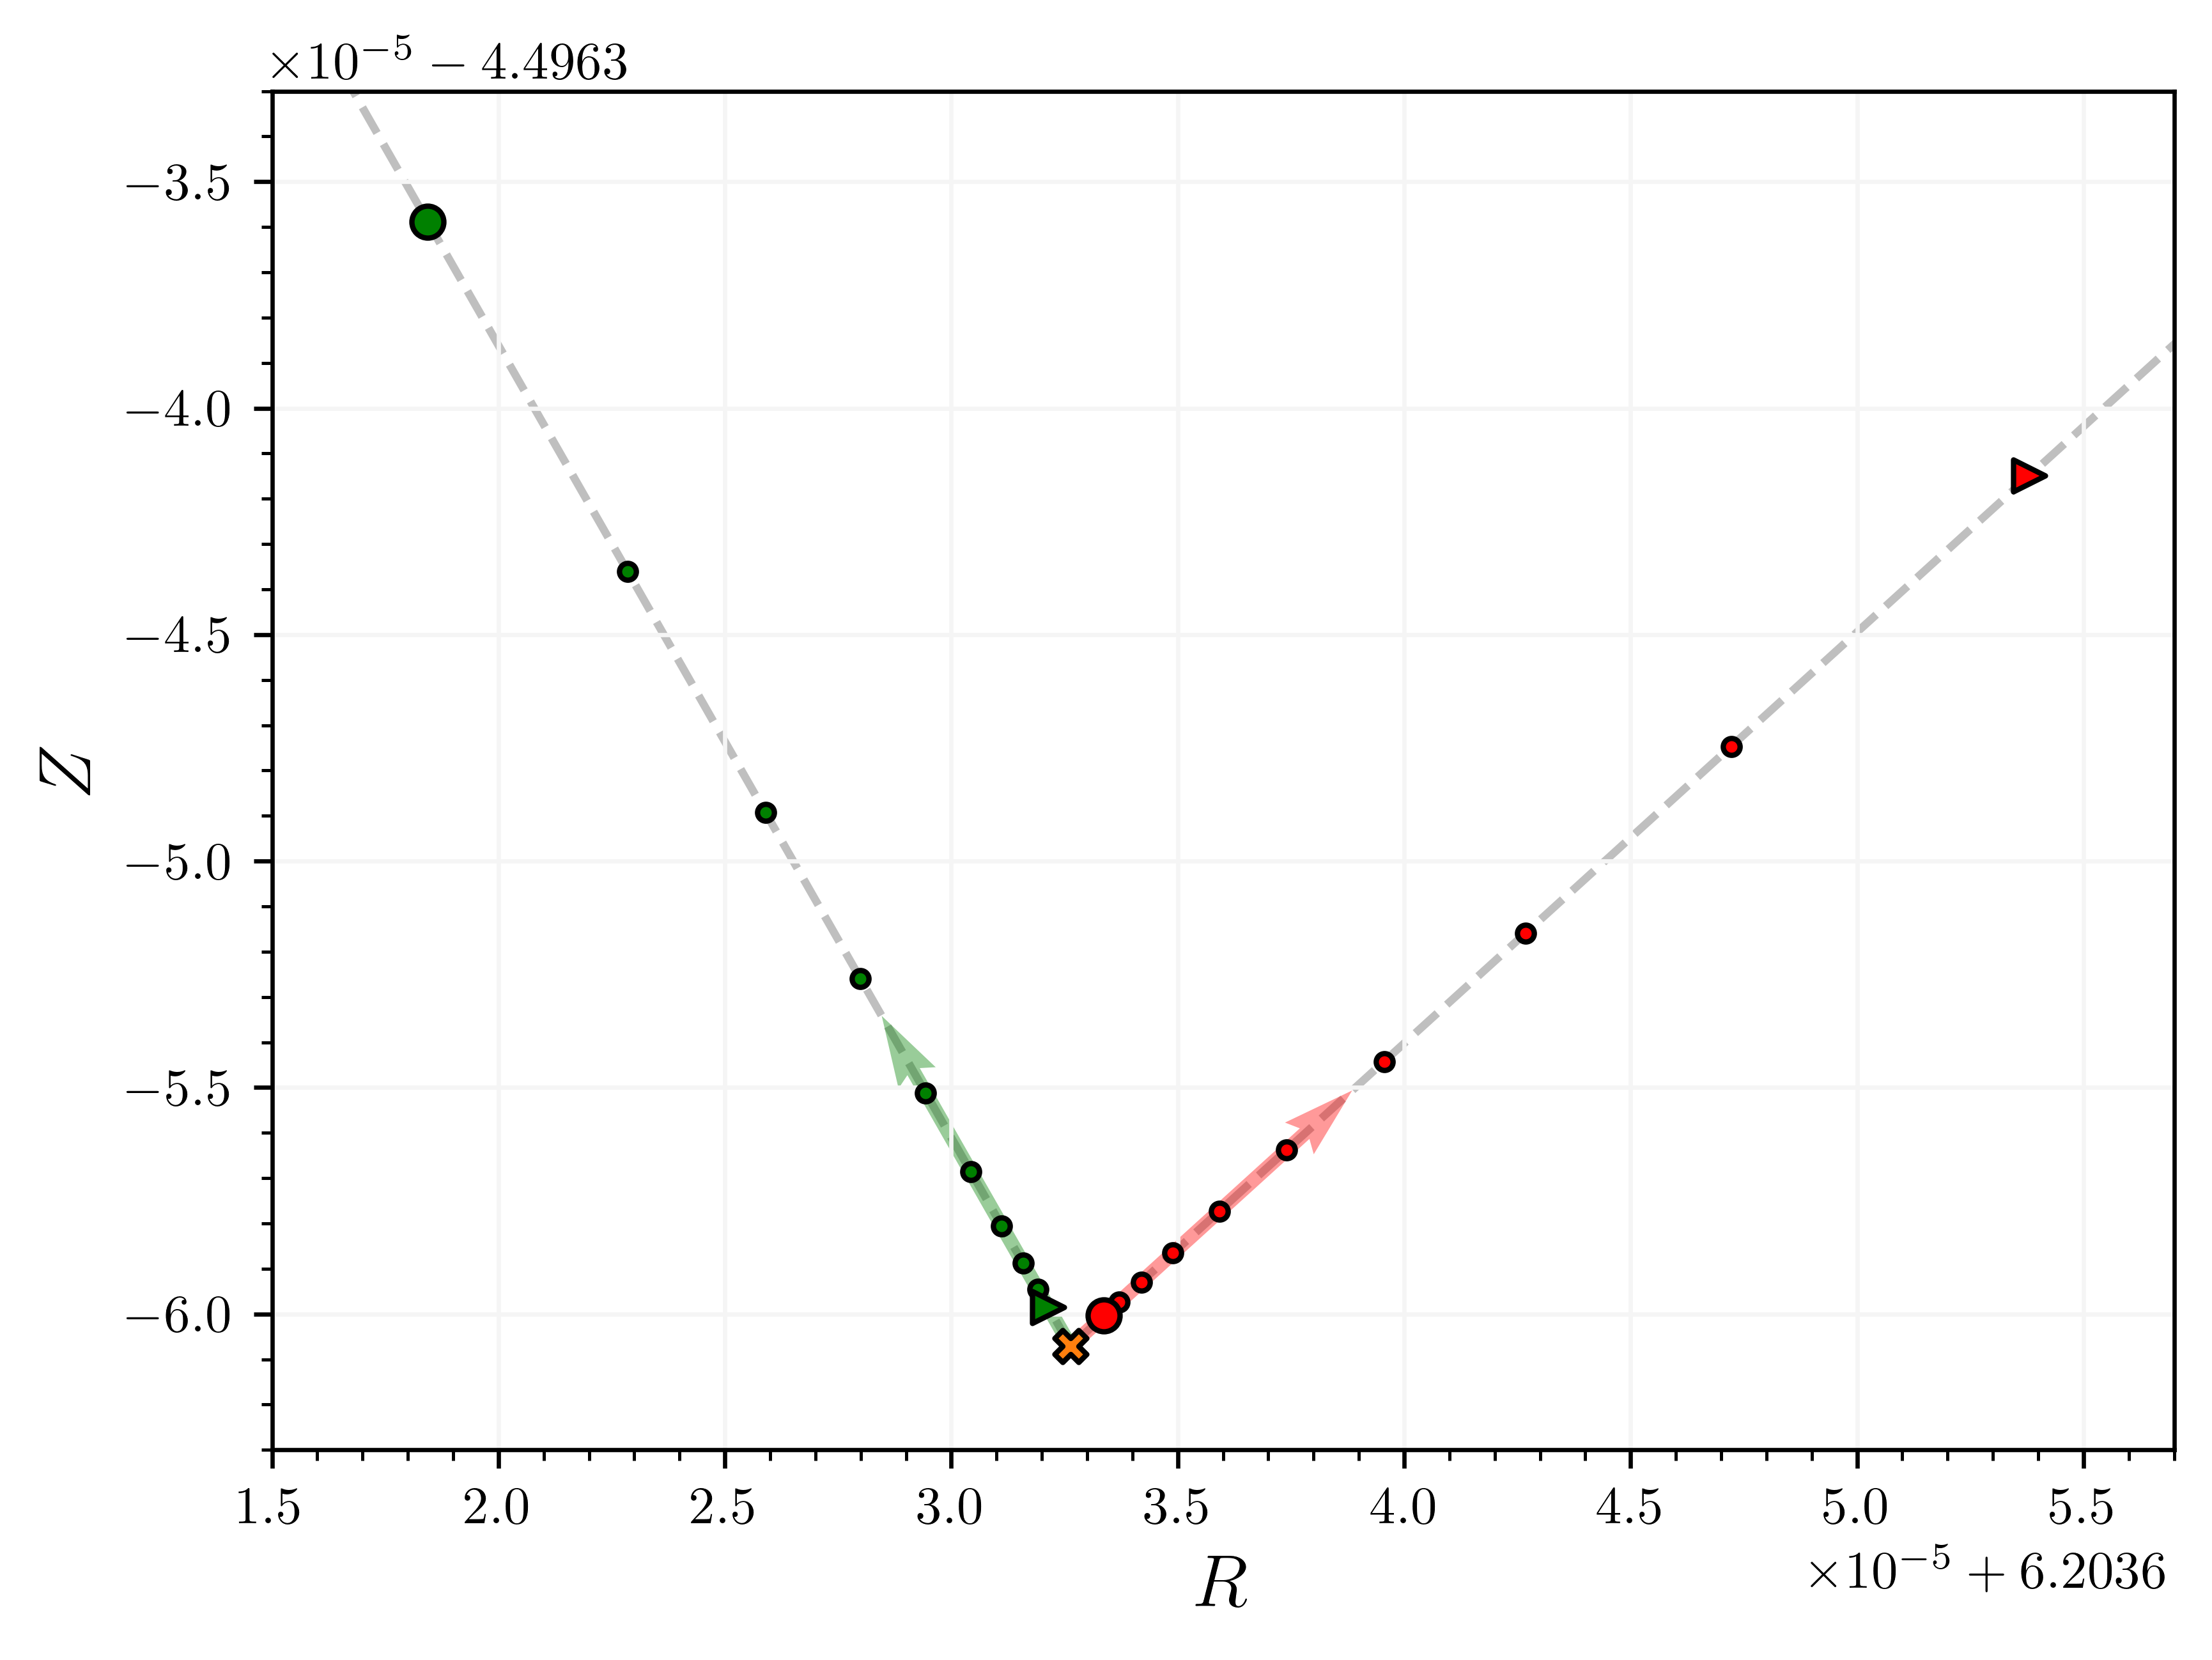
\includegraphics[width=\textwidth]{images/manifold/manifold_start.png}
            \caption{}
            \label{fig:man-a}
        \end{subfigure}
        \vfill
        \vspace{10px}
        \vfill
        \begin{subfigure}[b]{0.99\textwidth}
            \centering
            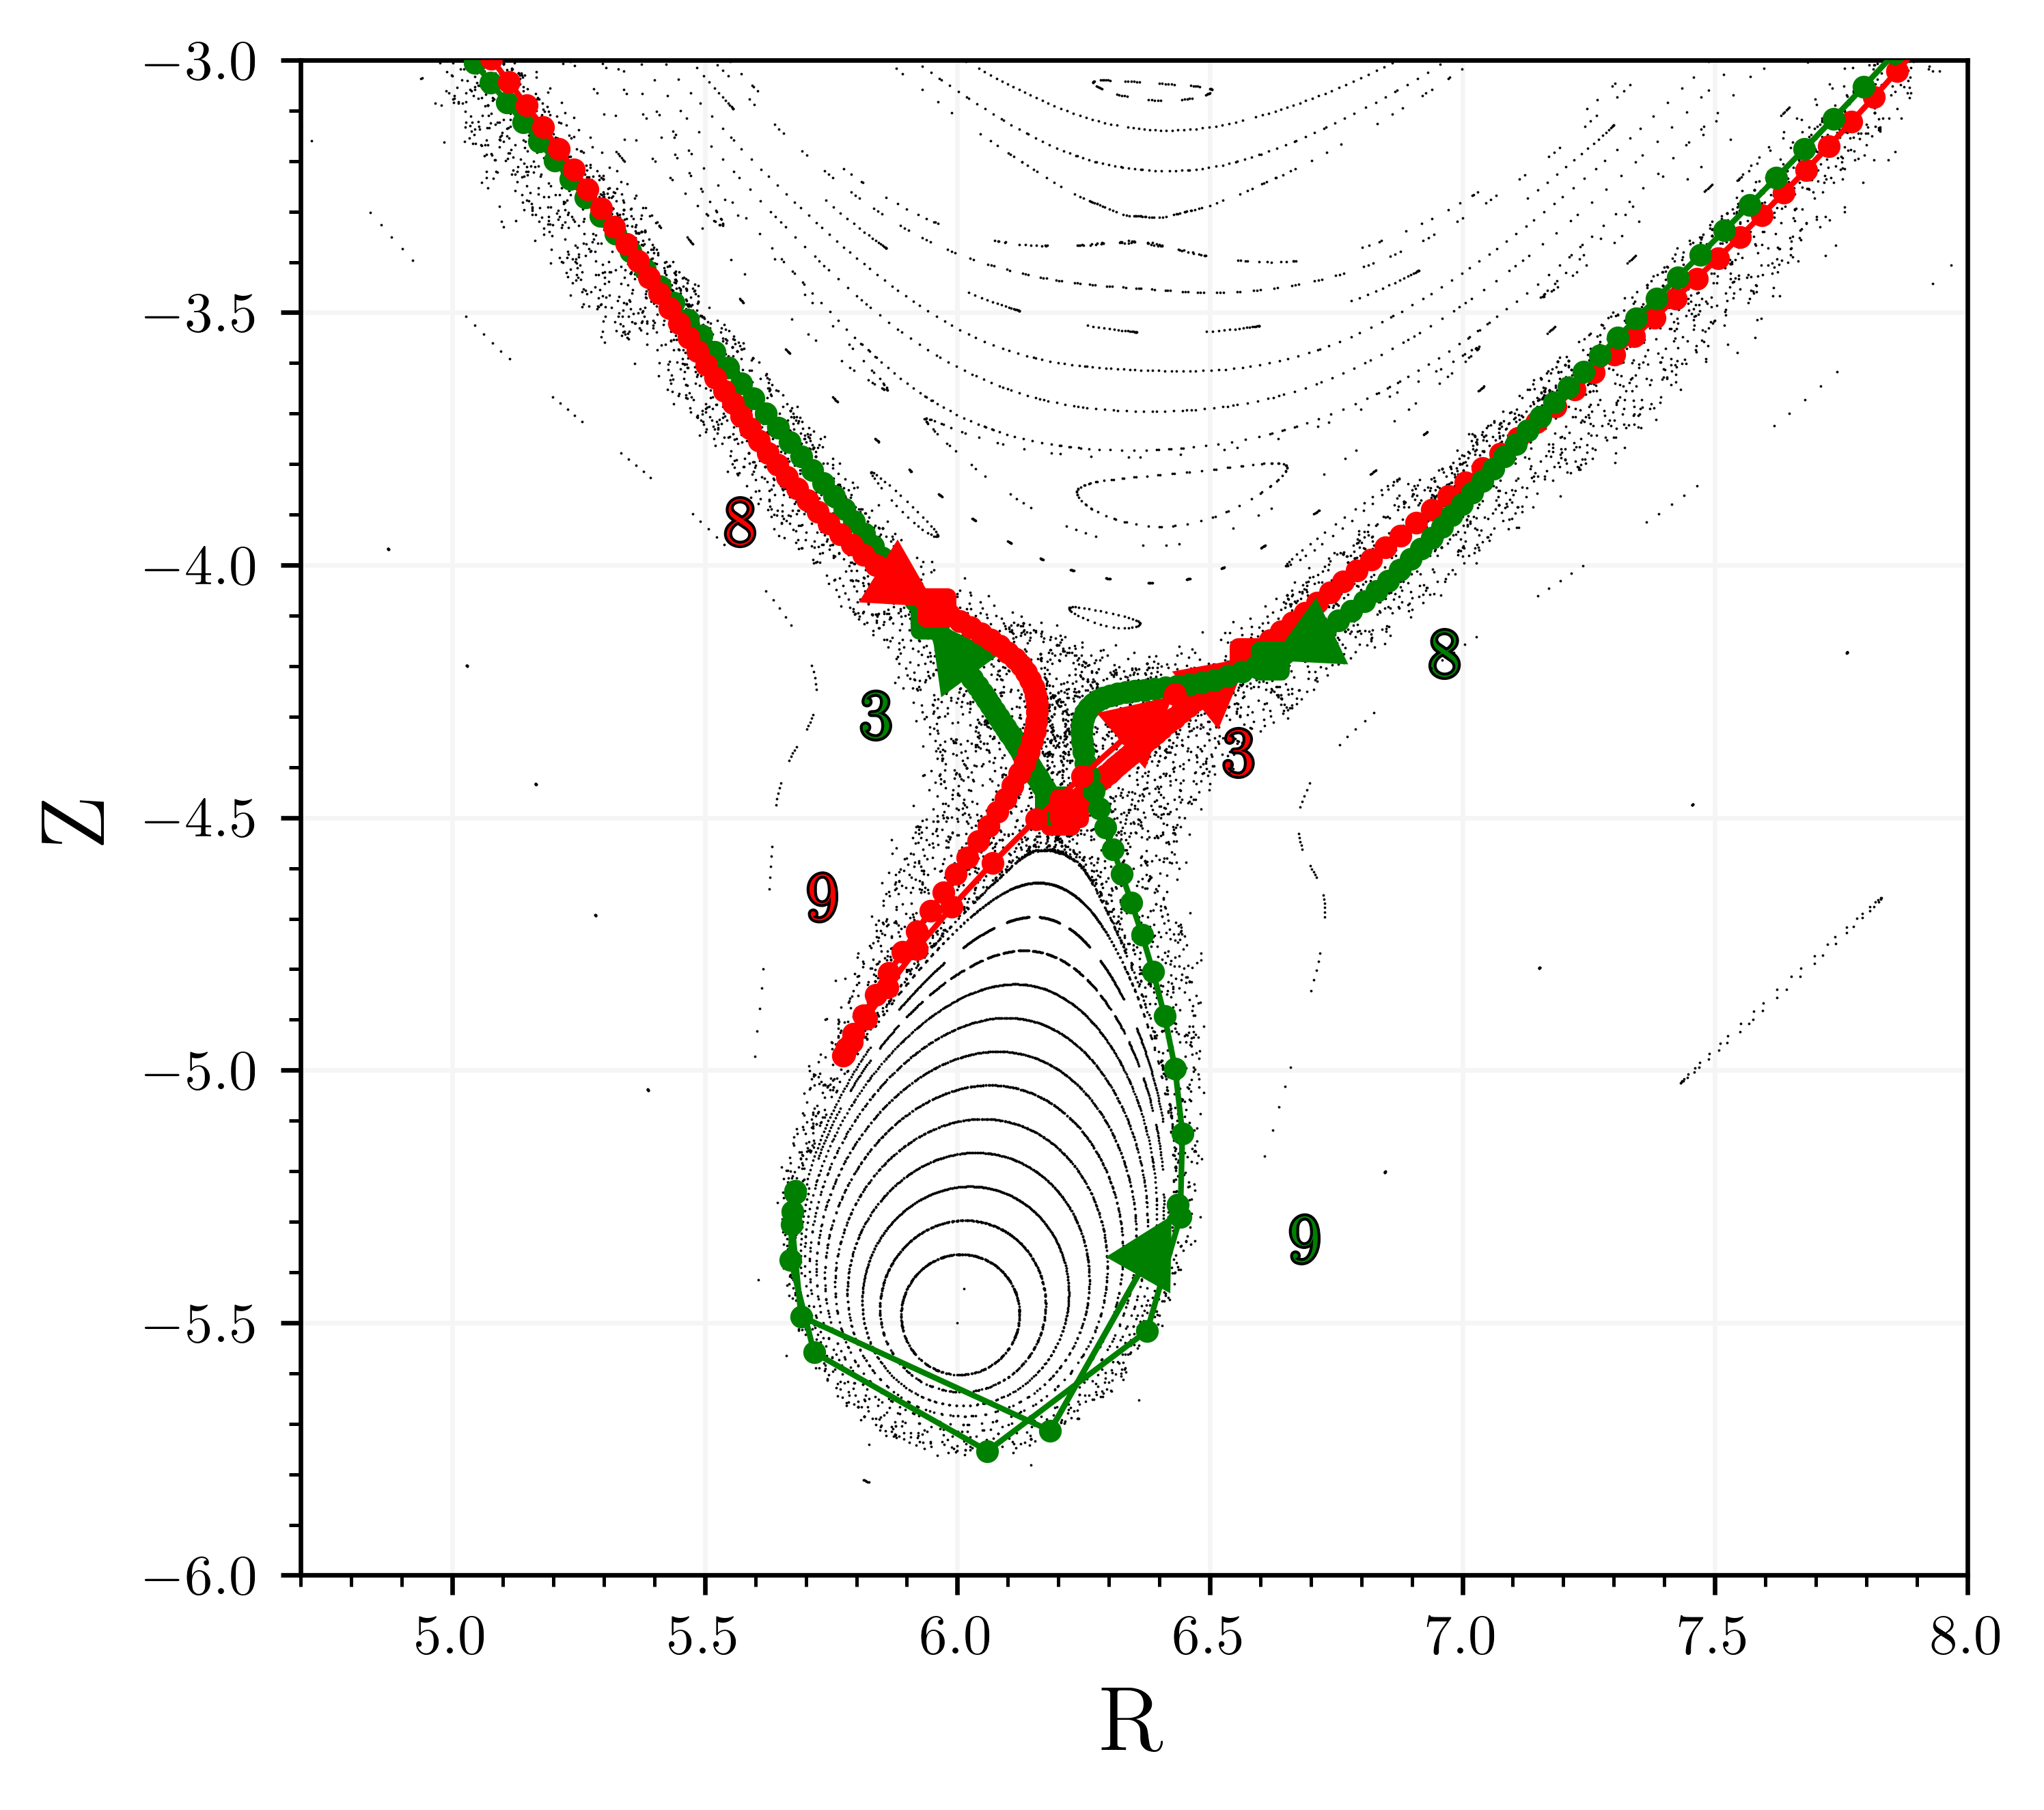
\includegraphics[width=\textwidth]{images/manifold/manifold_closer.png}
            \caption{}
            \label{fig:man-b}
        \end{subfigure}
    \end{minipage}%
    \begin{minipage}{0.5\textwidth} % Adjust width as needed
        \centering
        \begin{subfigure}[b]{\textwidth}
            \centering
            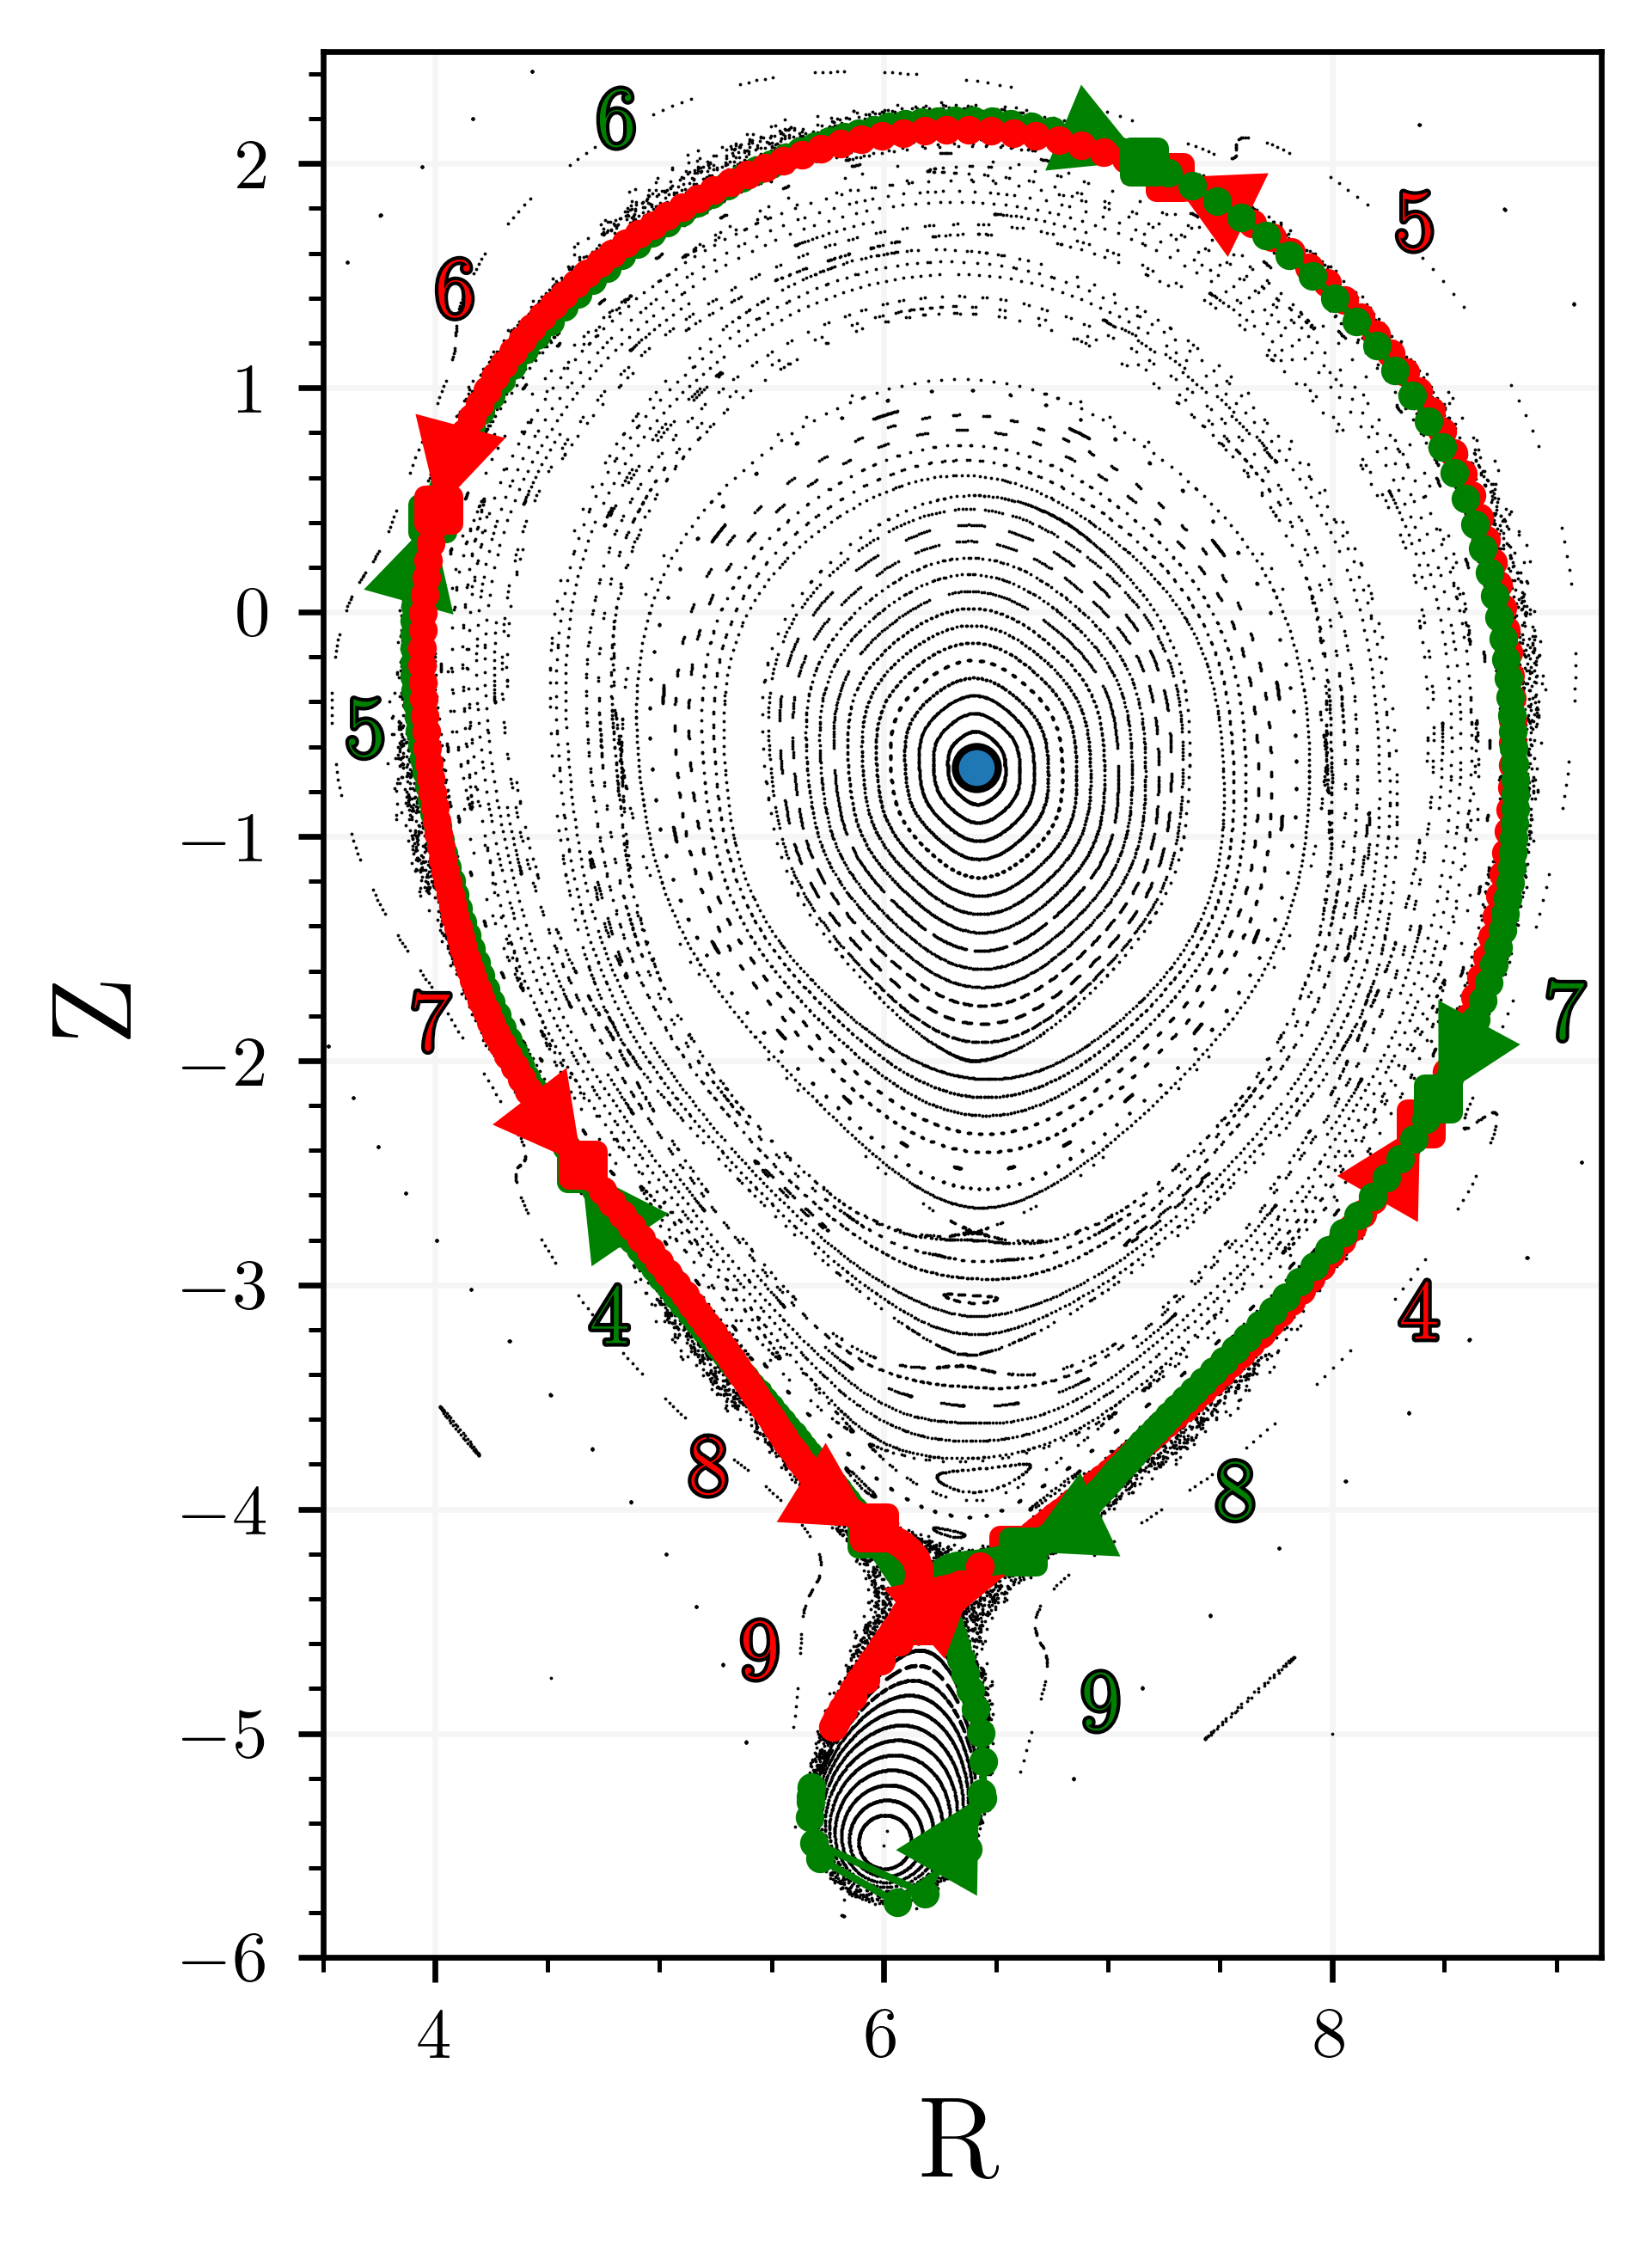
\includegraphics[width=\textwidth]{images/manifold/manifold.png}
            \caption{}
            \label{fig:man-c}
        \end{subfigure}
    \end{minipage}
    \caption{Different steps of the manifold plotting process for the perturbed Toy-Tokamak. The starting point in the linear regime is shown in (a) while (b) and (c) shows the evolution of those initial segments while applying  }
    \label{fig:manifold-algo}
\end{figure}

The algorithm, proposed in \cite{wei_invariant_2023}, used is illustrated in \figref{fig:manifold-algo}. It consists of initialising a point on each of the manifolds: $x_s \in W^s$, $x_u \in W^u$ in the linear regime and getting their initial segments $S = ]x_s,\pmap^{-1}(x_s)]_s$ and $U = ]x_u,\pmap(x_u)]_u$. Then $S$ and $U$ are discretized with $x_{i,s/u} = x^\star + \varepsilon_i\,\textbf{e}_{s,u}$, one can set the initial $\varepsilon_i$ to be equally spaced in the exponential space $e^{\lambda_s}$ and $e^{\lambda_u}$ to better capture the change in behaviour due to exponentiality. 

\figref{fig:man-a} shows how applying $\pmap$ on the starting circles, $x_{i,s}$ in green and $x_{i,u}$ in red, maps them respectively closer and further away to the point denoted by a triangle. By further mapping the $S$ and $U$ segments with the backward and forward evolution, the entire manifolds are recovered. \figref{fig:man-b} illustrates the progress as the number of iterations increases. The short length of the initial segments is observed to increase as they leave the linear regime. At a certain point they become slightly shorter, but as they approach the saddle again they get increasingly stretched out. \figref{fig:man-c} shows how they start to wrap around the separatrix coil and go back and forth as they continue to expand, hence creating the tangle.

\section{Hetero/Homo-clinic points}

The intersection of $W^s$ and $W^u$ are of particular relevance as they are points for which $\pmap^k(x)$ converges to $x_s^\star$ for $k \to \infty$ and $x_u^\star$ for $k \to -\infty$. The points $p$ in $\mathcal{H} = W^s \cap W^u / \{x^\star\}$ are called heteroclinic points if points $x_s^\star \neq x_s^\star$ and homoclinics otherwise. An immediate equivalence class for the points $p$, $q$ in $\mathcal{H}$ is given by $[p] = [q]$ if $p$ can be obtained by mapping the point $q$ for some number of forward or backward iterations. The 3d trajectory of an homo/heteroclinic in the toroidal device is linked to the 2d crossings with the relation $[p_i] = [p_j]$.

A particular type of intersection, the \textit{primary} homo/hetero-clinic points, is of interest. They are defined formally in \cite[p.14]{hohloch_homoclinic_2017} and they represent geometrically the intersections $p\in\mathcal{H}$ between the two manifold for which the curves that joins $x^\star$ to $p$ in $W^s$ and $W^u$ only intersect at their endpoint. They are formally defined in \cite[p.14]{hohloch_homoclinic_2017} and geometrically represent the intersections $p\in\mathcal{H}$ between the two manifolds for which the curves connecting $x^\star$ to $p$ in $W^s$ and $x^\star$ to $p$ in $W^u$ intersect only at their endpoints. An algorithm for finding these crosspoints is presented here, based on a suggested approach by Matt Landermann. In Sec.\ref{sec:manif}, it has been seen that after $6$ forward/backward iterations the two curves $\mathcal{P}^{-6}(S)$ and $\mathcal{P}^{6}(U)$, images of the initial segments, are intersecting. Writing $x_{0,s}$ and $x_{0,u}$ two starting points in $S$ and $U$, the goal is to find the root of~:
\begin{equation*}
    \mathcal{P}^{-6}(x_{0,s}) - \mathcal{P}^{6}(x_{0,u})
\end{equation*}
which can be achieved by an optimization process\footnote{Using for instance scipy root}. In a more general context, if $S$ and $U$ cross after $j$ iteration on $S$ and $k$ iteration on $U$, then every $(n_s, n_u)$ pair such that their sum equals $j+k$ will also work and the hetero/homoclinics can be searched in a region closer to the fixed point, where the shape of one of the manifolds is a bit more twisted, making the algorithm converge better. \figref{fig:clinic-search-a} shows the initial step for the primary homoclinic search in the perturbed Toy-Tokamak with $n_s = 8$ and $n_u = 4$. The optimisation tries to find starting points such that the length of the black arrow is zero.
\begin{figure}[h!]
    \centering
    \begin{subfigure}[c]{0.41\textwidth}
        \centering
        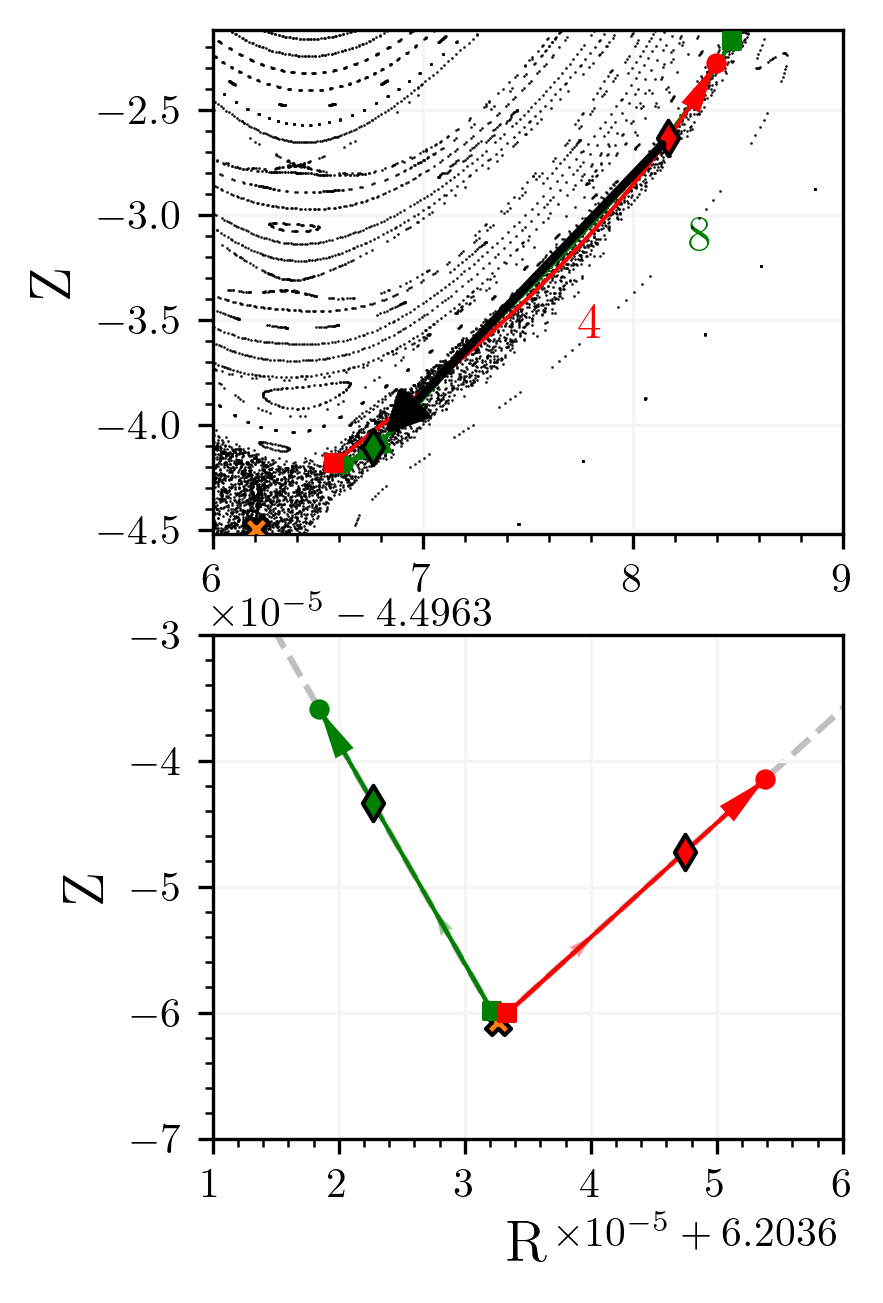
\includegraphics[width=\textwidth]{images/clinicsearch/clinic_start.png}
        \caption{}
        \label{fig:clinic-search-a}
    \end{subfigure}
    \hfill
    \begin{subfigure}[c]{0.58\textwidth}
        \centering
        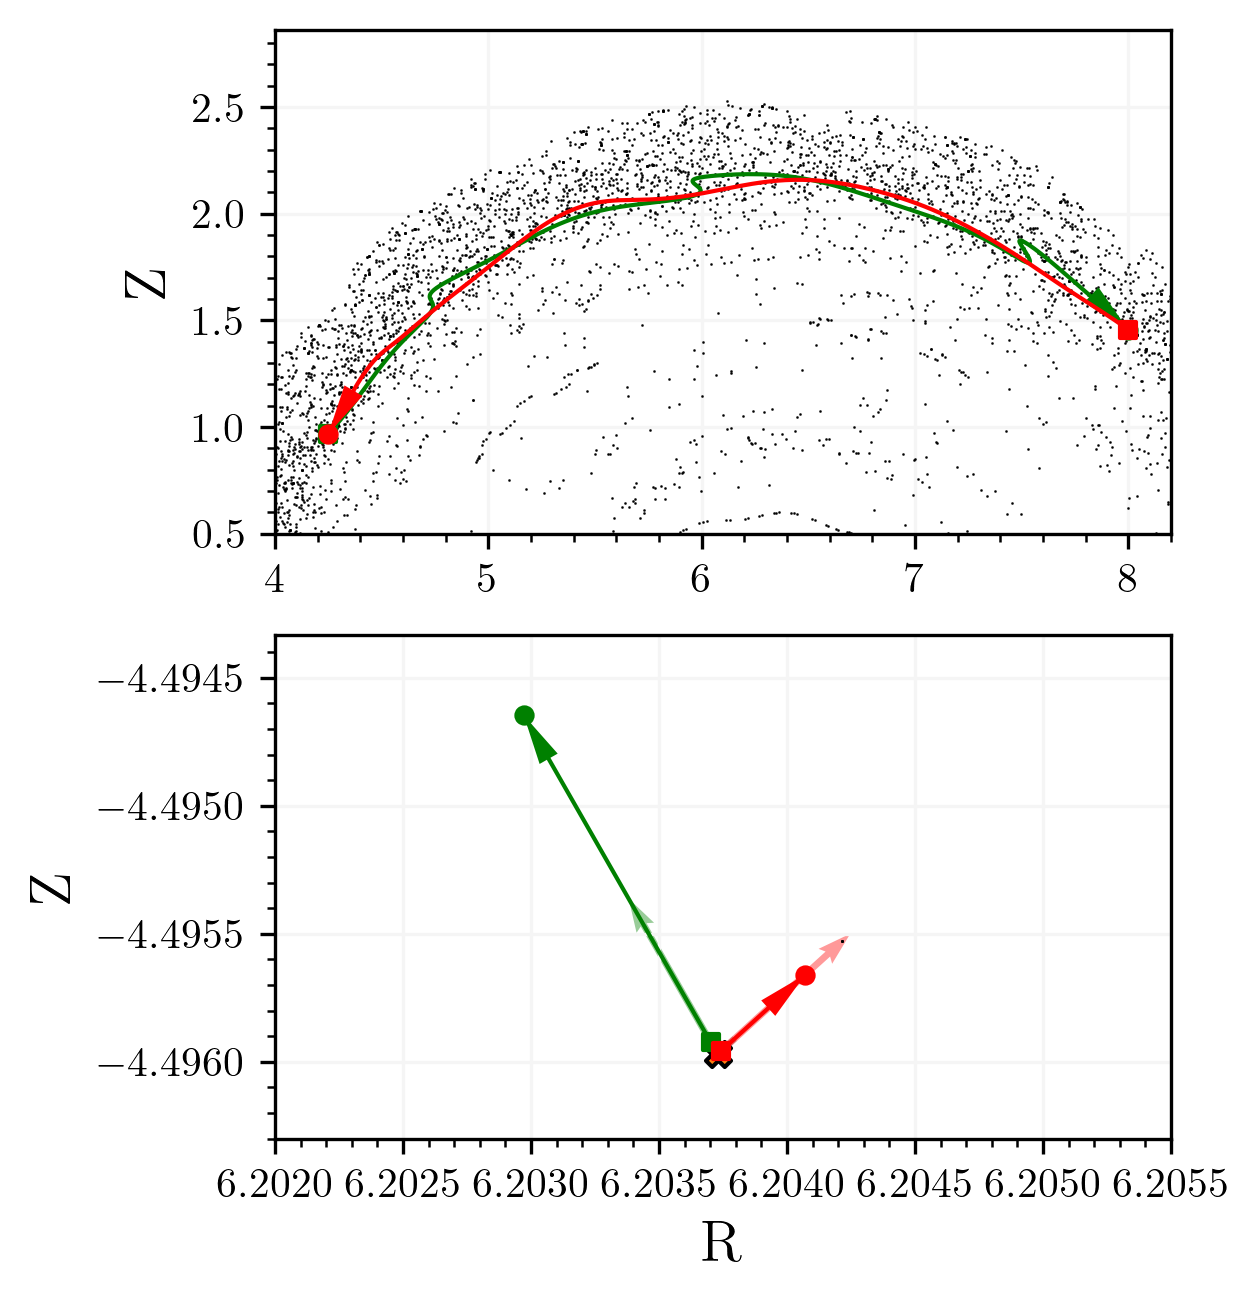
\includegraphics[width=\textwidth]{images/clinicsearch/search_domain.png}
        \caption{}
        \label{fig:clinic-search-b}
    \end{subfigure}
    \caption{homoclinic points seach. (a) initial search guess mapped $n_s = 8$ and $n_u = 4$ times. (b) same path idea showing the initial segments for the where there is more than two homolcinics to search for.}
    \label{fig:clinic-search}
\end{figure}

This works well to find a first homoclinic point. However there are at least another primary homoclinics to find in the intersection. 

By resetting the initial segment to take the homoclinic as their starting point will show how many other primary intersection are yet to be found. 

\figref{fig:clinic-search-b} shows this new 

segments with the same toybox but with a perturbation $m/n = 18/3$. We see that there are 6 primary crossings in total and in the 12/2 case has 4 primary homoclinics. It seems that the relation is simply the mode $n$ however some other perturbation did not follow that and due to the mixed mode perturbation it is hard to conclude something. maybe there is a clever way to relate  the mode perturbation and related to the mathematics of prime number. This an interesting subject to further consider.

Here a clever search of the two curve may exist. However using the same idea as for the first, minimizing this time $\mathcal{P}^{-n_s-1}(x^s) - \mathcal{P}^{n_u}(x^u)$, but using a starting point of the form     
\begin{align*}
       x^s = x^\star+\lambda_s^{i/n_h}\varepsilon_s^1 \textbf{e}_s \quad
x^u = x^\star+\lambda_u^{i/n_h}\varepsilon_u^1 \textbf{e}_u \quad\text{with}\quad i = 1,...,n_h
\end{align*}
will in most cases converge to the right homoclinic. This works because due to the taylor expansion the starting epsilon will be mapped to $\lambda_{s,u}\varepsilon$ and thus after $\lambda_{s,u}^{n/n}$ one recovers the first point while having $n_h$ intersections. Note that in general this optimization is not a easy task as the structure of the distance function looks like a rosenbruck optimization, were a valley is present when the two manifold are travelled in opposite directions. A robust understanding/way to know the number of primary homoclinics and algorithm to find them is welcome but, i think, yet to be thought of at least for the problem described here.

\section{Turnstile}

In the non chaotic case of the tokamak, the separatrix defines the boundary of the confined region and is also called the Last Closed Flux Surface. 

When chaos is present, on can still define an interior region by setting as boundary the segment $[x_s^\star,p]\cup[p,x_u^\star]$
and $[x_s^\star,q]\cup[q,x_u^\star]$ for p and q primary heteroclinic in the manifold that were the unbroken separatrix. This region is where the remaining closed field line of a tokamak are and where the island will be in general. Meiss calls it the resonance zone \cite{meiss_thirty_2015}, and looks a the well studied chirikov standard ap on the cylinder ~:
\begin{align*}
   p_{n+1} &= p_{n} -\frac{K}{2\pi}\sin(2\pi\theta_n)\\
   \theta_{n+1} &\equiv \theta_{n} + p_{n+1} \pmod{1} 
\end{align*}
The map is area preserving and its usufull because there is the k parameter that plays the role of a perturbation and brings in more chaos as it increases. Particularly, Meiss looks at the $(0,1)$ orbit when $K=1.5$. \figref{fig:standardmap-turn} shows the resonance region for this orbit and highlights the stable and unstable manfiolds. $w^s$ and $W^u$ define also boundary of lobe, taking one of the lobe and we see that it will be map to a next lobe. This is such that there will a time when the lobe is mapped out or in of the resonance zone. Due to the area preservation property we can say that the exiting set, $E$ such that the point go out applying the map, and the entry set $I$ for point outside of the resonance map in, have the same area. The area of the lobes are indicative of the degree of chaos because we know that if we compare it with the island total area it represents the relative amount of the island being subject to the chaos, while the rest are closed surfaces. Meiss shows how to calculate this indicative area in a general map which conserved an exact volume form $\Omega$ which is the $\Omega = d\alpha$ and finally uses a propriety of the exactness of the map, if the map is volume preserving and exact then he puts the general equality~:
\begin{equation}
    \mu(R) = \int_R \Omega = \int_{\partial R} d\alpha =  \int_{\mathcal{U}} \alpha - \int_{\mathcal{S}} \alpha = 
\end{equation}
This obscure mathematical formulation can be explain for the standard map as follow : as $1 = \nabla\times (x\,\textbf{e}_y)$ we can use stokes theorem to write~:
\begin{equation}
    \mu(R) = \int_R 1 = \int_{\partial R} \nabla\times (x\,\textbf{e}_y) =  \int_{\mathcal{U}} x\,\textbf{e}_y\cdot\textbf{dl} - \int_{\mathcal{S}} x\,\textbf{e}_y\cdot\textbf{dl}.
\end{equation}
In the case of a the last part says that summing on the lagrangian function as the time goes to infinty and minum infinity. 

\begin{figure}[H]
    \centering
    \begin{subfigure}[t]{0.49\textwidth}
        \centering
        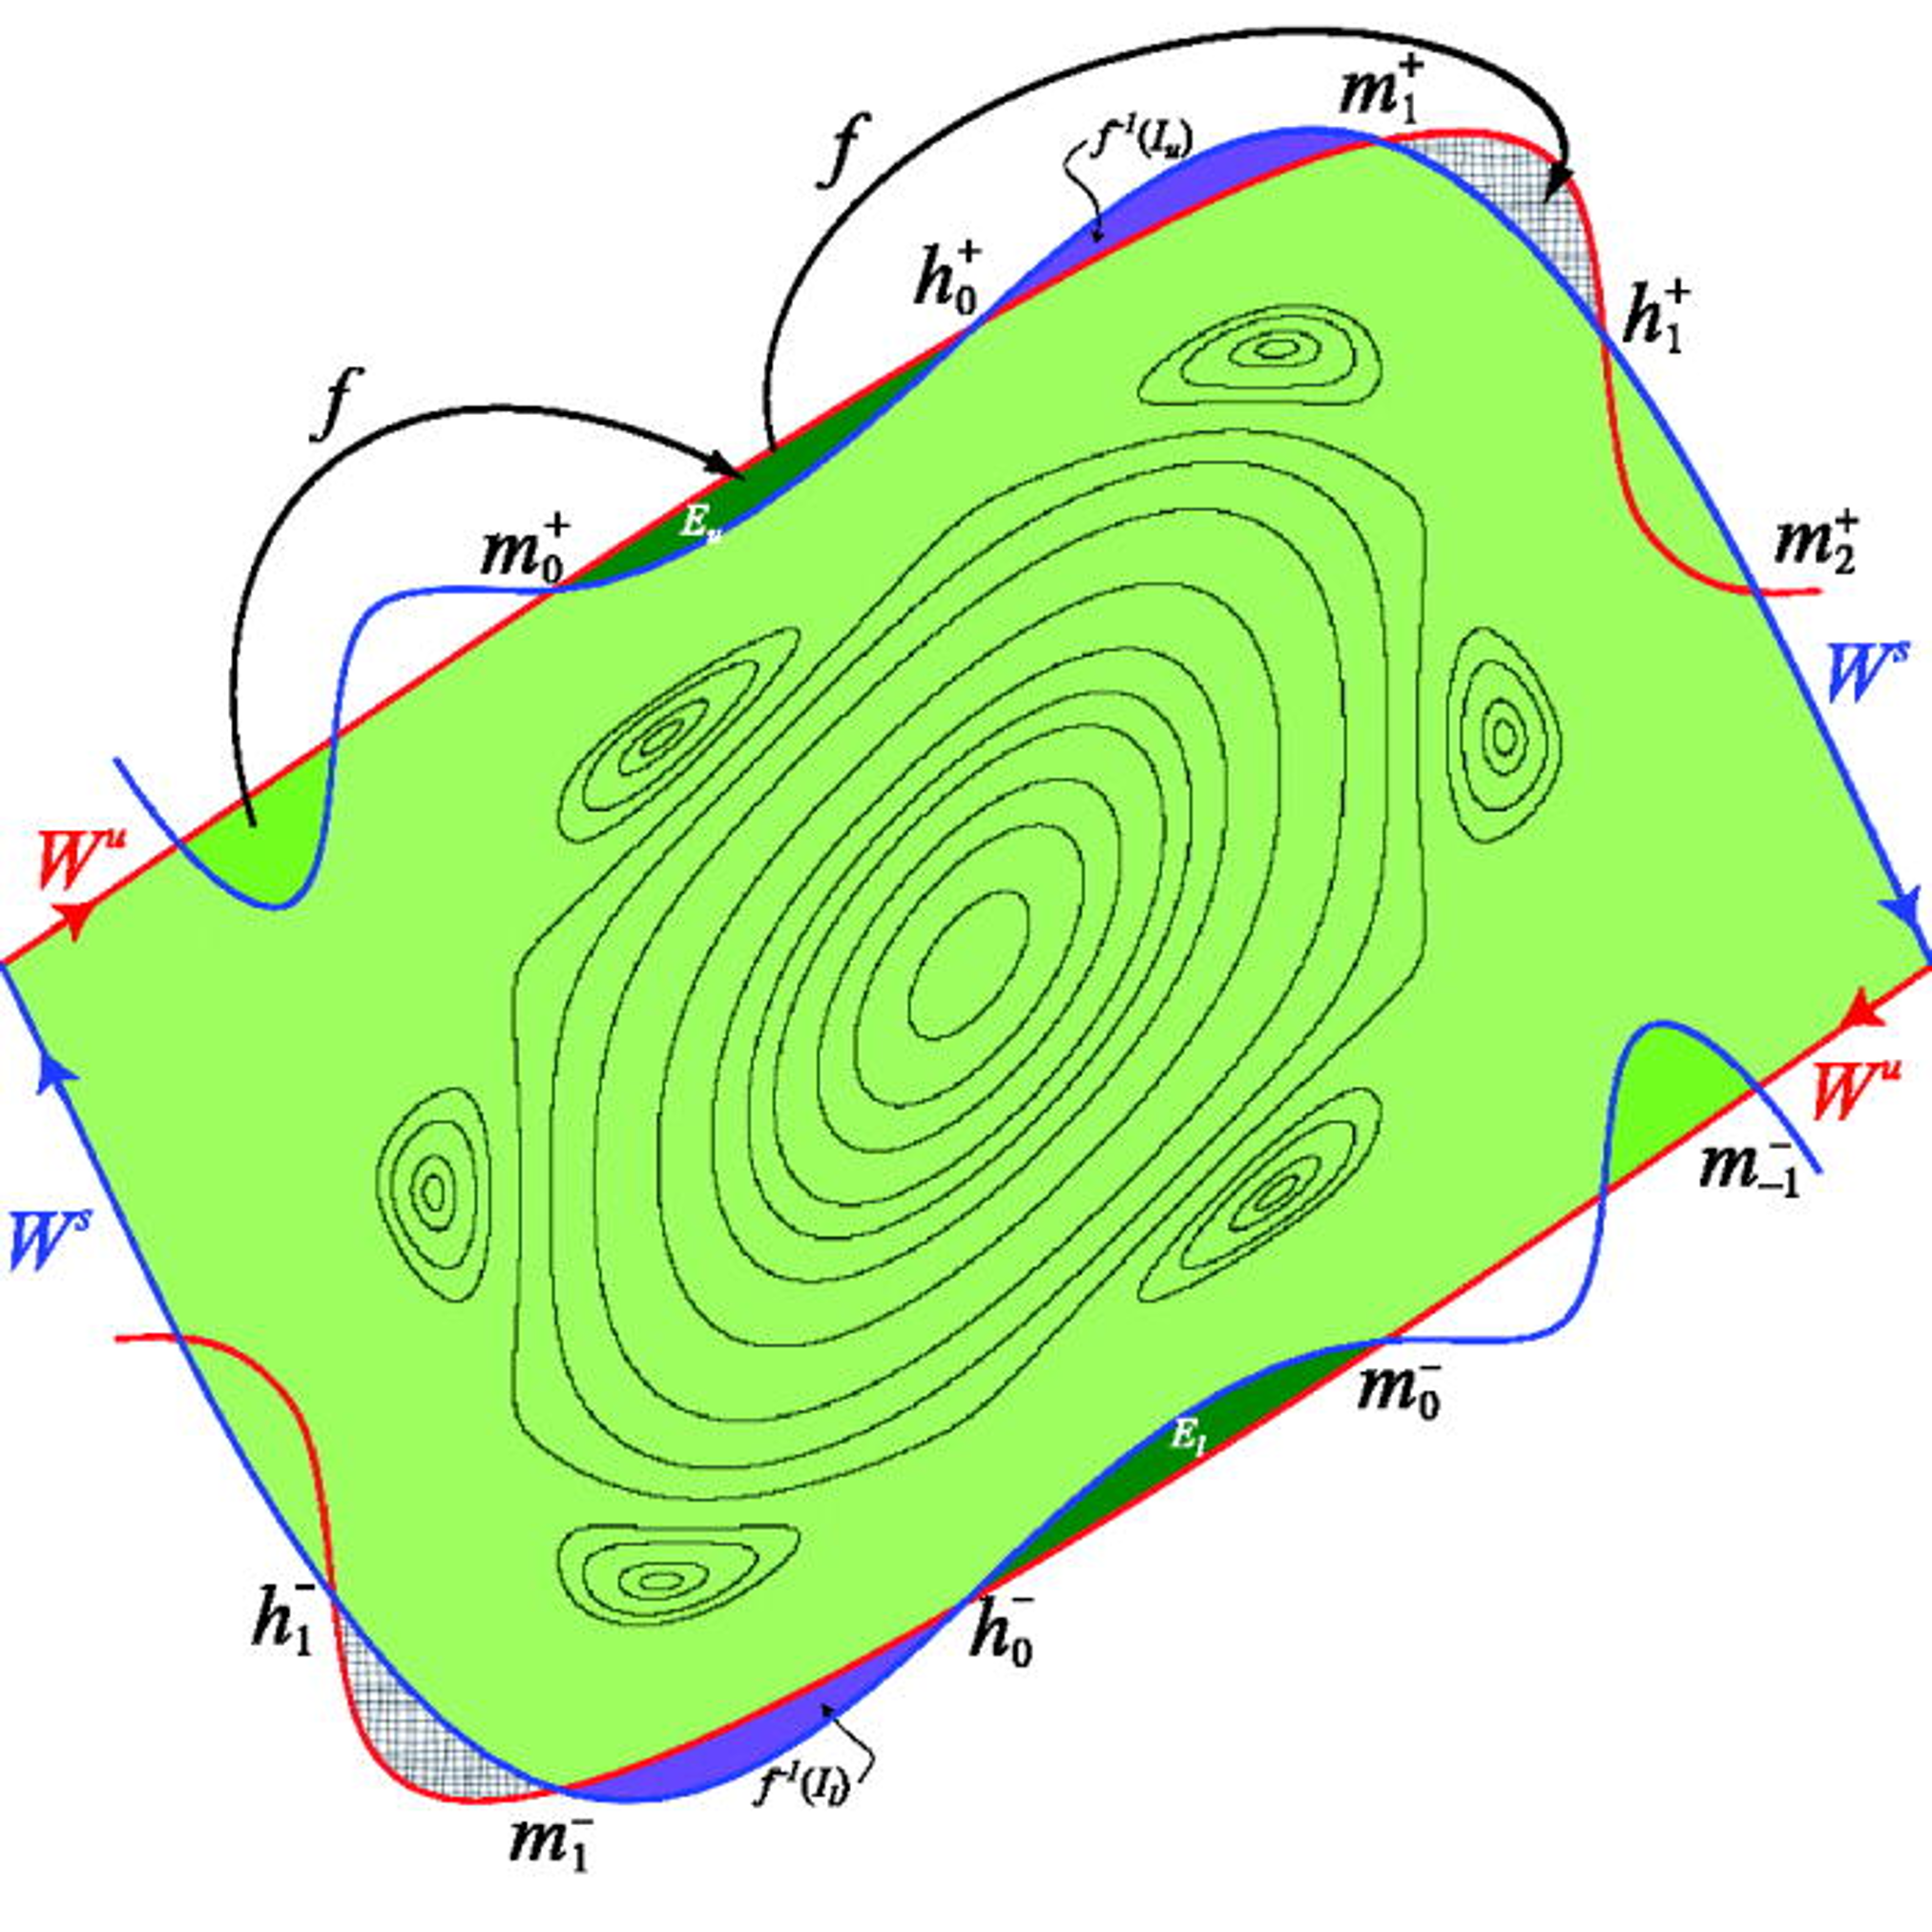
\includegraphics[width=\textwidth]{images/turnstile/01Resonance.png}
        \caption{}
        \label{fig:standardmap-turn}
    \end{subfigure}
    \hfill
    \begin{subfigure}[t]{0.49\textwidth}
        \centering
        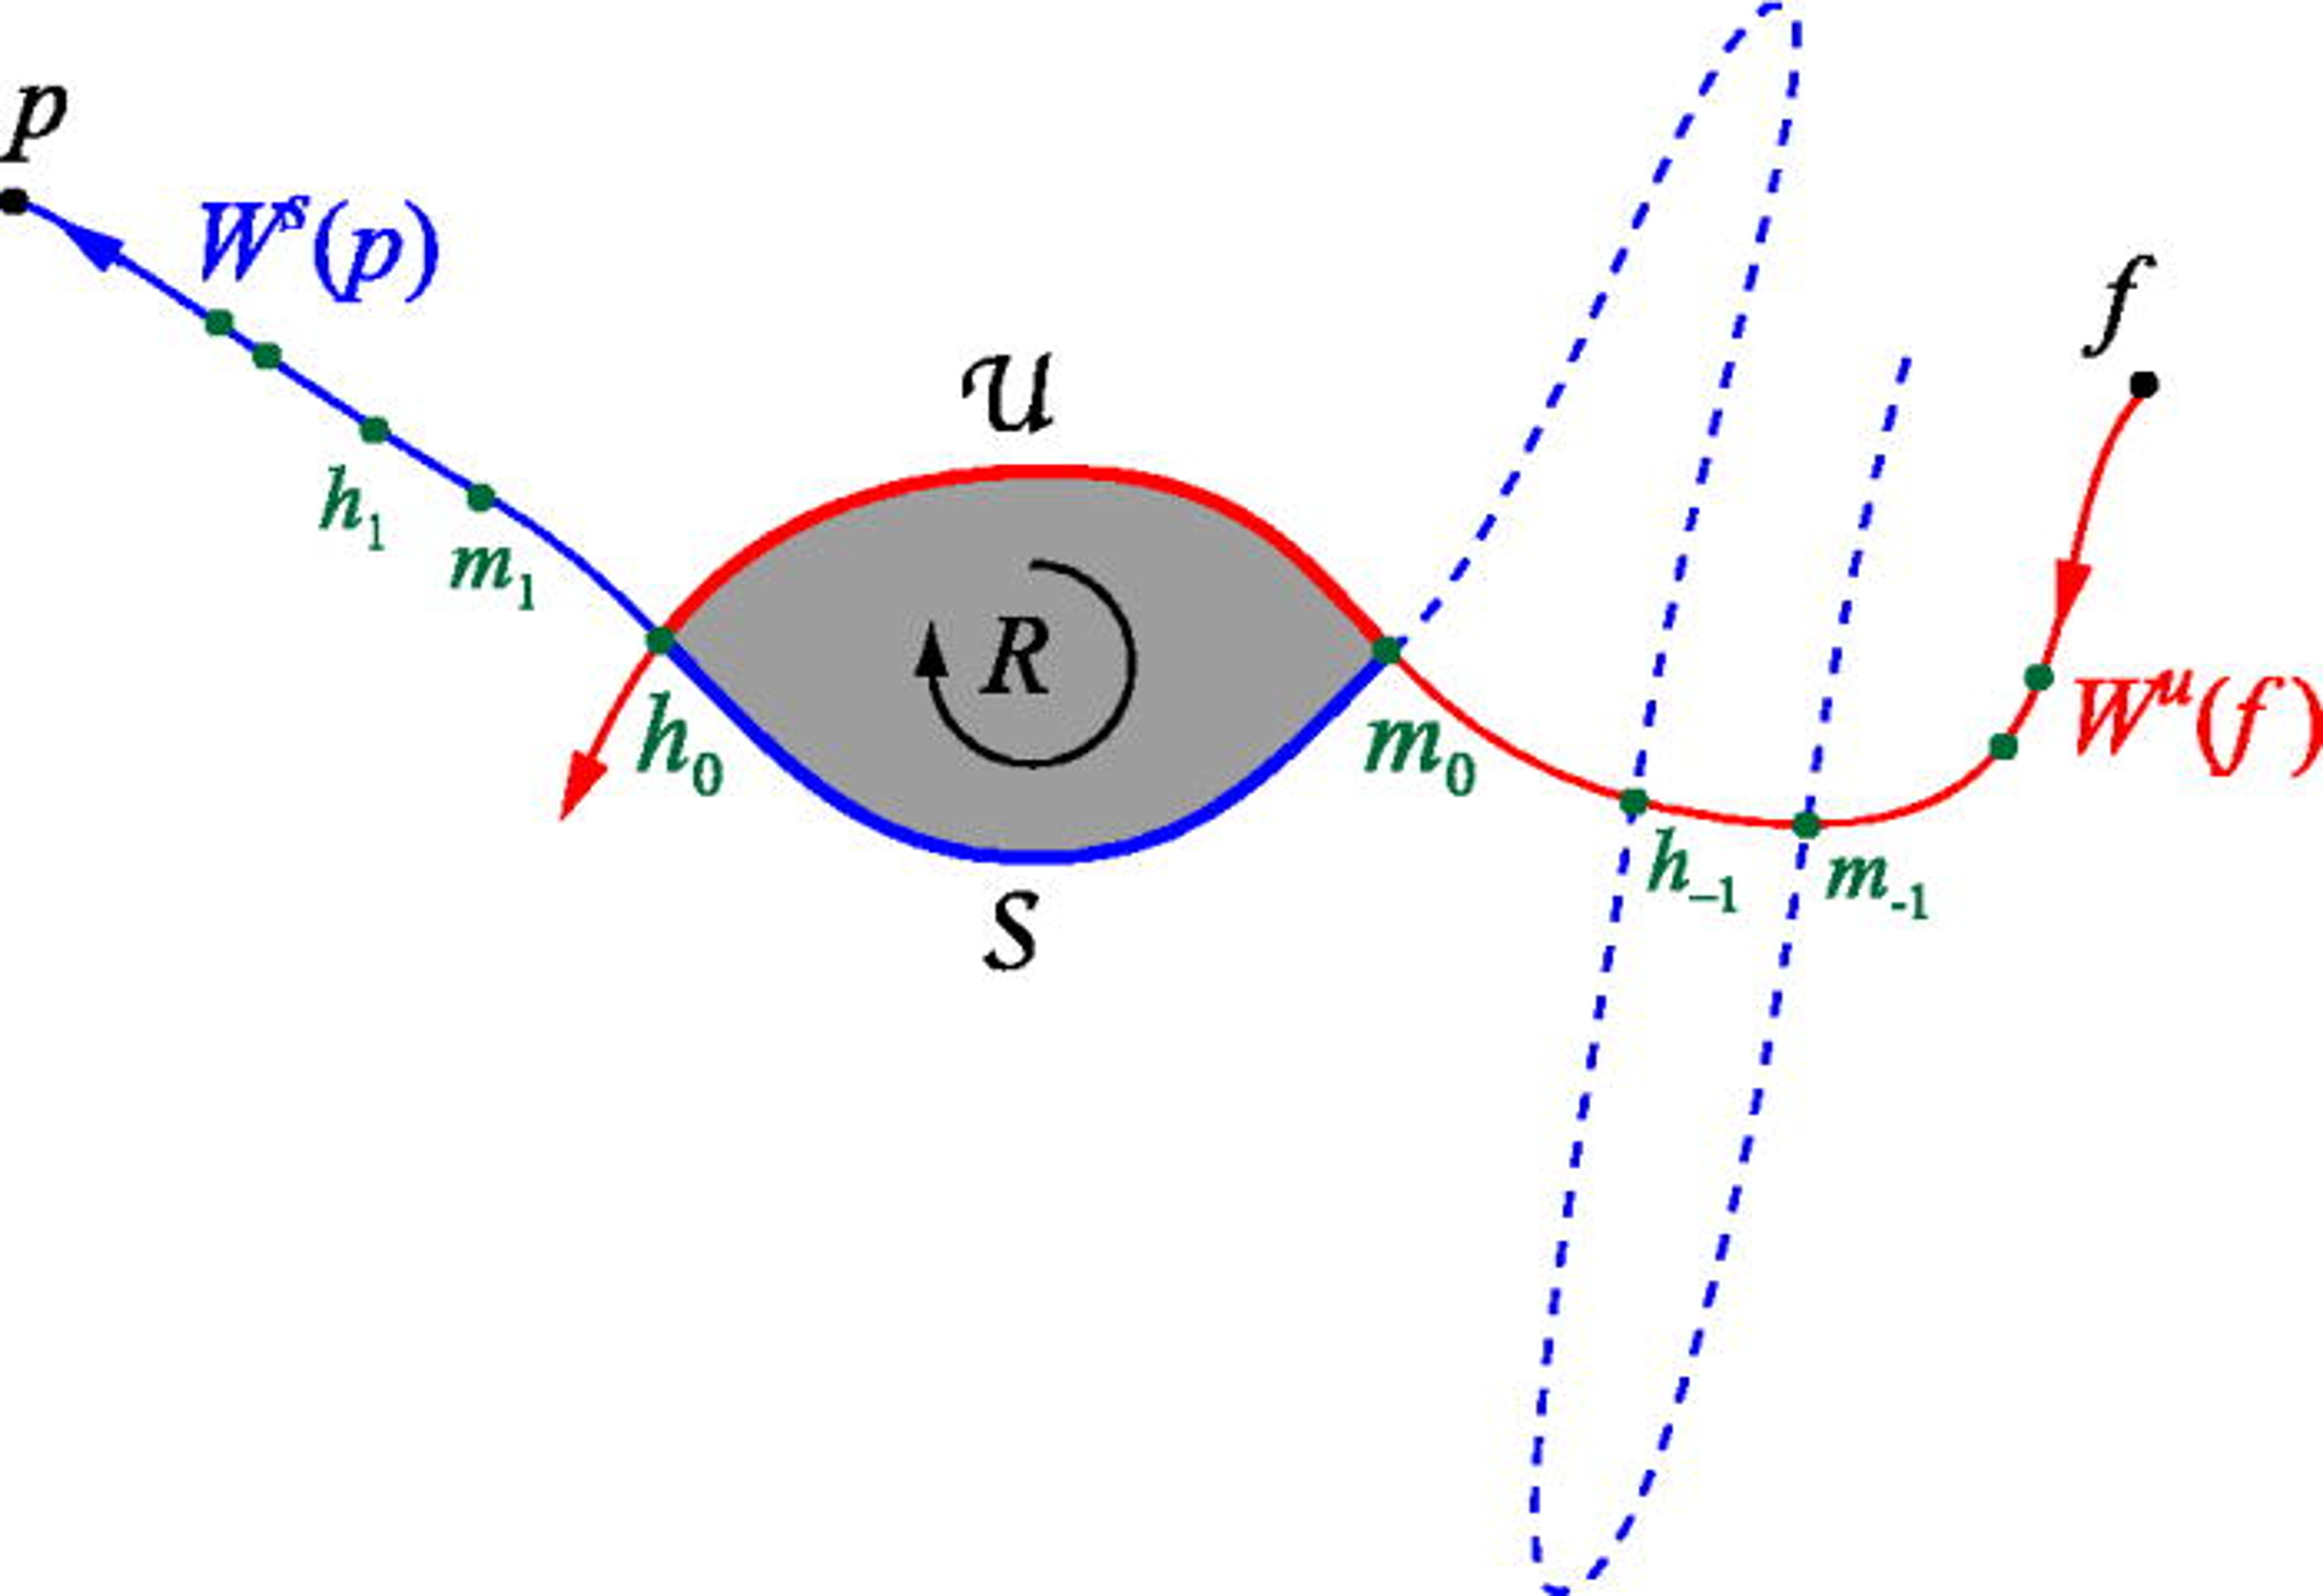
\includegraphics[width=\textwidth]{images/turnstile/2DLobe.png}
        \caption{}
        \label{fig:meiss-countour}
    \end{subfigure}
    \caption{Schematic representation of a turnstile in (a) for the resonance zone of the (0,1)-orbit of the standard map with $K = 1.5$, (b) for the tangle structure formed by the manifolds $W^s(p)$ and $W^u(f)$ of two $f$ and $p$ saddles. In both cases the orbit intersections of primary homo/heteroclinics are denoted by $h_i$ and $m_i$. The figures are taken from \cite{meiss_thirty_2015}.}
\end{figure}

\subsection{Adapting Meiss's action principle for the map $\pmap$}
\newcommand{\Sl}{\Sigma_{lobe}}
\newcommand{\Se}{\Sigma_{ev}}

There is a nice analogy with the conservation of the flux and the fact that $B$ equals ($\nabla\times\textbf{A}$), more precisely the mathematical description of the maxwell equations using differential forms. In the case of the $\pmap$, then we a priori don't now that there is only one lobe for the turnstile, we do know that for the total sum $\mu(E) = mu(I)$. The calculation of the flux through one lobe is still then the most general.

\begin{figure}[H]
    \centering
    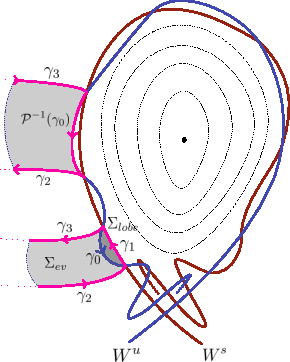
\includegraphics[width=0.5\textwidth]{images/turnstile/tokamak-tangles.png}
    \caption{Schematic representation of the calculation of the turnstile area in a homoclinic tangle. The tangle is formed by $W^s$ and $W^u$ in a chaotic configuration of the Toy-Tokamak with perturbation $m/n = 6/1$. A turnstile lobe is depicted as $\Sl$ with boundary $\gamma_0 + \gamma_1$ and the boundary of a more complex surface with identical flux $\Sigma = \Sl + \Se$ is especially emphasised in pink.}
    \label{fig:tangle-3d}
\end{figure}

The boundary $\partial\Sl$ of a specific lobe $\Sl$ of the turnstile can be subdivided, as illustrated in \figref{fig:tangle-3d}, into two curves : $\gamma_0\subset W^u$ and $\gamma_1\subset W^s$. $\gamma_0$ joins the intersections $h_0$ of the homoclinic $h$ field line to the intersection $m_0$ for the second homoclinic $m$ and $\gamma_1$ returns from $m_0$ to $h_0$. Using Stokes theorem, the flux  $\Phi_{lobe}$  through $\Sl$ can therefore be written as~:
\begin{equation}\label{eq:contour-1}
    \Phi_{lobe} = \int_{\Sl} \textbf{B}\cdot\textbf{dS} = \int_{\Sl} \nabla\times\textbf{A}\cdot\textbf{dS} = \int_{\gamma_0+\gamma_1} \textbf{A}\cdot \textbf{dl}.
\end{equation}
To directly, numerically, calculate the integral in \equref{eq:contour-1} requires the curves $\gamma_0$ and $\gamma_1$ to be discretized. In practise, it would mean that many initial positions need to be set in the linear regime of $W^u$ and $W^s$ in between position of $h$ and $m$, then their field line have to be traced up until they form the boundary $\partial\Sl$. The number of points must be sufficient and appropriately tuned to describe the bending of the manifolds well enough to avoid introducing too many errors. Although it is not necessary to locate the homoclinics beforehand, and further approximations (such as assuming that the points describe a Bezier curve) are possible improvements to such a method, it becomes very expensive to increase the accuracy as it means more integrations have to be performed. This will prove impractical in a general stellarator field. A more elegant algorithm for calculating the lobe flux is suggested, based on the principle of the turnstile calculation for the standard map presented by Meiss [REF].

Tracing the curve $\gamma_0$ backward around the torus generates a surface $\Se$, depicted in \figref{fig:tangle-3d}, for which the normal $\textbf{dS}$ is always orthogonal to the magnetic field $\textbf{B}$ according to definition of FLT. It means that the flux through $\Sigma \coloneqq \Sl+\Se$ is equal to the one through $\Sl$ and \equref{eq:contour-1} becomes~:
\begin{equation}\label{eq:contour-2}
    \Phi_{lobe} =  \int_{\Sl} \textbf{B}\cdot\textbf{dS} = \int_{\Sl+\Se} \textbf{B}\cdot\textbf{dS} = \int_{\partial\Sigma} \textbf{A}\cdot \textbf{dl}.
\end{equation}
The oriented boundary $\partial\Sigma = \gamma_1 + \gamma_2 + \gamma_3 + \gamma_4$ is composed of four paths~: $-\gamma_2$ and $\gamma_4$ are obtained as the trajectories of the homoclinics $h$ and $m$ from $h_{-1}\coloneqq\pmap^{-1}(h_0)$ and $m_{-1}\coloneqq\pmap^{-1}(m_0)$ to $h_{0}, m_{0}$ around the torus. $\gamma_1$ and $\gamma_3$ which will be referred to as joining curves and lie in the Poincare section. As for $\gamma_0$, $\gamma_3$ is part of the unstable manifold and while $\gamma_0$ connects $h_0$ to $m_0$, $\gamma_3$ joins $h_{-1}$ to $m_{-1}$. A flat representation of the tangle structure is shown in \figref{fig:flat-tangle}. The unstable manifold, initially straight around the fixed point $x_u^\star$, has an increasing curvature as it approaches $x_s^\star$. The stable manifold shows a similar behaviour with the points reversed. Their intersections $h_i$ and $m_i$ are shown as a circle and a square respectively, and the joining integral path can be seen more clearly.

\begin{figure}[H]
    \centering
    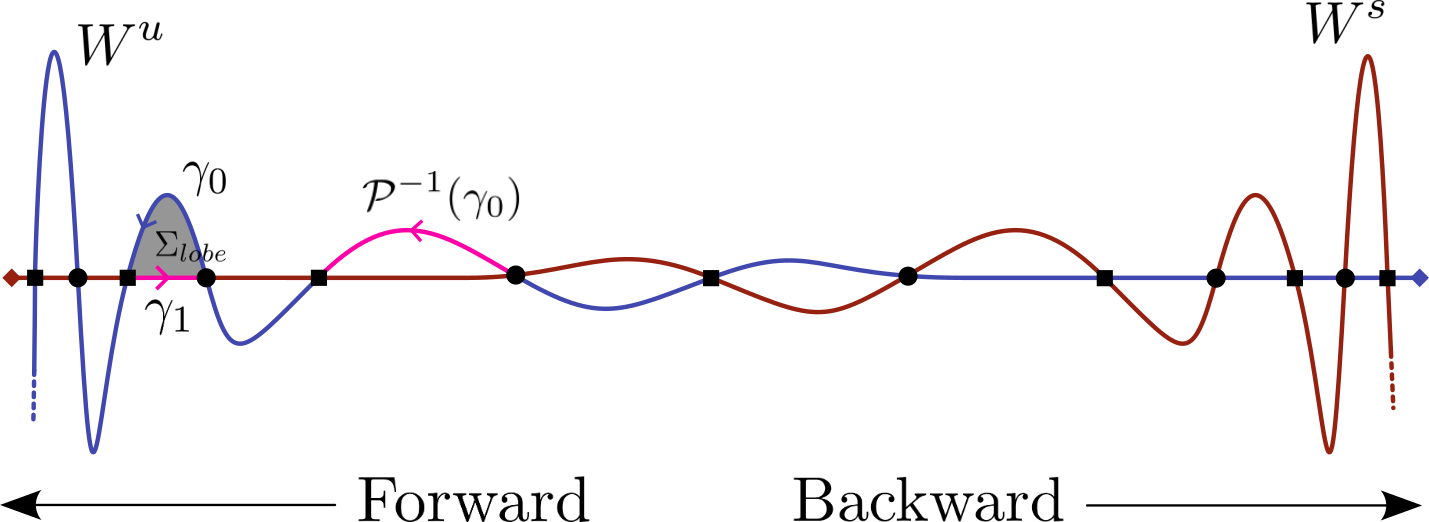
\includegraphics[width=0.8\textwidth]{images/turnstile/line_tangle.png}
    \vspace{10px}
    \caption{Flatten out version of the manifold tangle structure between two saddle fixed points $x_s^\star$ and $x_u^\star$. The forward evolution $\pmap$ maps points close to $x_u^\star$ in the direction of $x_s^\star$ and the backward evolution the opposite. Two different hetero/homo-clinics are present and are denoted by the squared and circular markers. The surface of the lobe $\Sl$, as well as the joining curves $\gamma_1$ and $\gamma_3$ are highlighted.}
    \label{fig:flat-tangle}
\end{figure}

With respect to the integration path taken in \equref{eq:contour-1}, the path of $\eqref{eq:contour-2}$ contains the trajectory of the homoclinic as part of the contour. The relationship with the formula given by Meiss appears, however, the difficulty of finding $\gamma_1$ and $\gamma_3$ remains. 

To take care of those joining integrals, note that the argument for $\Se$ is still true by applying the map more than once backward on $\gamma_0$. Indeed, by repetitively applying the backward evolution, $\pmap^{-k}(\gamma_0)\subset W^u$ joins $h_{-k}$ and $m_{-k}$ that are closer and closer as they approach $x_u^\star$. The length of the the curve converges to 0 as $t\to\infty$ and using Cauchy-Schwartz inequality, the integral of $\textbf{A}\cdot\textbf{dl}$ also converges to zero~:
\begin{equation*}
    \int\limits_{\pmap^{-k}(\gamma_0)} \textbf{A}\cdot\textbf{dl} \leq \int\limits_{\pmap^{-k}(\gamma_0)} \Vert\textbf{A}\Vert \Vert\textbf{dl}\Vert \leq\, L(\pmap^{-k}(\gamma_0))\max\limits_{\textbf{x} \in\pmap^{-k}(\gamma_0)}\Vert\textbf{A(\textbf{x})}\Vert \lesssim L(\pmap^{-k}(\gamma_0)).
\end{equation*}
Following the trajectory of the homoclinic points $h_0$ and $m_0$ until they converge to the fixed point, the length of $\gamma_1$ reduces to zero and it's contribution to the integral also converges to zero. Since the flux through $\Sl$ and $\pmap^k(\Sl)$ is equal (again, flux conservation of $\pmap$), the same idea as for $\gamma_3$ can be applied to $\gamma_1$. Applying the map repetitively will make the length of $\pmap^k(\gamma_1)$ and thus its contribution to the flux calculation tend to zero. Including these considerations in \equref{eq:contour-2} and taking the the number of forward and backward iterations to infinity gives~:
\begin{equation}\label{eq:flux-algorithm}
    \Phi_{lobe} = \lim\limits_{k\to\infty}\,\,\int\limits_{m_{-k}}^{m_{k}}\textbf{A}\cdot\textbf{dl} - \int\limits_{h_{-k}}^{h_{k}}\textbf{A}\cdot\textbf{dl}
\end{equation}
where the similarity with the equation provided for the standard map \cite[Eq. 21]{meiss_thirty_2015} is now striking.

The calculation of \equref{eq:flux-algorithm} requires enough iterations for the distance between the homoclinics to converges to 0. However, due to the exponential behaviour around the X-points and the inherent lack of infinity in double precision, once the field line is close to the fixed point, only a small number of crossings will be recorded before the numerical error causes the point shifted away, ending the possibility of convergence. To overcome this, and in fact to make the algorithm much more robust, a small tweak is introduced. In \equref{eq:contour-1} the difficulty of a numerical computation would have been to get the shape of the manifold precisely. Here instead for a certain finite value of $k$ : $\pmap^k(\gamma_2)$ and $\pmap^{-k}(\gamma_0)$ are mapped back into the linear regime of $x_s^\star$ and $x_u^\star$. There, the manifolds are simply segments and the joining integrals can be approximated by the midpoint rule, which requires only few evaluations of the vector potential $\textbf{A}$, but no additional field line tracing.

\begin{figure}[H]
    \centering
    \begin{minipage}[c]{0.55\textwidth} % Adjust width as needed
        \centering
        \begin{subfigure}[b]{\textwidth}
            \centering
            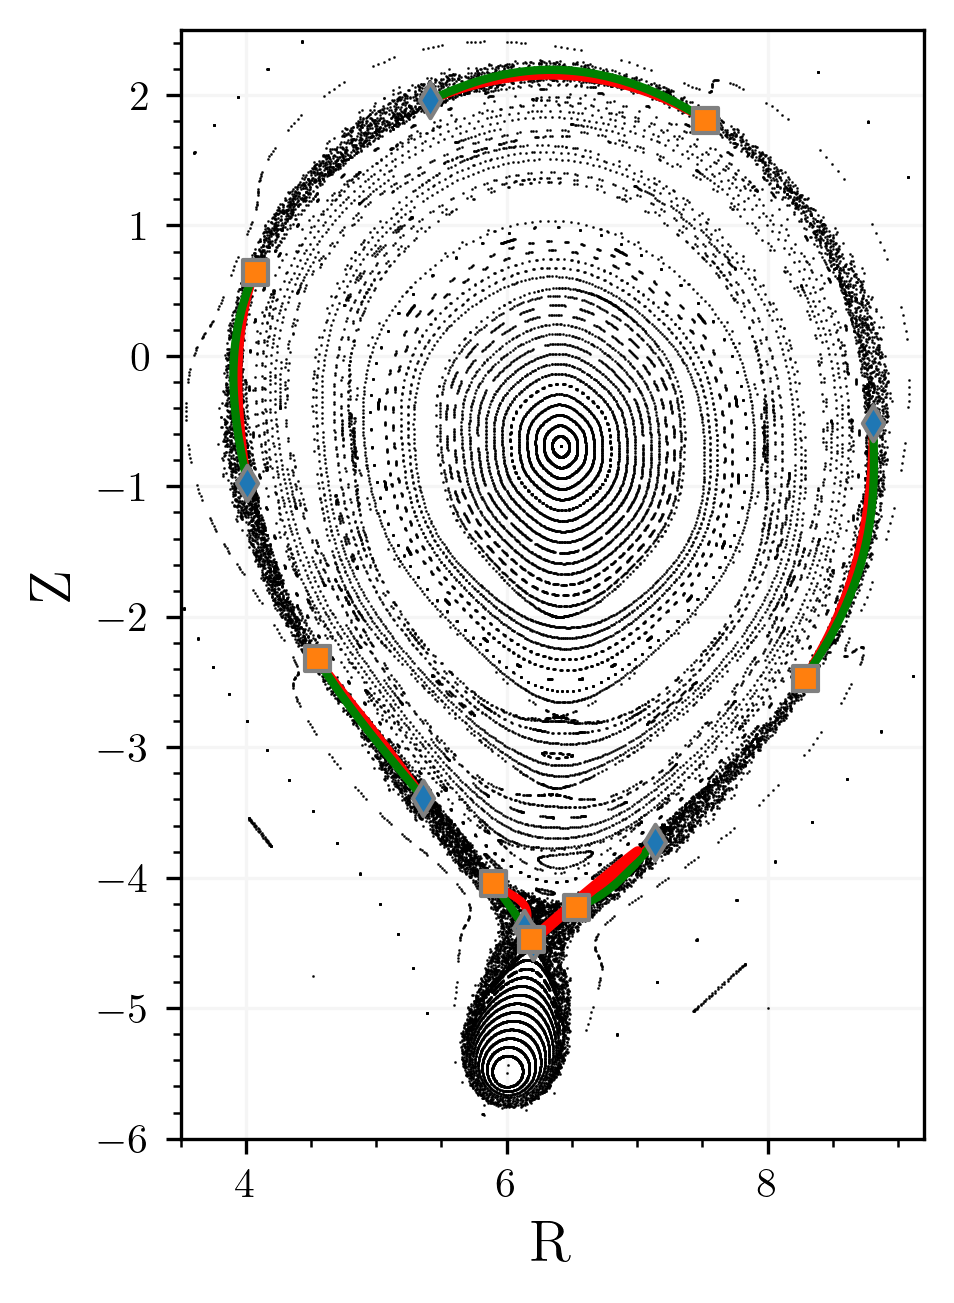
\includegraphics[width=\textwidth]{images/turnstile/coutour_fwd.png}
            \caption{}
            \label{fig:flux-poincare-conv-a}
        \end{subfigure}
    \end{minipage}
    \hfill
    \begin{minipage}[c]{0.42\textwidth} % Adjust width as needed
        \centering
        \begin{subfigure}[b]{0.95\textwidth}
            \centering
            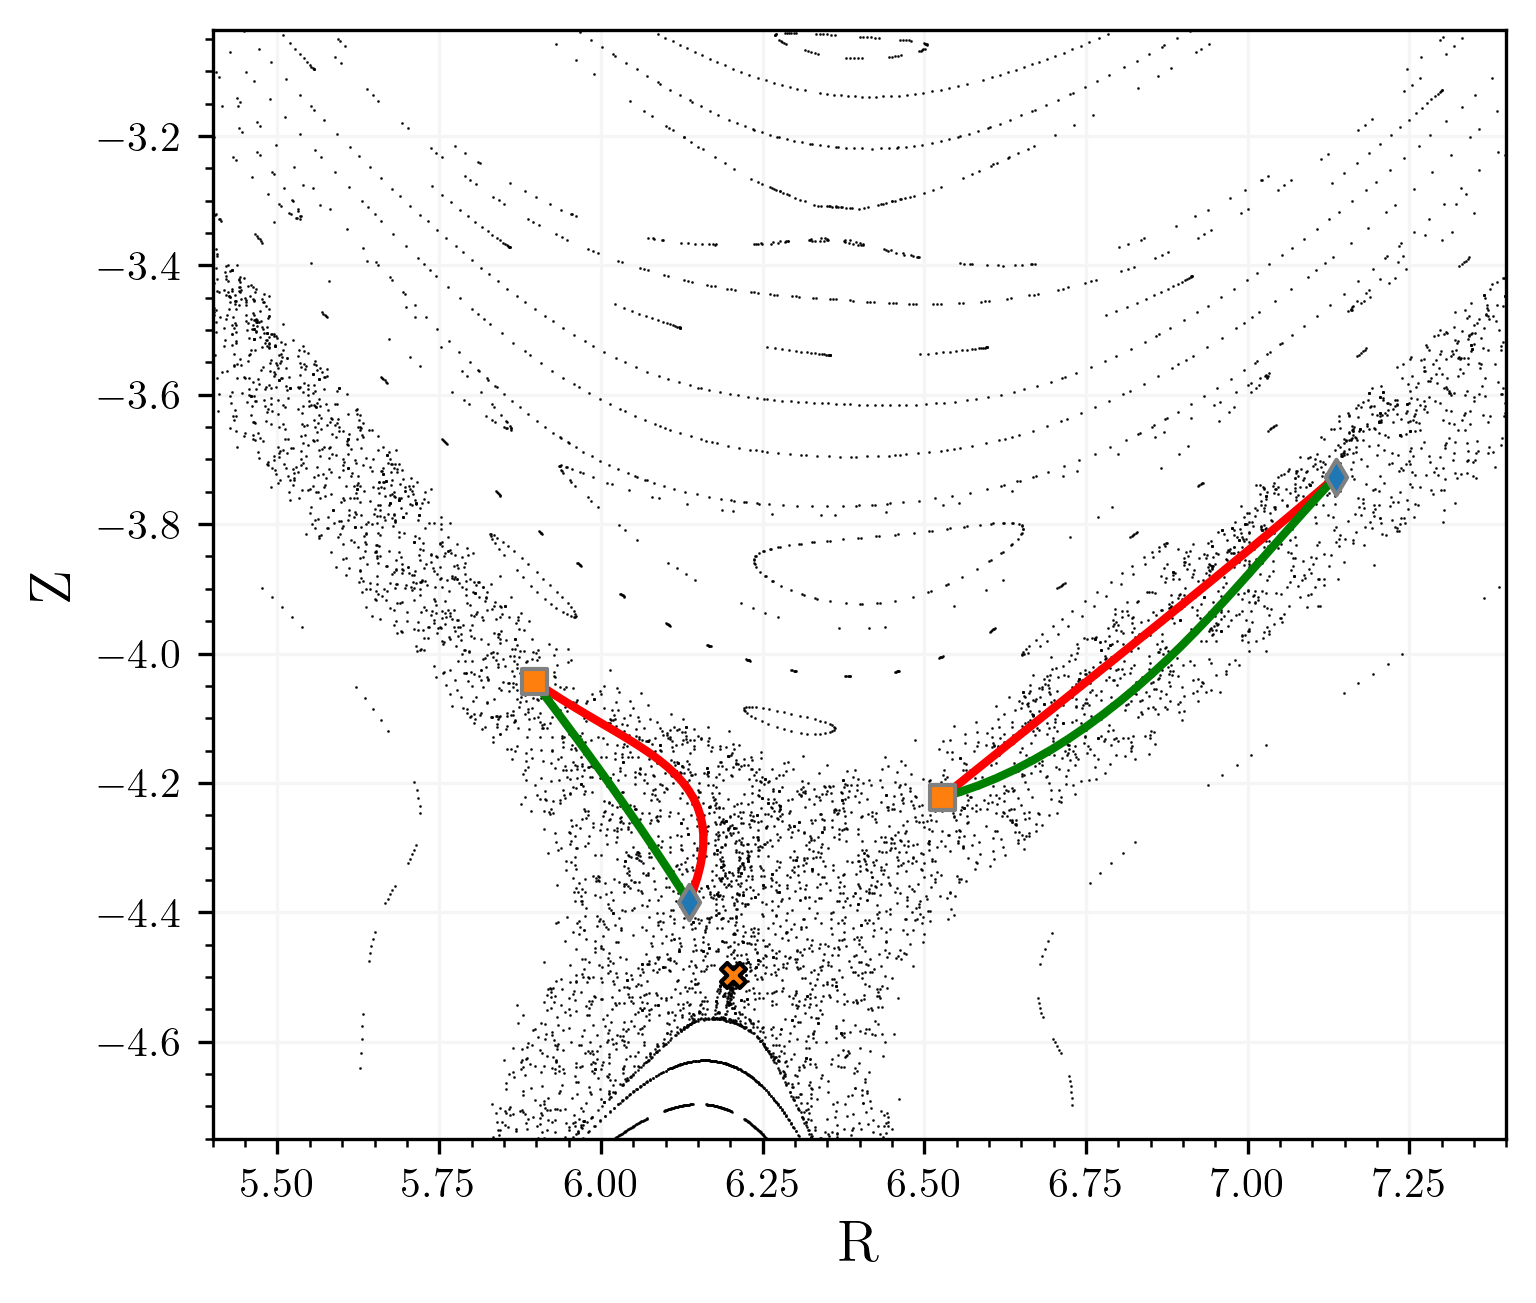
\includegraphics[width=\textwidth]{images/turnstile/coutour_c1.png}
            \caption{}
            \label{fig:flux-poincare-conv-b}
        \end{subfigure}
        \vfill
        \vspace{10px}
        \vfill
        \begin{subfigure}[b]{0.95\textwidth}
            \centering
            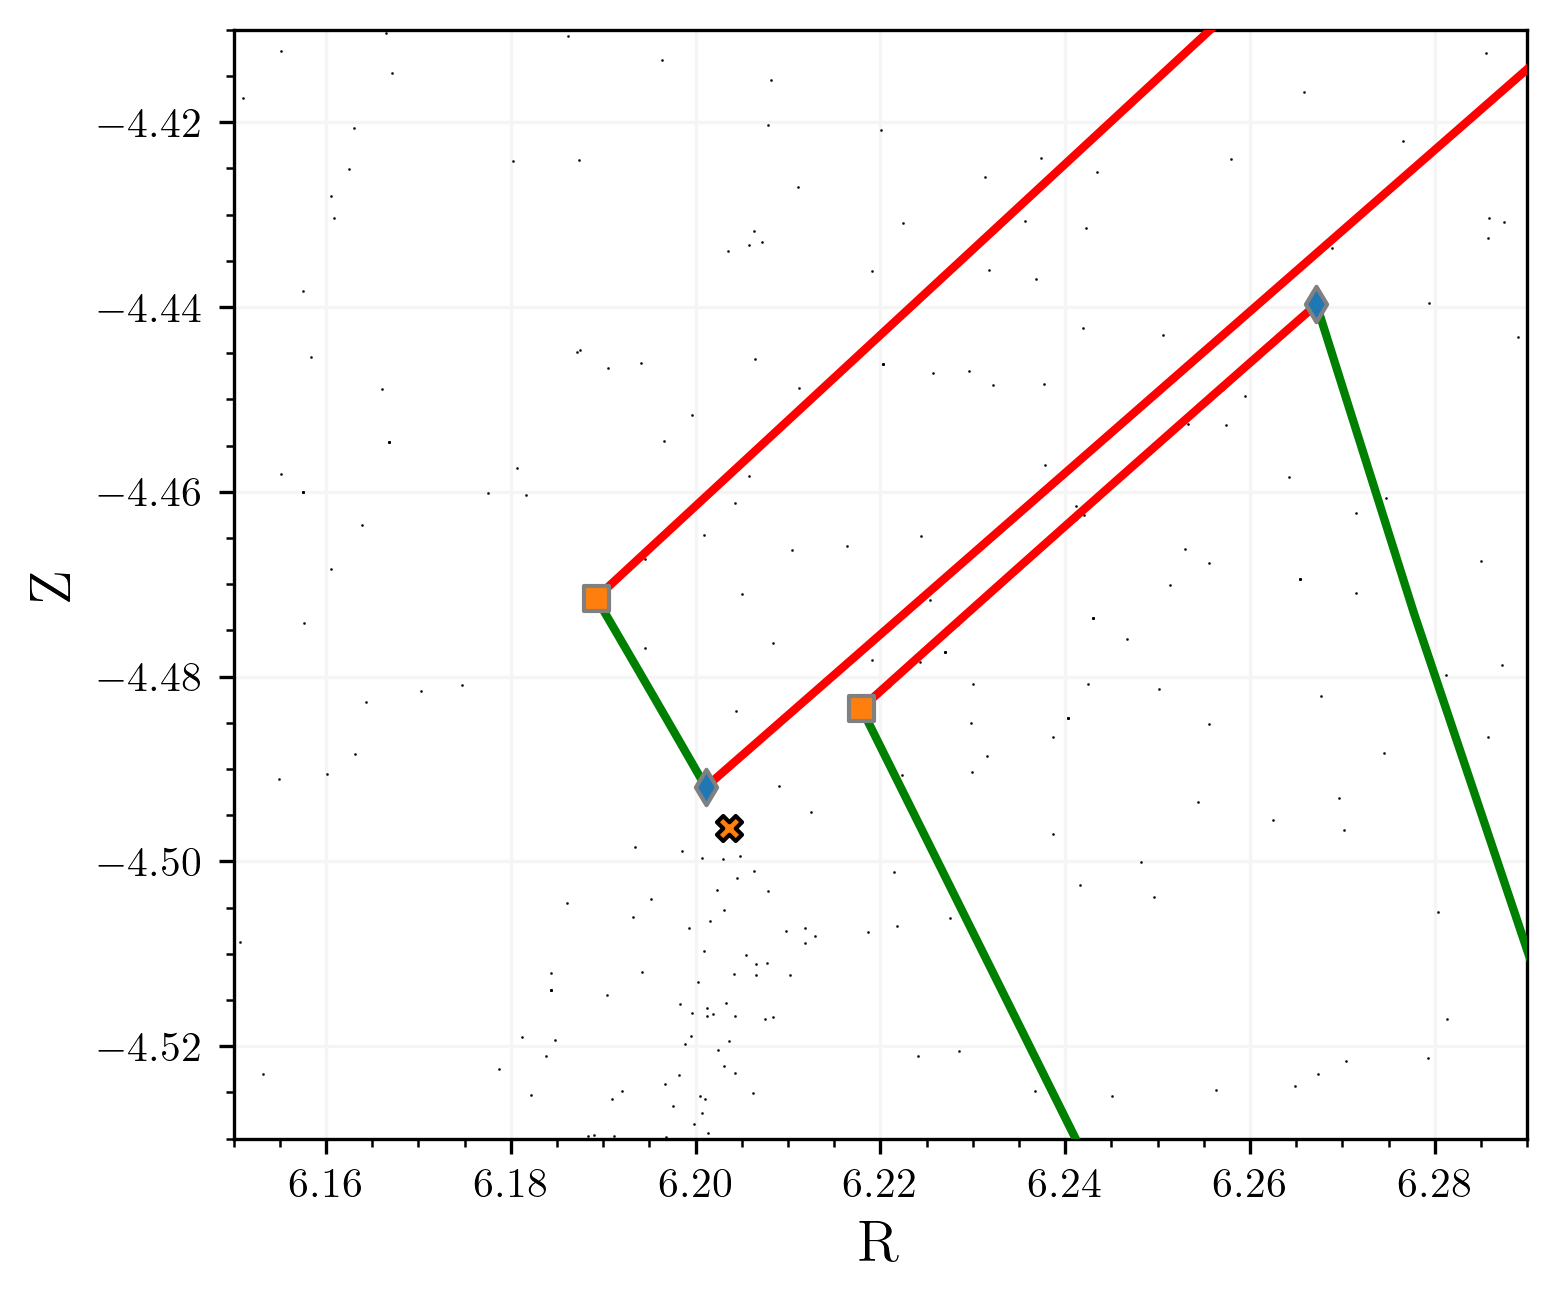
\includegraphics[width=\textwidth]{images/turnstile/coutour_c2.png}
            \caption{}
            \label{fig:flux-poincare-conv-c}
        \end{subfigure}
    \end{minipage}%
    \caption{Evolution of the turnstile lobe boundary for forward and backward iterations, note here that $\pmap$ sends points in a counterclockwise manner. The transition to the X-point can be observed in (a) where the manifolds are close to one another. In (b) and (c) the stretching of $\pmap^k(\gamma_0)$ and $\pmap^{-k}(\gamma_1)$ can be witnessed as well as the straightening/shrinking of $\pmap^{-k}(\gamma_0)$ in red and $\pmap^{k}(\gamma_1)$ in green.}
    \label{fig:flux-poincare-conv}
\end{figure}

\figref{fig:flux-poincare-conv} shows the forward and backward mappings of the contour of a lobe and thus the evolution of the joining curves. The initial lobe on low field side, exterior of the tokamak, is mapped around conter clockwise as shown in \figref{fig:flux-poincare-conv-a}. The integral on the homoclinic trajectory \eqref{eq:flux-algorithm} is shown in \figref{fig:turnstile-convergence} and for the five first iterations are done forward only and makes a transit from the HFS to the LFS and the value of the integral is jumping around. Then from that point, the last four iterations make the joining curves shrink, as shown in \figref{fig:flux-poincare-conv-b} and \figref{fig:flux-poincare-conv-c} and the integral converges. After the ninth iteration the points are again in the range where the error due to integration make the regime not linear and the point start getting further away. However as seen in \figref{fig:flux-poincare-conv-c} the can be stopped before by approximating the joining integrals where $W^s$ and $W^u$ straight. The calculation of the turnstile flux gives a numerical value of $\Phi_{lobe} = -3.879\cdot 10^{-1}$\footnote{Again without specifying the unit of the Toybox.}.

\begin{figure}[H]
    \centering
    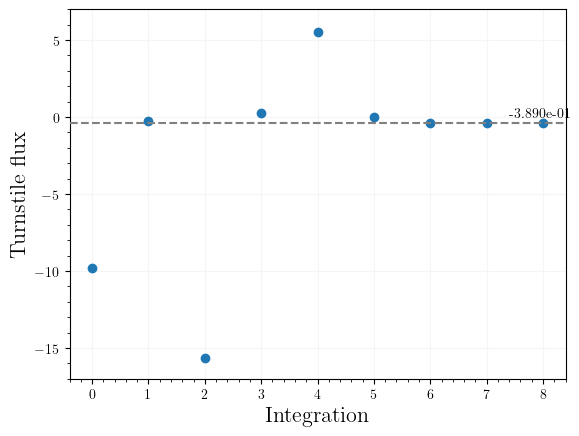
\includegraphics[width=0.7\textwidth]{images/turnstile/turnstile_area_final.png}
    \caption{Lobe flux $\Phi_{lobe}$ calculation as in \equref{eq:flux-algorithm} against the number of iteration of the Poincaré map $\pmap$. The first five iterations are done forward only. The remaining four iterations, before the integration error causes the algorithm to stop, make the joining integrals small by forward and backward iterations.}
    \label{fig:turnstile-convergence}
\end{figure}

\begin{figure}[H]
    \centering
    \begin{subfigure}[t]{0.49\textwidth}
        \centering
        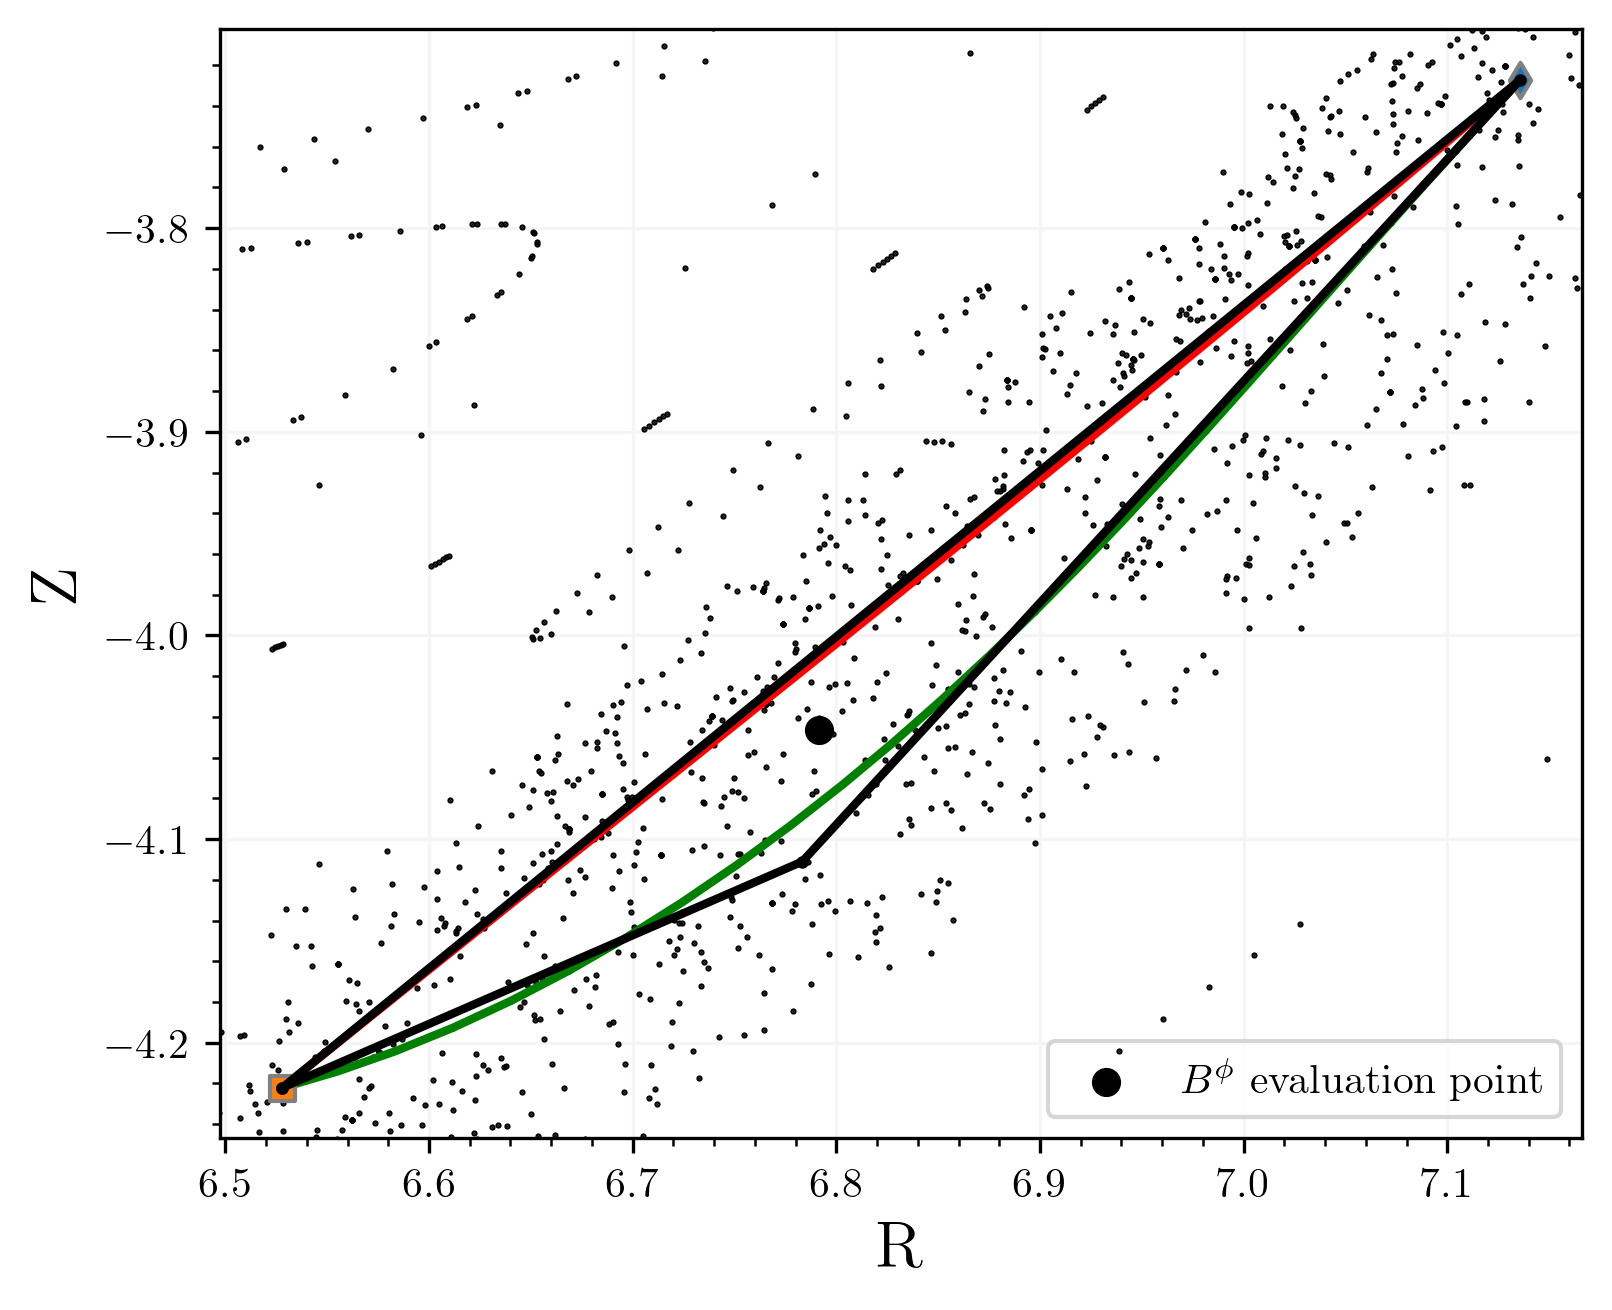
\includegraphics[width=\textwidth]{images/turnstile/verification_triangle.png}
        \caption{}
        \label{fig:verif-triangle}
    \end{subfigure}
    \hfill
    \begin{subfigure}[t]{0.49\textwidth}
        \centering
        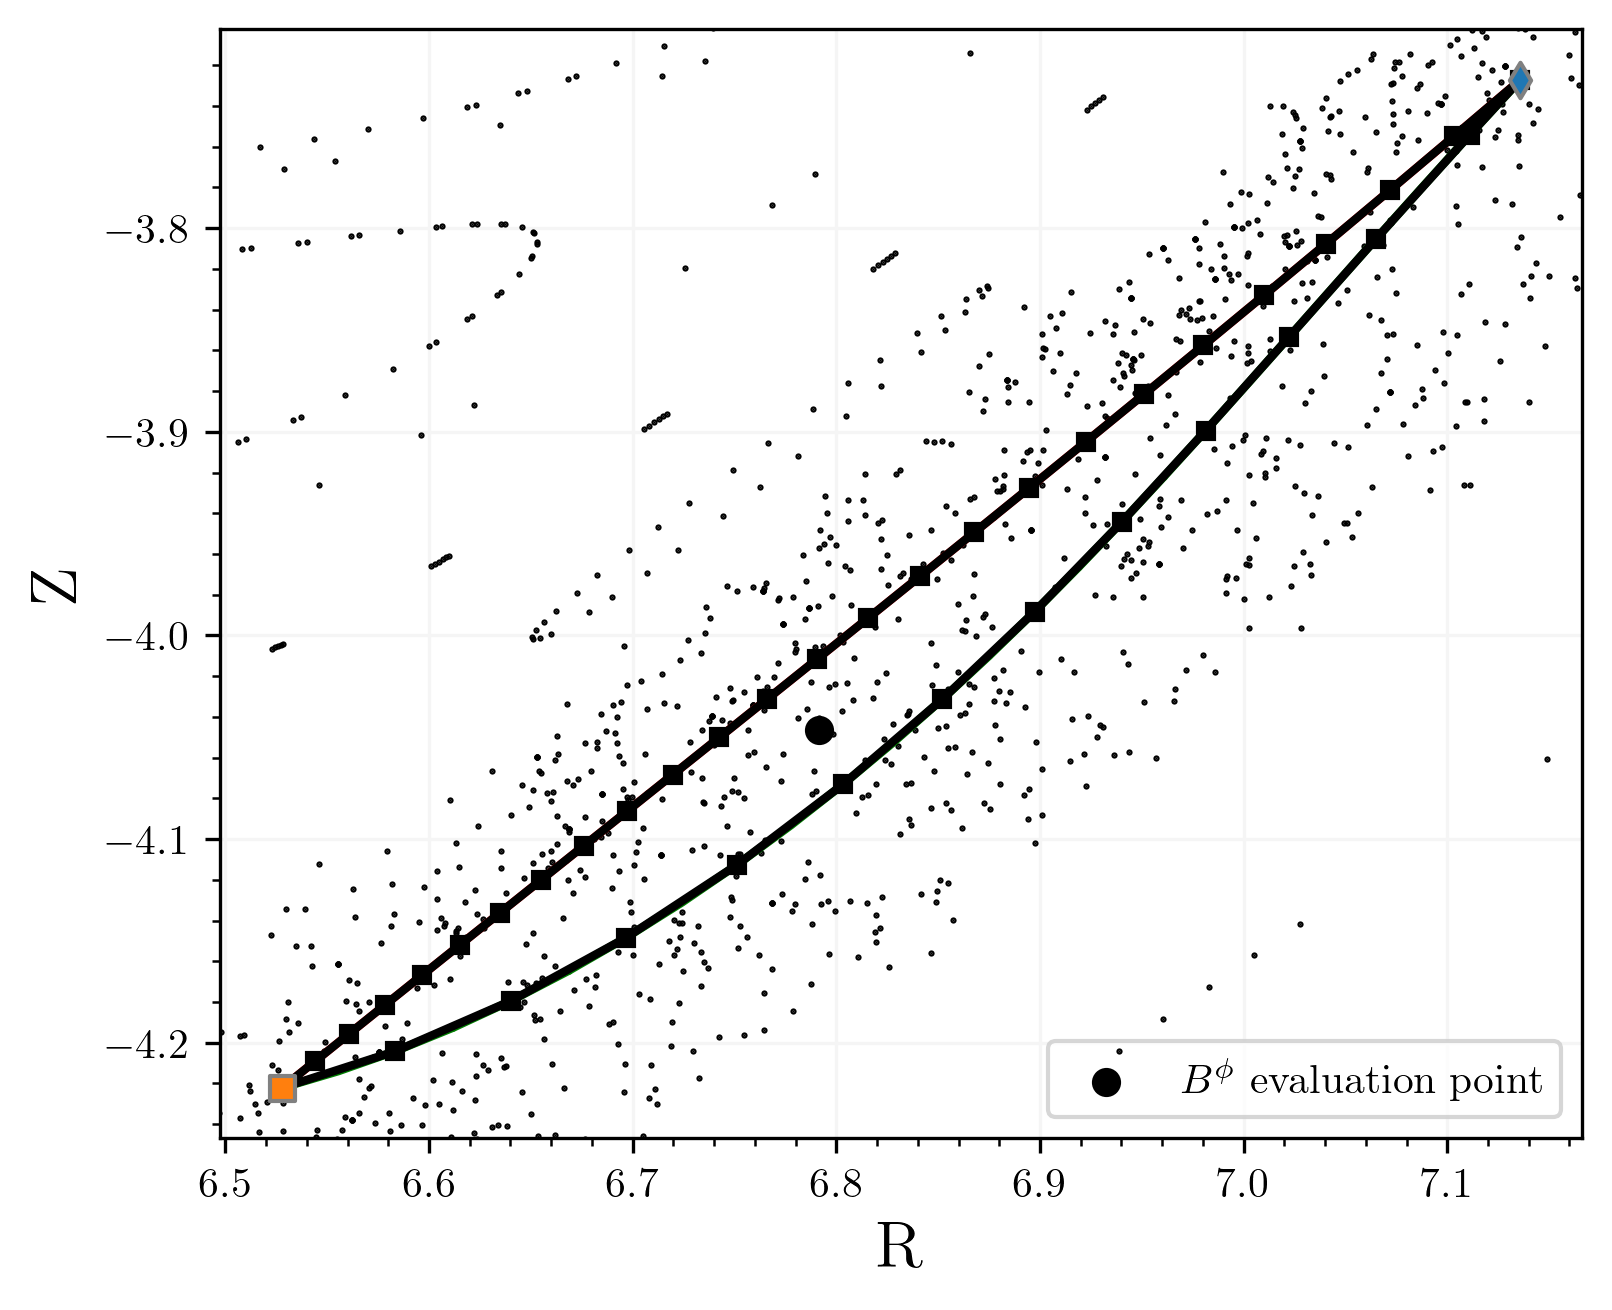
\includegraphics[width=\textwidth]{images/turnstile/verification_loop.png}
        \caption{}
        \label{fig:verif-shoelace}
    \end{subfigure}
    \caption{Surface and evaluation point for the approximation of the flux through the lobe. In (a) a simple triangle is considered and in (b) the boundary of $\Sl$ is found by tracing points in $W^s$ and $W^u$. The $B^\phi$ component of the magnetic field is evaluated at a random inner point of the lobe.}
    \label{fig:verification}
\end{figure}

To verify that the calculated value of the turnstile flux is making sense, $\Phi_{lobe}$ can be estimated using the simple approximation that~:
\begin{equation}
     \Phi_{lobe} = \int_{\Sl} \textbf{B}\cdot\textbf{dS} \approx \tilde{B}^\phi_{x_0}\,\,\vert\Sl\vert
\end{equation}
with $\tilde{B}^\phi$ evaluated at the point $x_0$ inside of the lobe and $\vert\Sl\vert$ the area of the lobe. Choosing the triangle approximation shown in \figref{fig:verif-triangle} for the surface gives an area $\vert\Sl\vert \simeq 2.9439\cdot 10^{-2}$. Evaluating $\tilde{B}^\phi$ at the point $(R, Z) = (6.791, -4.046)$, shown as the black dot, gives $\tilde{B}^\phi \simeq -14.262$ and results in an estimated value for the flux $\Phi_{lobe} \simeq -4.198\cdot 10^{-1}$, which is close to the calculated value .

This simple approximation of the area can be refined by using the so-called Shoelace formula on the boundary loop \figref{fig:verif-shoelace} computed by tracing field line : setting starting points on $W^s$ and $W^u$ in between $h$ and $m$. Using the same guess for $\tilde{B}^\phi\vert_x$ and obtaining that $\vert\Sl\vert \simeq 2.728\cdot 10^{-2}$ gives an estimated flux $\Phi_{lobe} \simeq  -3.890\cdot 10^{-1}$, even closer to the calculated flux. Finally, using the same loop, the integral of $\textbf{A}\cdot\textbf{dl}$ can also be approximated using the midpoint rule and determine $\Phi_{lobe} \simeq  -3.858\cdot 10^{-1}$. The redundancy in the value obtained here and the great agreement between them lets us believe that the turnstile flux is correctly calculated.

\subsection{Impact of the perturbation amplitude on the turnstile flux}
\newcommand{\tf}{\Phi_{lobe}}

Now that we have the calculation of the turnstile flux ready, it will be possible to determine some experimental law for its relationship in some real cases. Here however we first look at the relationship with the amplitude of the perturbation  \figref{fig:scan-6-1} gives the turnstile flux $\tf$ as a function of the amplitude for the 6/1 perturbation applied in the single null Toy-Tokamak. The evolution of $\tf$ is linear with respect to the amplitude with a slope $\approx 3.5$, it goes to zero when $\amp = 0$. For the range scanned from 0 to 0.7 there are no failure in the algorithm. For amplitude bigger we see that the process fails sometimes which is due to the homoclinic search not succeeding. The density of succeeded calculation becomes lower as more as $\amp$ is increased.

\begin{figure}[H]
    \centering
    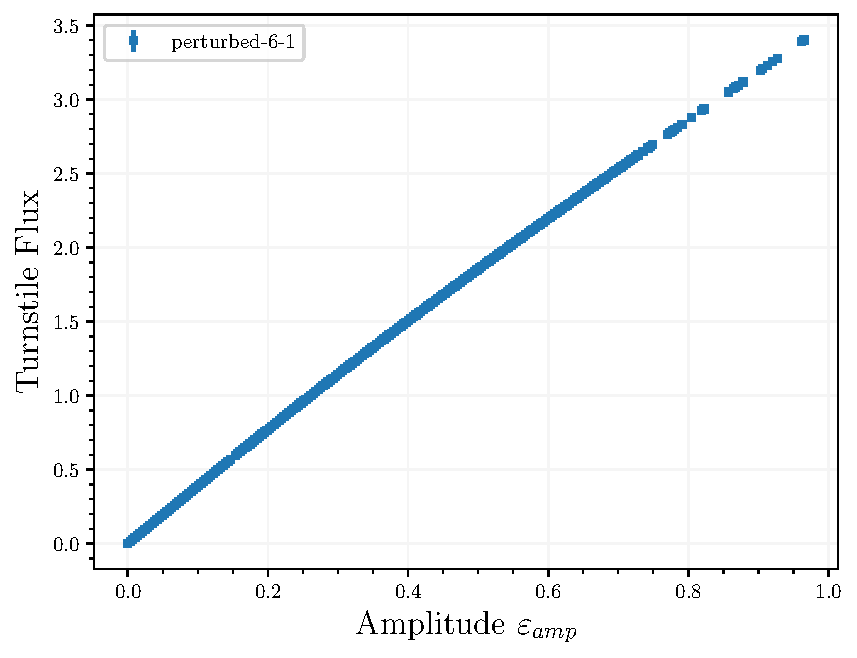
\includegraphics[width=0.7\textwidth]{images/amplitudescan/turnstile_area_6_1.pdf}
    \caption{Turnstile flux against the amplitude $\amp$ of the $6/1$ perturbation applied on the single null Toy-Tokamak equilibrium.}
    \label{fig:scan-6-1}
\end{figure}

However this was performed be trying to find automatically the two homoclinics. \figref{fig:scan-wacky} shows the poincare section for selected value of the $\amp$ between 0 and 1 ; it can be seen that the manifold structure are becoming really complicated while the algorithm is still able to find calcualte the flux for most of the time.

In the case of the 18/3 we have seen that there were 6 different homoclinic orbits to be found and actually for the 12/2 there are 4. 

\begin{figure}[H]
    \centering
    \begin{subfigure}{0.49\textwidth}
        \centering
        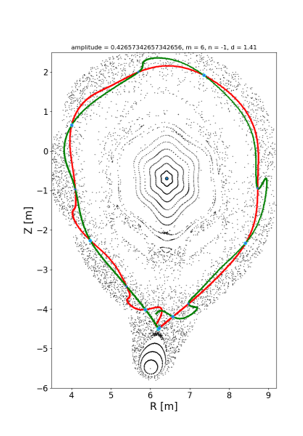
\includegraphics[width=\textwidth]{images/toytok/toytok-61-0.4.png}
        \caption{}
        \label{fig:scan-wacky-a}
    \end{subfigure}
    \begin{subfigure}{0.49\textwidth}
        \centering
        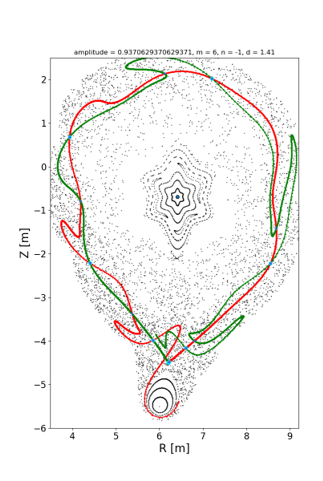
\includegraphics[width=\textwidth]{images/toytok/toytok-61-0.9.png}
        \caption{}
        \label{fig:scan-wacky-b}
    \end{subfigure}
    \caption{Poincaré section for the perturbed equilibrium with the manifold plotted at for (a) and (b).}
    \label{fig:scan-wacky}
\end{figure}

\begin{figure}[H]
    \centering
    \begin{subfigure}{0.49\textwidth}
        \centering
        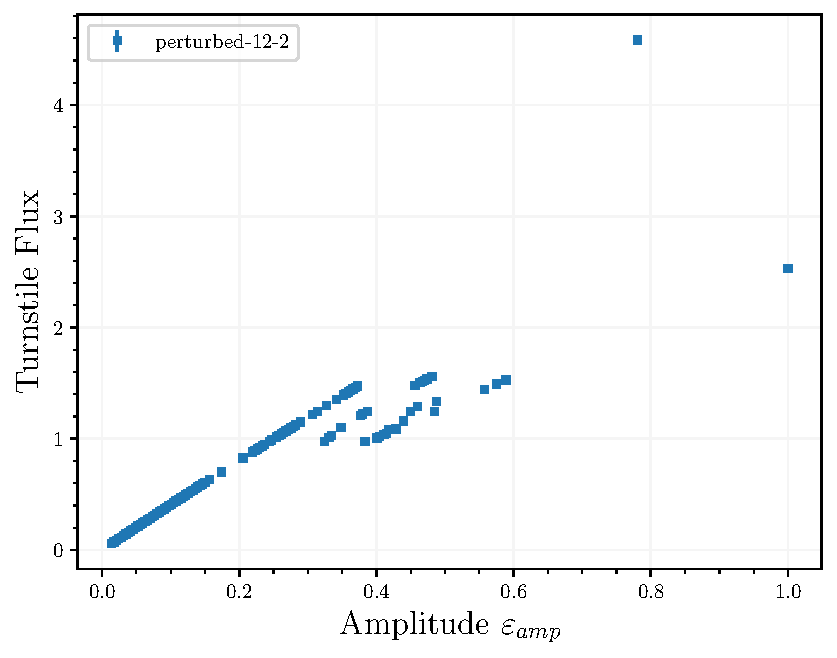
\includegraphics[width=\textwidth]{images/amplitudescan/turnstile_area_12_2.pdf}
        \caption{}
        \label{fig:scan-12-2}
    \end{subfigure}
    \begin{subfigure}{0.49\textwidth}
        \centering
        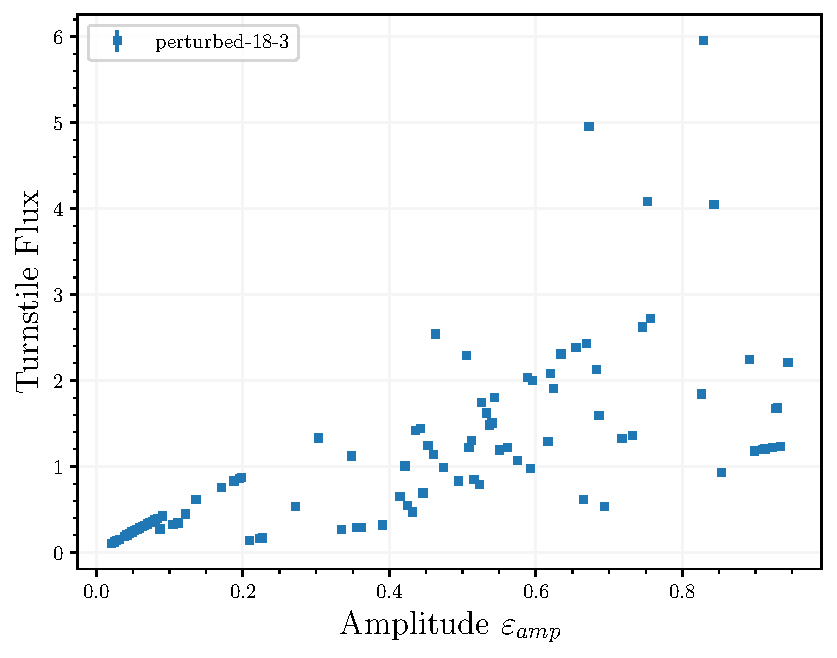
\includegraphics[width=\textwidth]{images/amplitudescan/turnstile_area_18_3.pdf}
        \caption{}
        \label{fig:scan-18-3}
    \end{subfigure}
    \caption{Turnstile flux against amplitude when applying a (a) $12/2$ and (b) $18/3$ perturbation to the single null Toy-Tokamak.}
    \label{fig:amp-scan}
\end{figure}


\subsection{Turnstiles of a $m/n$ island chain}

The turnstile calculation developed in the last sections was discussed in the case of the broken separatrix of a single null Tokamak equilibrium. However the method is not restricted to Tokamaks, or $m=1$ islands, but can be used for any islands/island chain with $\iotaslash = n/m$. The adaptation just requires to use the same amount of iteration as for finding the fixed point, effectively mapping back to the same position in the Poincaré section. In fact, as discussed in [sec], one has gcd(m,n) different islands.

\begin{figure}[h!]
    \centering
    \begin{subfigure}[c]{0.49\textwidth}
        \centering
        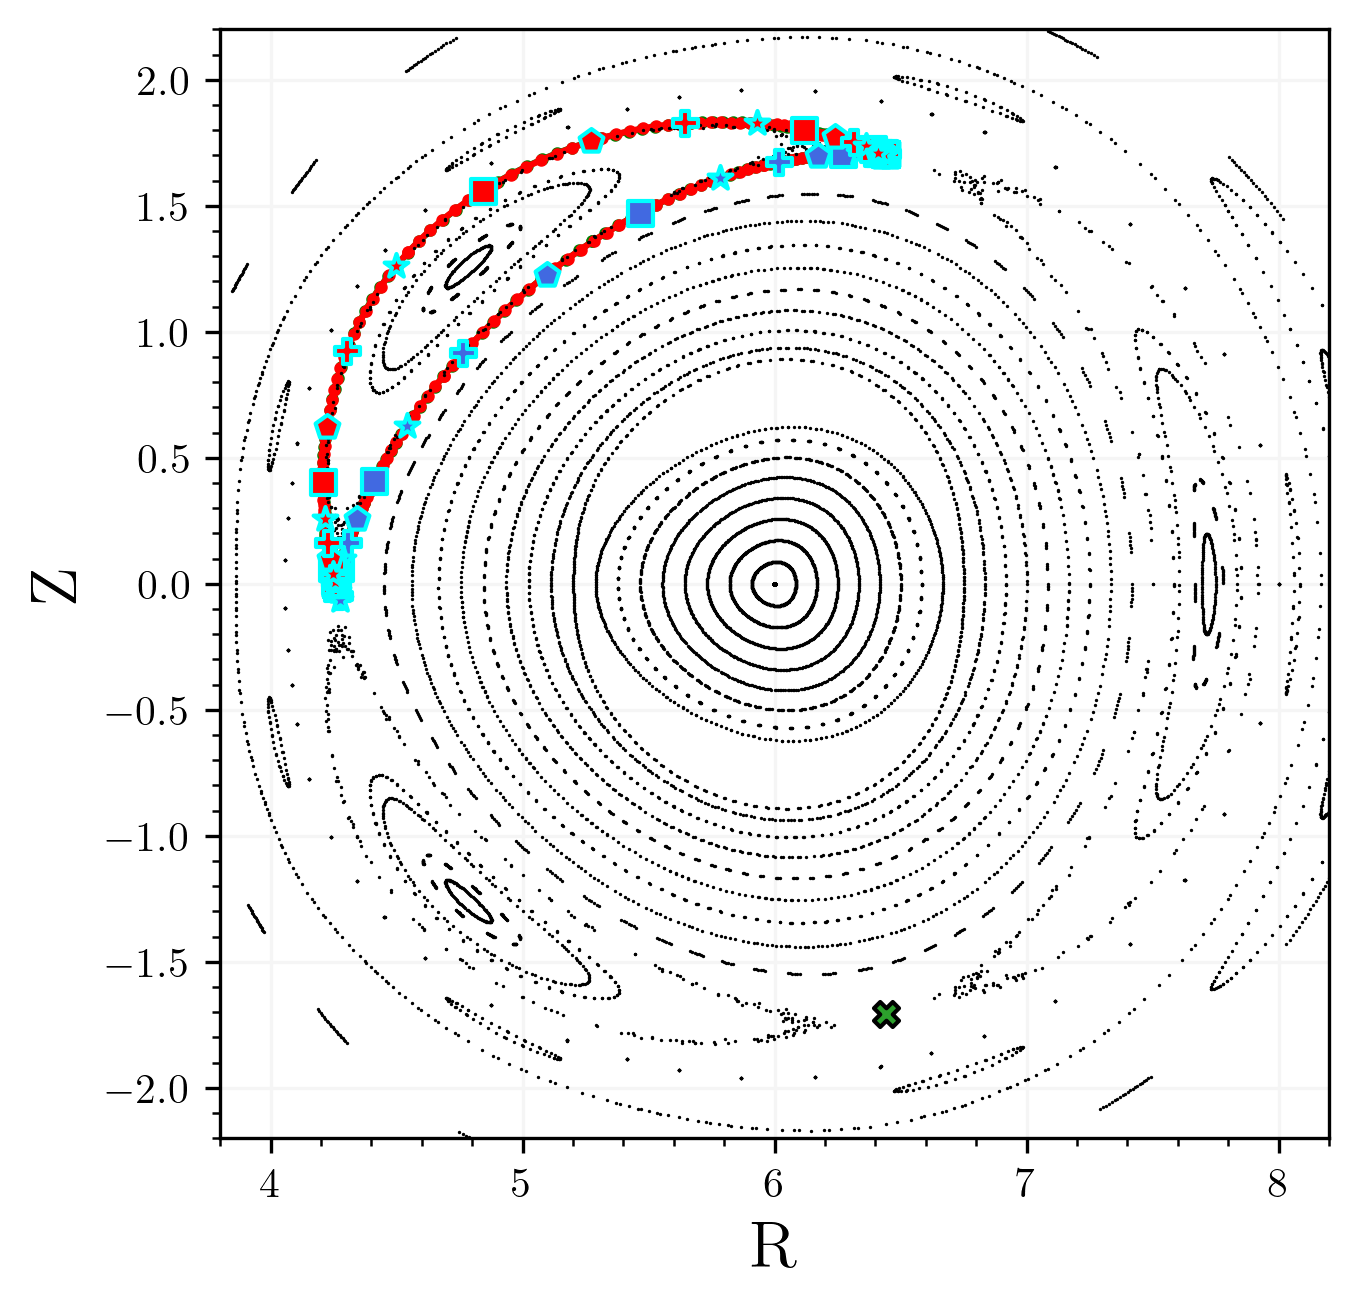
\includegraphics[width=\textwidth]{images/high-aspect-ratio/heteroclinics_outer_3.png}
        \caption{}
    \end{subfigure}
    \hfill
    \begin{subfigure}[c]{0.49\textwidth}
        \centering
        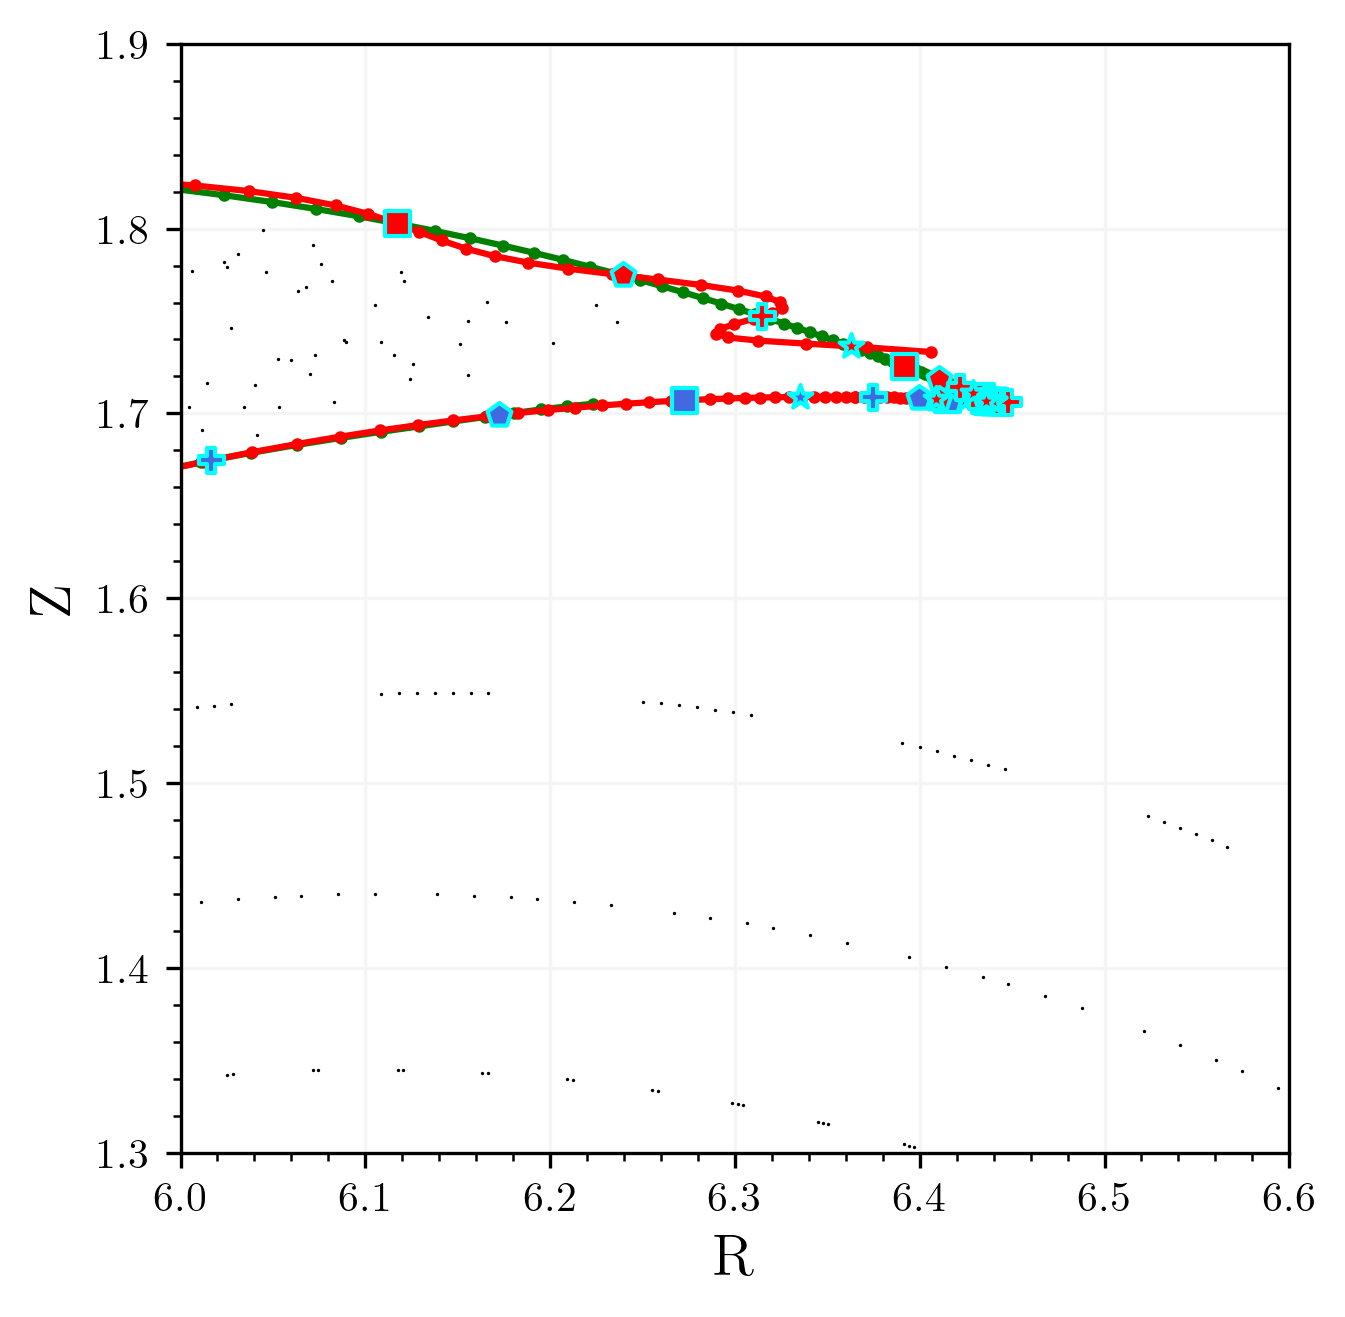
\includegraphics[width=\textwidth]{images/high-aspect-ratio/closeup.png}
        \caption{}
    \end{subfigure}
    \caption{Inner and outer stable and unstable manifolds for the high aspect ratio Tokamak equilibrium with a $m/n = 3/2$ perturbation: (a) general view, (b) zoomed in near a saddle point. The heteroclinics for inner and outer manifolds are shown.}
    \label{fig:inner-outer}
\end{figure}

In \figref{fig:inner-outer} it means for example in the case of the high aspect ratio perturbed with a $n/m = 2/3$ perturbation that

the sum of all the flux lobes gives effectively 0 further showing thet the alculation is correct.